%%%%%%%%%%%%%%%%%%%%%%%%%%%%%%%%%%%%%%%%%
% Masters/Doctoral Thesis 
% LaTeX Template
% Version 2.4 (22/11/16)
%
% This template has been downloaded from:
% http://www.LaTeXTemplates.com
%
% Version 2.x major modifications by:
% Vel (vel@latextemplates.com)
%
% This template is based on a template by:
% Steve Gunn (http://users.ecs.soton.ac.uk/srg/softwaretools/document/templates/)
% Sunil Patel (http://www.sunilpatel.co.uk/thesis-template/)
%
% Template license:
% CC BY-NC-SA 3.0 (http://creativecommons.org/licenses/by-nc-sa/3.0/)
%
%%%%%%%%%%%%%%%%%%%%%%%%%%%%%%%%%%%%%%%%%

%----------------------------------------------------------------------------------------
%	PACKAGES AND OTHER DOCUMENT CONFIGURATIONS
%----------------------------------------------------------------------------------------

\documentclass[
11pt, % The default document font size, options: 10pt, 11pt, 12pt
%oneside, % Two side (alternating margins) for binding by default, uncomment to switch to one side
english, % ngerman for German
singlespacing, % Single line spacing, alternatives: onehalfspacing or doublespacing
%draft, % Uncomment to enable draft mode (no pictures, no links, overfull hboxes indicated)
%nolistspacing, % If the document is onehalfspacing or doublespacing, uncomment this to set spacing in lists to single
%liststotoc, % Uncomment to add the list of figures/tables/etc to the table of contents
%toctotoc, % Uncomment to add the main table of contents to the table of contents
%parskip, % Uncomment to add space between paragraphs
%nohyperref, % Uncomment to not load the hyperref package
%headsepline, % Uncomment to get a line under the header
%chapterinoneline, % Uncomment to place the chapter title next to the number on one line
%consistentlayout, % Uncomment to change the layout of the declaration, abstract and acknowledgements pages to match the default layout
]{MastersDoctoralThesis} % The class file specifying the document structure

%\usepackage[utf8]{inputenc} % Required for inputting international characters
\usepackage[T1]{fontenc} % Output font encoding for international characters

\usepackage{palatino} % Use the Palatino font by default

\usepackage[backend=bibtex,style=authoryear,natbib=true]{biblatex} % Use the bibtex backend with the authoryear citation style (which resembles APA)

\addbibresource{example.bib} % The filename of the bibliography

\usepackage[autostyle=true]{csquotes} % Required to generate language-dependent quotes in the bibliography

%----------------------------------------------------------------------------------------
%	MARGIN SETTINGS
%----------------------------------------------------------------------------------------

\geometry{
	paper=a4paper, % Change to letterpaper for US letter
	inner=2.5cm, % Inner margin
	outer=3.8cm, % Outer margin
	bindingoffset=.5cm, % Binding offset
	top=1.5cm, % Top margin
	bottom=1.5cm, % Bottom margin
	%showframe, % Uncomment to show how the type block is set on the page
}

%----------------------------------------------------------------------------------------
%	THESIS INFORMATION
%----------------------------------------------------------------------------------------

\thesistitle{Formaci\'on de galaxias barradas en simulaciones num\'ericas del Grupo Local} % Your thesis title, this is used in the title and abstract, print it elsewhere with \ttitle
\supervisor{Dr. Mario G. \textsc{Abadi}} % Your supervisor's name, this is used in the title page, print it elsewhere with \supname
\examiner{} % Your examiner's name, this is not currently used anywhere in the template, print it elsewhere with \examname
\degree{Licenciada en Astronom\'ia} % Your degree name, this is used in the title page and abstract, print it elsewhere with \degreename
\author{Ornela F. \textsc{Marioni}} % Your name, this is used in the title page and abstract, print it elsewhere with \authorname
\addresses{} % Your address, this is not currently used anywhere in the template, print it elsewhere with \addressname

\subject{Astronom\'ia} % Your subject area, this is not currently used anywhere in the template, print it elsewhere with \subjectname
\keywords{} % Keywords for your thesis, this is not currently used anywhere in the template, print it elsewhere with \keywordnames
\university{\href{http://www.unc.edu.ar/}{Universidad Nacional de C\'ordoba}} % Your university's name and URL, this is used in the title page and abstract, print it elsewhere with \univname
\department{\href{http://department.university.com}{Department or School Name}} % Your department's name and URL, this is used in the title page and abstract, print it elsewhere with \deptname
\group{\href{http://researchgroup.university.com}{Research Group Name}} % Your research group's name and URL, this is used in the title page, print it elsewhere with \groupname
\faculty{\href{http://www.famaf.unc.edu.ar/}{Facultad de Matem\'atica, Astronom\'ia, F\'isica y Computaci\'on}} % Your faculty's name and URL, this is used in the title page and abstract, print it elsewhere with \facname

\AtBeginDocument{
\hypersetup{pdftitle=\ttitle} % Set the PDF's title to your title
\hypersetup{pdfauthor=\authorname} % Set the PDF's author to your name
\hypersetup{pdfkeywords=\keywordnames} % Set the PDF's keywords to your keywords
}

\begin{document}

\frontmatter % Use roman page numbering style (i, ii, iii, iv...) for the pre-content pages

\pagestyle{plain} % Default to the plain heading style until the thesis style is called for the body content

%----------------------------------------------------------------------------------------
%	TITLE PAGE
%----------------------------------------------------------------------------------------

\begin{titlepage}
\begin{center}

\vspace*{.06\textheight}
{\scshape\LARGE \univname\par}\vspace{1.5cm} % University name
\textsc{\Large Trabajo Final de Licenciatura}\\[0.5cm] % Thesis type

\HRule \\[0.4cm] % Horizontal line
{\huge \bfseries \ttitle\par}\vspace{0.4cm} % Thesis title
\HRule \\[1.5cm] % Horizontal line
 
\begin{minipage}[t]{0.4\textwidth}
\begin{flushleft} \large
\emph{Autor:}\\
\authorname % Author name - remove the \href bracket to remove the link

\end{flushleft}
\end{minipage}
\begin{minipage}[t]{0.4\textwidth}
\begin{flushright} \large
\emph{Director:} \\
%\href{http://www.jamessmith.com}{\supname} % Supervisor name - remove the \href bracket to remove the link  
\supname

\end{flushright}
\end{minipage}\\[3cm]
 
\vfill

%\large \textit{Trabajo final de Licenciatura\\ para obtener el t\'itulo de \degreename}\\[0.3cm] % University requirement text
%\textit{in the}\\[0.4cm]
%\groupname\\\deptname\\[2cm] % Research group name and department name
 
\vfill

{\large \today}\\[4cm] % Date
%\includegraphics{Logo} % University/department logo - uncomment to place it
 
\vfill
\end{center}
\end{titlepage}

%----------------------------------------------------------------------------------------
%	DECLARATION PAGE
%----------------------------------------------------------------------------------------

%\begin{declaration}
%\addchaptertocentry{\authorshipname} % Add the declaration to the table of contents
%\noindent I, \authorname, declare that this thesis titled, \enquote{\ttitle} and the work presented in it are my own. I confirm that:

%\begin{itemize} 
%\item This work was done wholly or mainly while in candidature for a research degree at this University.
%\item Where any part of this thesis has previously been submitted for a degree or any other qualification at this University or any other institution, this has been clearly stated.
%\item Where I have consulted the published work of others, this is always clearly attributed.
%0\item Where I have quoted from the work of others, the source is always given. With the exception of such quotations, this thesis is entirely my own work.
%\item I have acknowledged all main sources of help.
%\item Where the thesis is based on work done by myself jointly with others, I have made clear exactly what was done by others and what I have contributed myself.\\
%\end{itemize}
 
%\noindent Signed:\\
%\rule[0.5em]{25em}{0.5pt} % This prints a line for the signature
 
%\noindent Date:\\
%\rule[0.5em]{25em}{0.5pt} % This prints a line to write the date
%\end{declaration}

%\cleardoublepage

%----------------------------------------------------------------------------------------
%	QUOTATION PAGE
%----------------------------------------------------------------------------------------

\vspace*{0.2\textheight}

\noindent\enquote{\itshape Thanks to my solid academic training, today I can write hundreds of words on virtually any topic without possessing a shred of information, which is how I got a good job in journalism.}\bigbreak

\hfill Dave Barry

%----------------------------------------------------------------------------------------
%	ABSTRACT PAGE
%----------------------------------------------------------------------------------------

\begin{abstract}
\addchaptertocentry{\abstractname} % Add the abstract to the table of contents
The Thesis Abstract is written here (and usually kept to just this page). The page is kept centered vertically so can expand into the blank space above the title too\ldots
\end{abstract}

%----------------------------------------------------------------------------------------
%	ACKNOWLEDGEMENTS
%----------------------------------------------------------------------------------------

\begin{acknowledgements}
\addchaptertocentry{\acknowledgementname} % Add the acknowledgements to the table of contents
The acknowledgments and the people to thank go here, don't forget to include your project advisor\ldots
\end{acknowledgements}

%----------------------------------------------------------------------------------------
%	LIST OF CONTENTS/FIGURES/TABLES PAGES
%----------------------------------------------------------------------------------------

\tableofcontents % Prints the main table of contents

\listoffigures % Prints the list of figures

\listoftables % Prints the list of tables

%----------------------------------------------------------------------------------------
%	ABBREVIATIONS
%----------------------------------------------------------------------------------------

\begin{abbreviations}{ll} % Include a list of abbreviations (a table of two columns)

\textbf{LAH} & \textbf{L}ist \textbf{A}bbreviations \textbf{H}ere\\
\textbf{WSF} & \textbf{W}hat (it) \textbf{S}tands \textbf{F}or\\

\end{abbreviations}

%----------------------------------------------------------------------------------------
%	PHYSICAL CONSTANTS/OTHER DEFINITIONS
%----------------------------------------------------------------------------------------

\begin{constants}{lr@{${}={}$}l} % The list of physical constants is a three column table

% The \SI{}{} command is provided by the siunitx package, see its documentation for instructions on how to use it

Speed of Light & $c_{0}$ & \SI{2.99792458e8}{\meter\per\second} (exact)\\
%Constant Name & $Symbol$ & $Constant Value$ with units\\

\end{constants}

%----------------------------------------------------------------------------------------
%	SYMBOLS
%----------------------------------------------------------------------------------------

\begin{symbols}{lll} % Include a list of Symbols (a three column table)

$a$ & distance & \si{\meter} \\
$P$ & power & \si{\watt} (\si{\joule\per\second}) \\
%Symbol & Name & Unit \\

\addlinespace % Gap to separate the Roman symbols from the Greek

$\omega$ & angular frequency & \si{\radian} \\

\end{symbols}

%----------------------------------------------------------------------------------------
%	DEDICATION
%----------------------------------------------------------------------------------------

\dedicatory{For/Dedicated to/To my\ldots} 

%----------------------------------------------------------------------------------------
%	THESIS CONTENT - CHAPTERS
%----------------------------------------------------------------------------------------

\mainmatter % Begin numeric (1,2,3...) page numbering

\pagestyle{thesis} % Return the page headers back to the "thesis" style

% Include the chapters of the thesis as separate files from the Chapters folder
% Uncomment the lines as you write the chapters

% Chapter 1

\chapter{GAS/DM} % Main chapter title

\label{Chapter1} % For referencing the chapter elsewhere, use \ref{Chapter1} 

%----------------------------------------------------------------------------------------

% Define some commands to keep the formatting separated from the content 
\newcommand{\keyword}[1]{\textbf{#1}}
\newcommand{\tabhead}[1]{\textbf{#1}}
\newcommand{\code}[1]{\texttt{#1}}
\newcommand{\file}[1]{\texttt{\bfseries#1}}
\newcommand{\option}[1]{\texttt{\itshape#1}}

%----------------------------------------------------------------------------------------

\section{}









\section{Figures}


\begin{figure}[h]
\centering
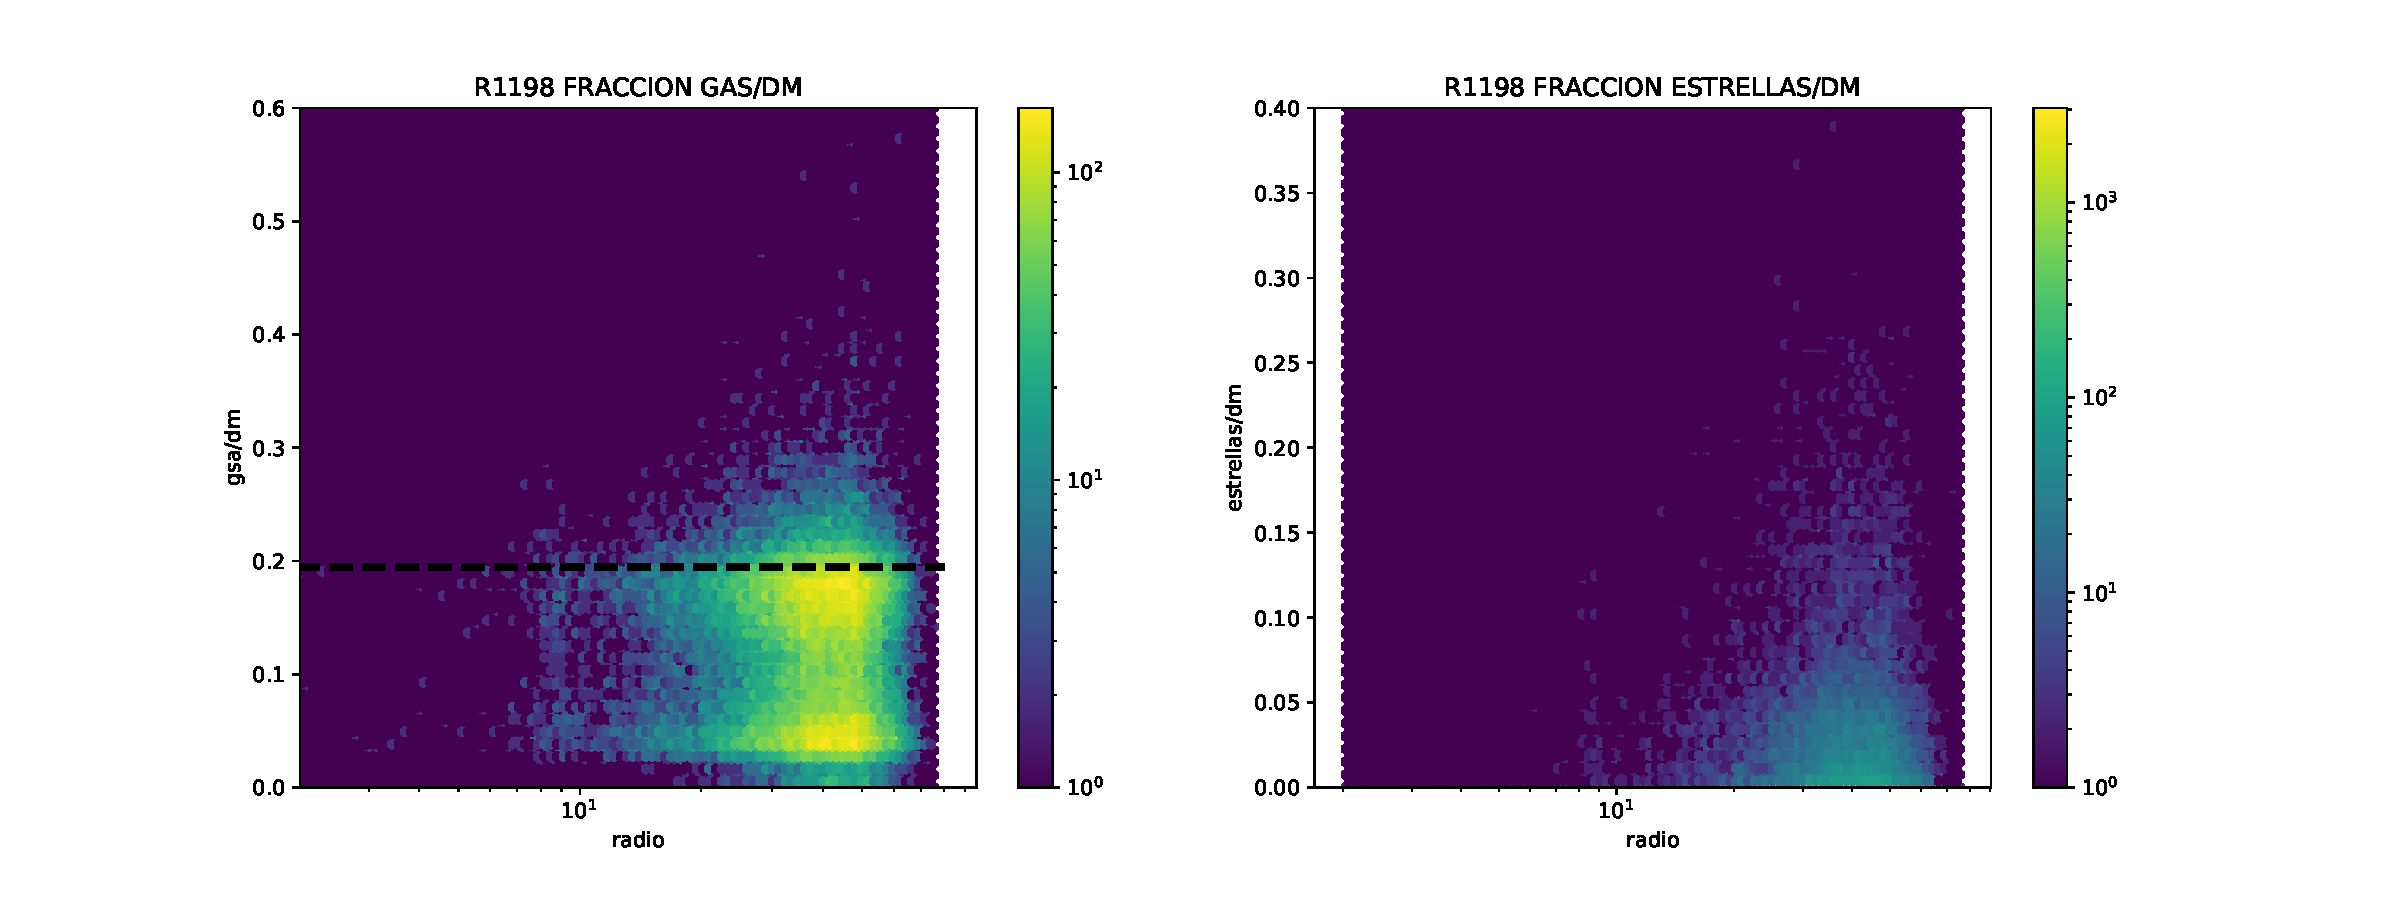
\includegraphics[width=1\textwidth]{Figures/R1198_scatterFRACCIONES.pdf}
\decoRule
\caption[R1198 BARIONES/DM perfil (scatter) ]{Fraccion de gas sobre DM en funcion del centro del void, tamaño del void $\sim$ 9.5 Mpc. A la derecha la fraccion es de Estrellas sobre DM}
\label{fig:Electron}
\end{figure}

\begin{figure}[h]
\centering
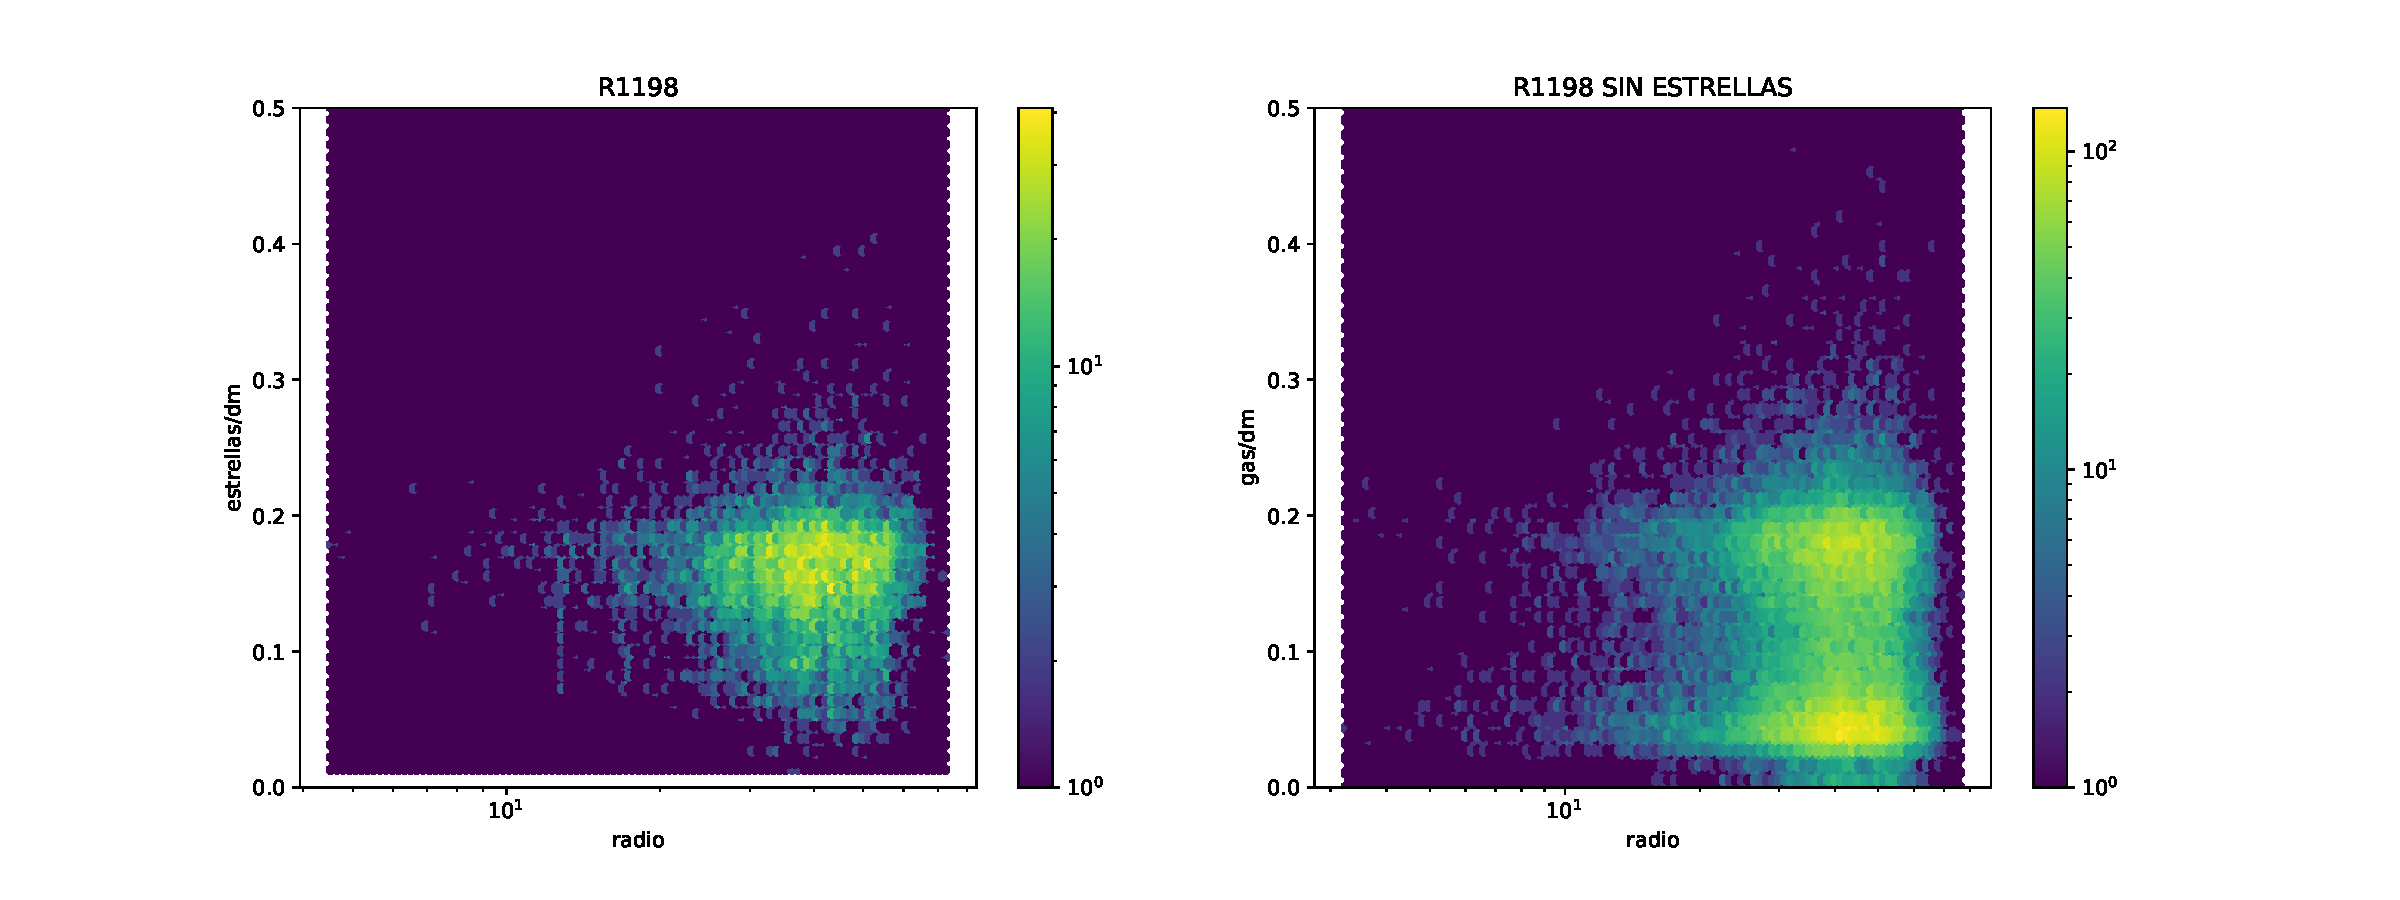
\includegraphics[width=1\textwidth]{Figures/R1198_scatterFRACCIONES_con&sinEST.pdf}
\decoRule
\caption[R1198 GAS/DM perfil (scatter) con y sin estrells]{Perfil de gas/dm para los halos. A  la izquierda estan los halos que contienen al menos una particula de estrellas. A la derehc a los que no tienen ninguna estrella}
\label{fig:Electron}
\end{figure}

\begin{figure}[h]
\centering
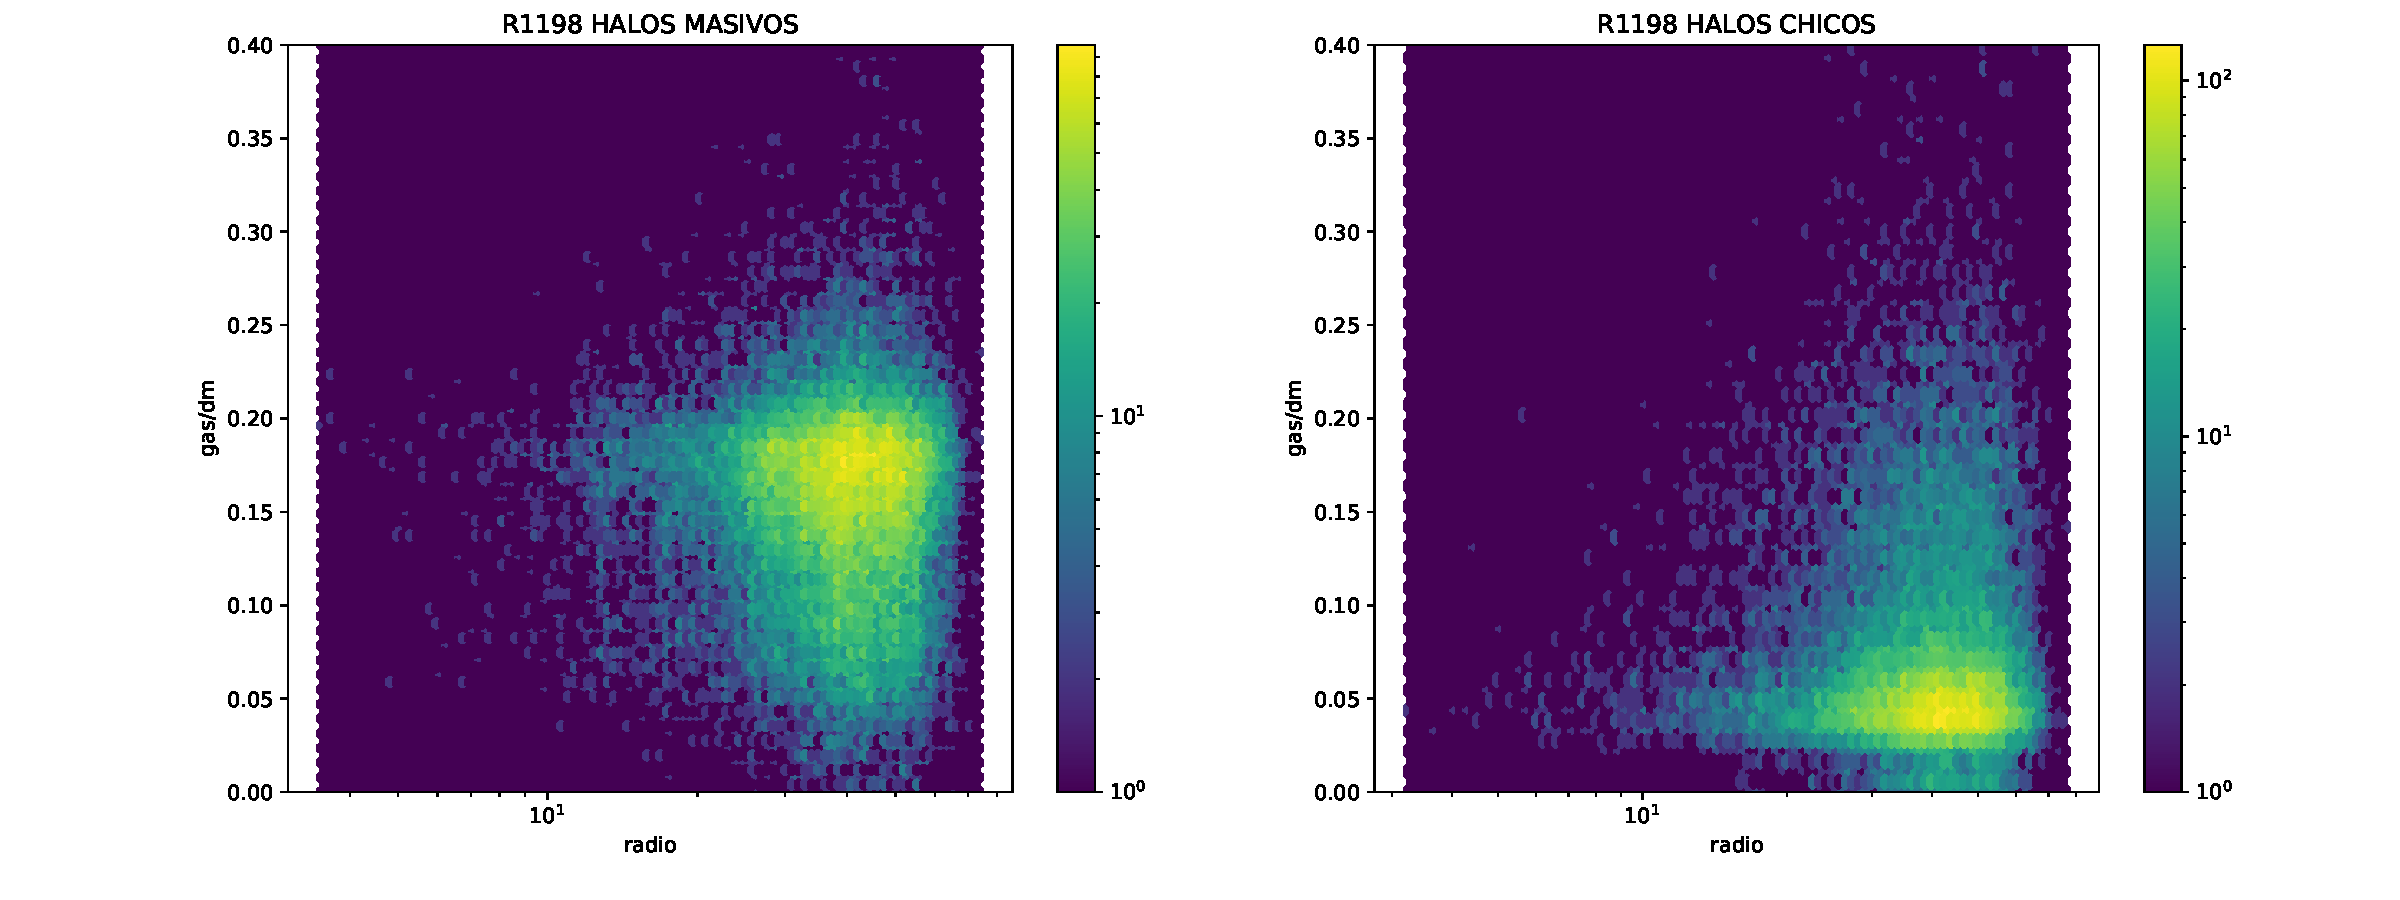
\includegraphics[width=1\textwidth]{Figures/R1198_scatterFRACCIONES_grandesYchicos.pdf}
\decoRule
\caption[R1198 GAS/DM perfil (scatter) halos grandes y chisos]{fraccion de gas sobre DM separando los halos por tamaño. Los halos GRANDES tienen mas de 50 particulas de DM, los chicos menos de 50. }
\label{fig:Electron}
\end{figure}


\begin{figure}[h]
\centering
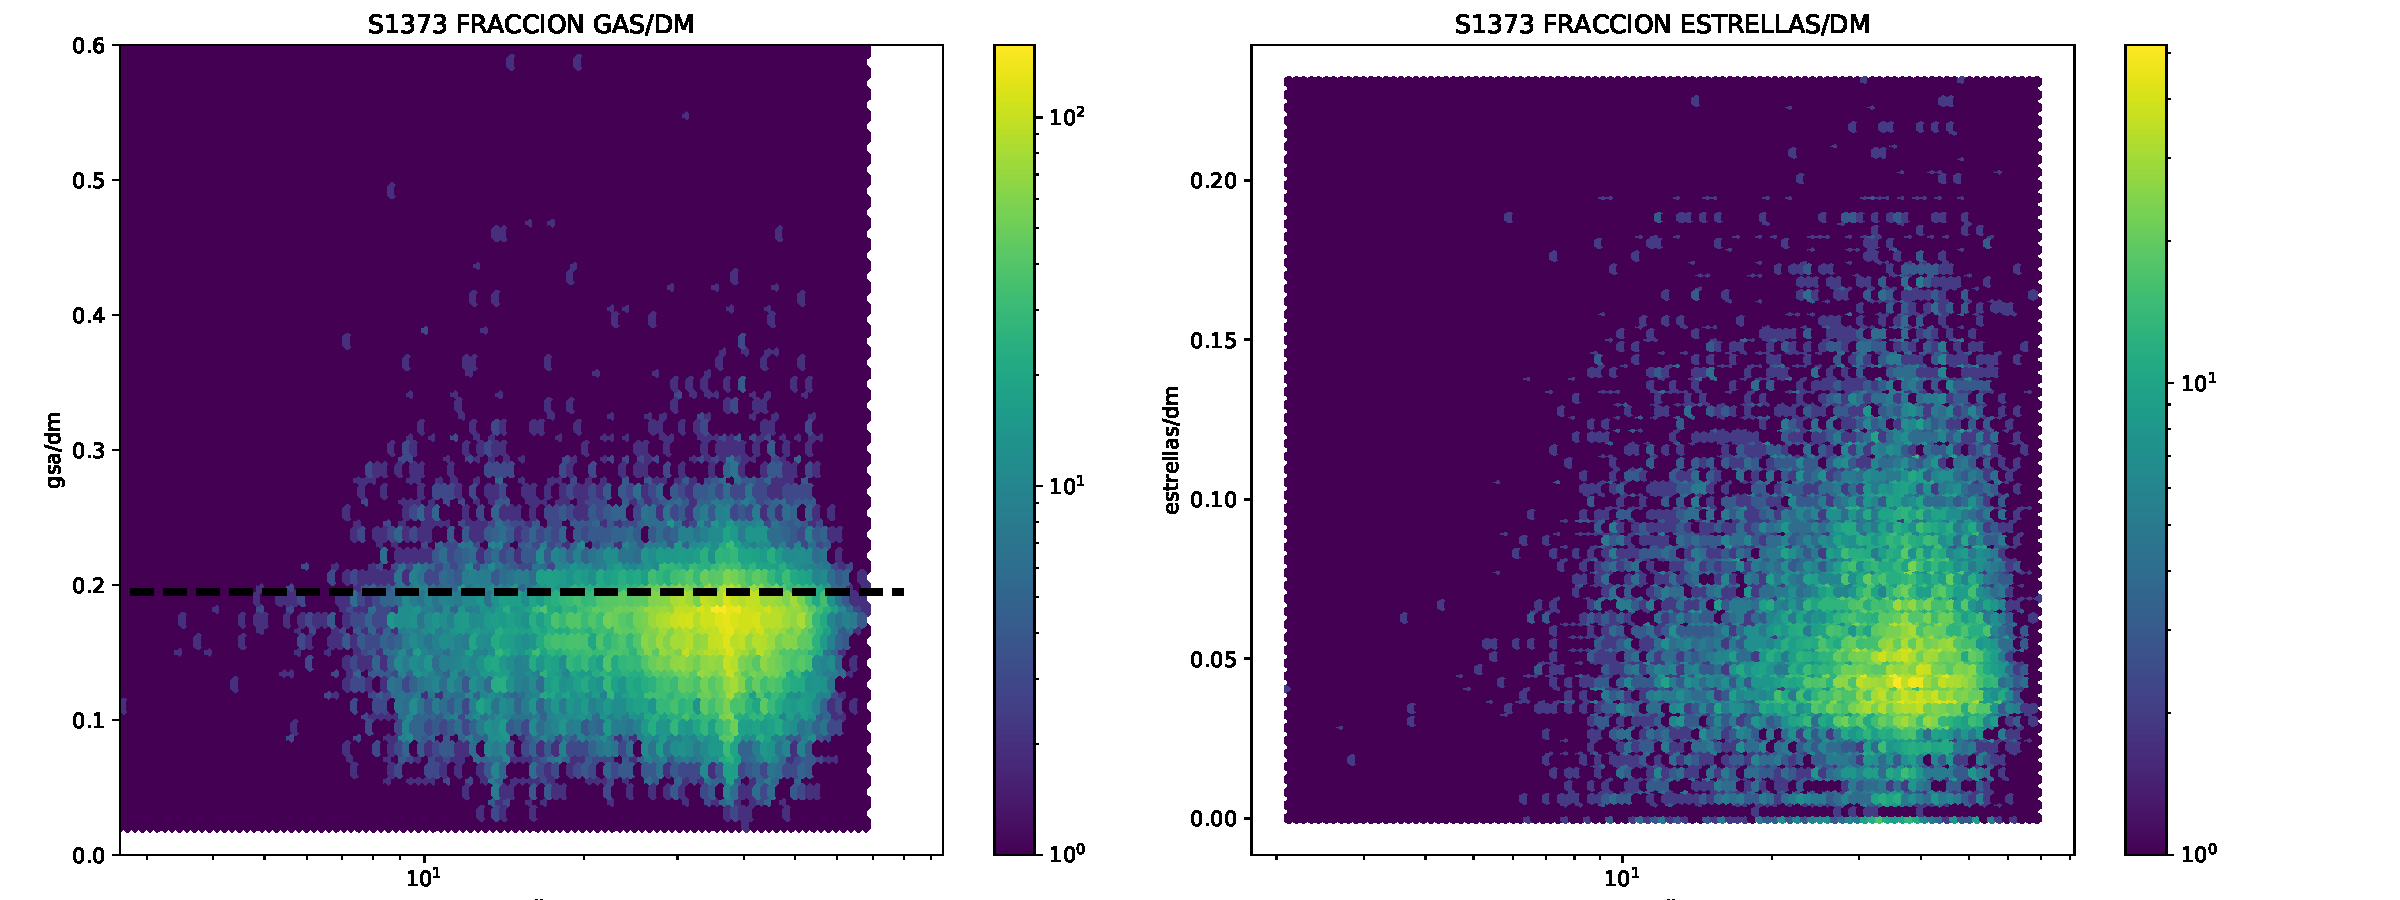
\includegraphics[width=18cm]{Figures/S1373_scatterFRACCIONES2.pdf}
\decoRule
\caption[S1373 GAS/DM perfil (scatter)]{El SPH considera las 32 ? particulas mas cercanas para calcular el hsml, entonces un halo que tenga al menos 32 particulas de gas va a tener sus 23 vecinas en el halo (casi seguro) entonces la masa de gas de ese halo van a ser todas las particulas en el (IZQUIERDA). A unn halos con menos de 32 particulas de gas, le va a pasar que sus particulas de gas van a tener masa FUERA del halo DERECHA).}
\label{fig:Electron}
\end{figure}








\begin{figure}[h]
\centering
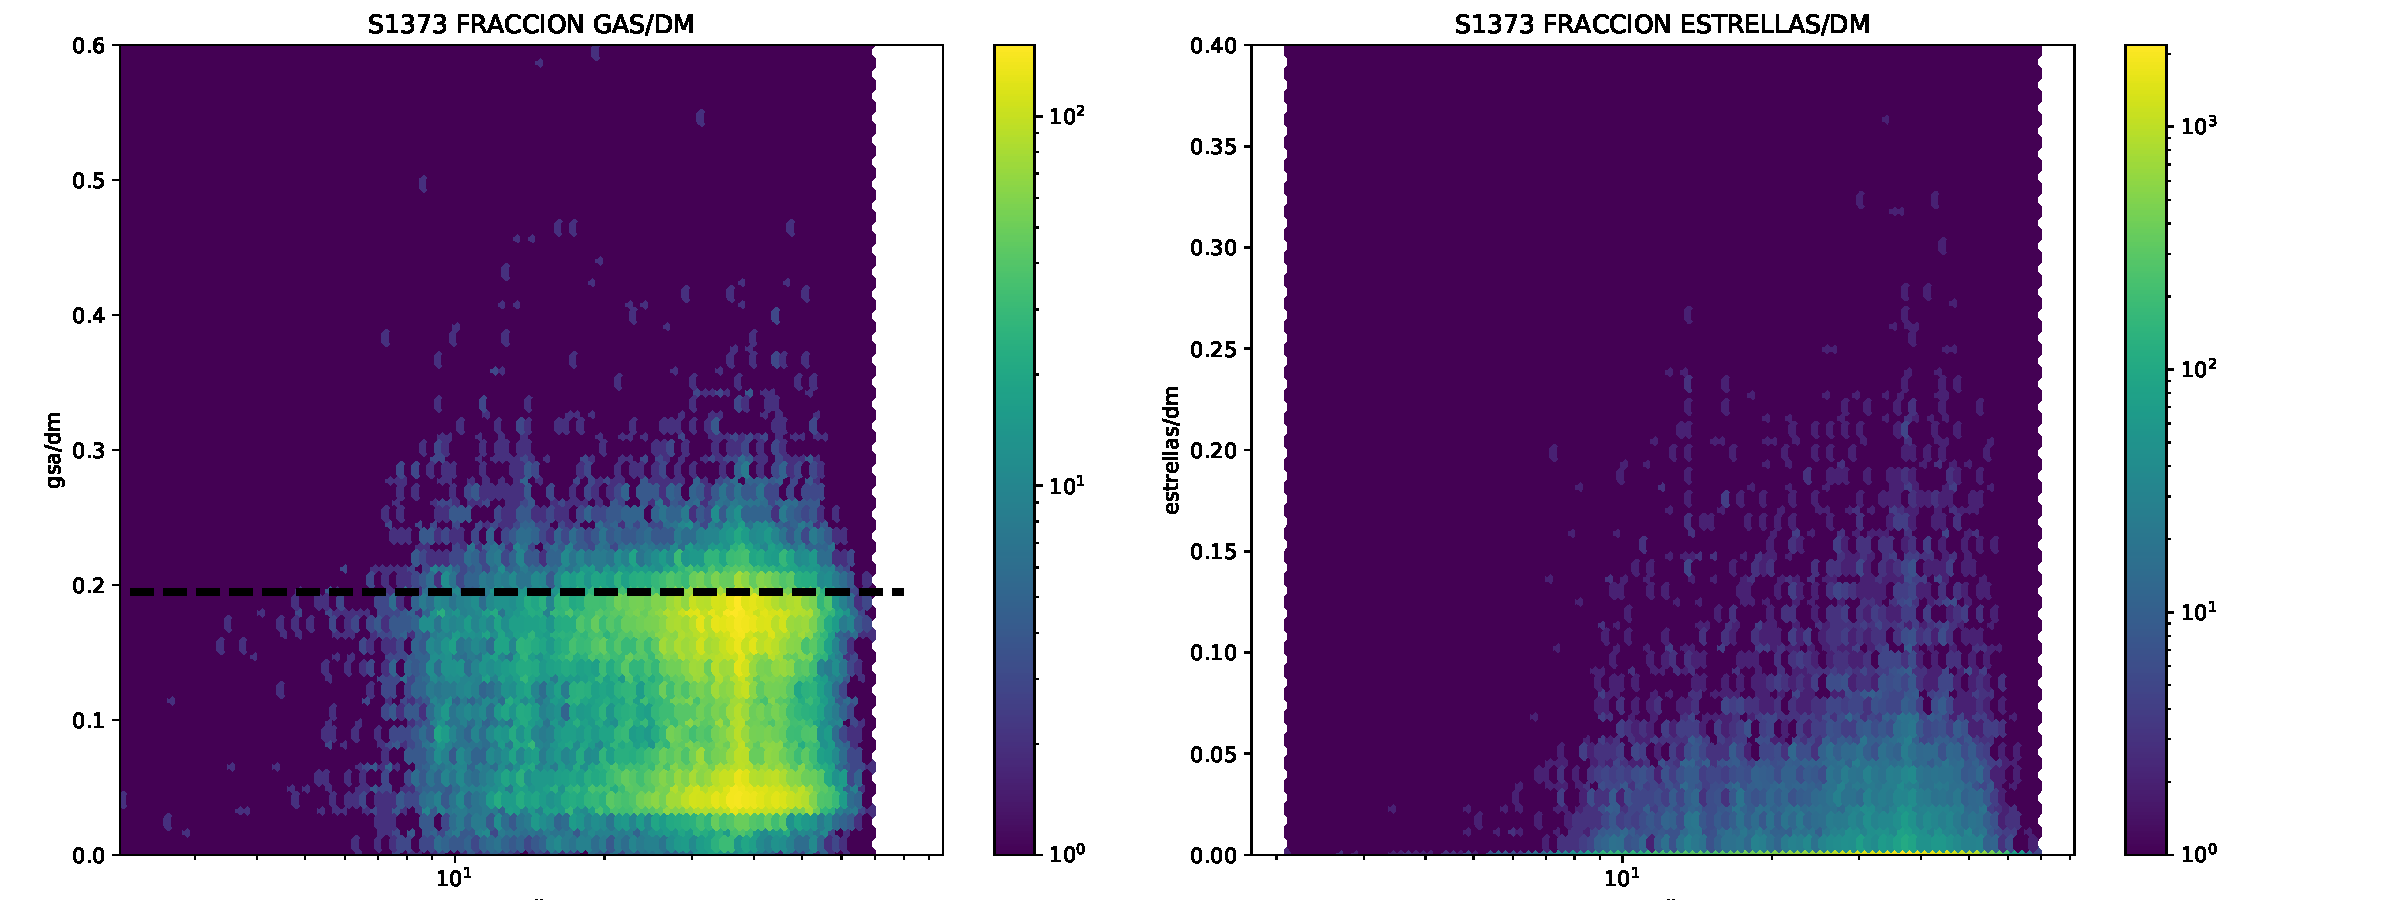
\includegraphics[width=18cm]{Figures/S1373_scatterFRACCIONES.pdf}
\decoRule
\caption[S1373 GAS/DM perfil (scatter)]{Fraccion de gas sobre DM en funcion del centro del void, tamaño del void $\sim$ 9.5 Mpc. A la derecha la fraccion es de Estrellas sobre DM}
\label{fig:Electron}
\end{figure}

\begin{figure}[h]
\centering
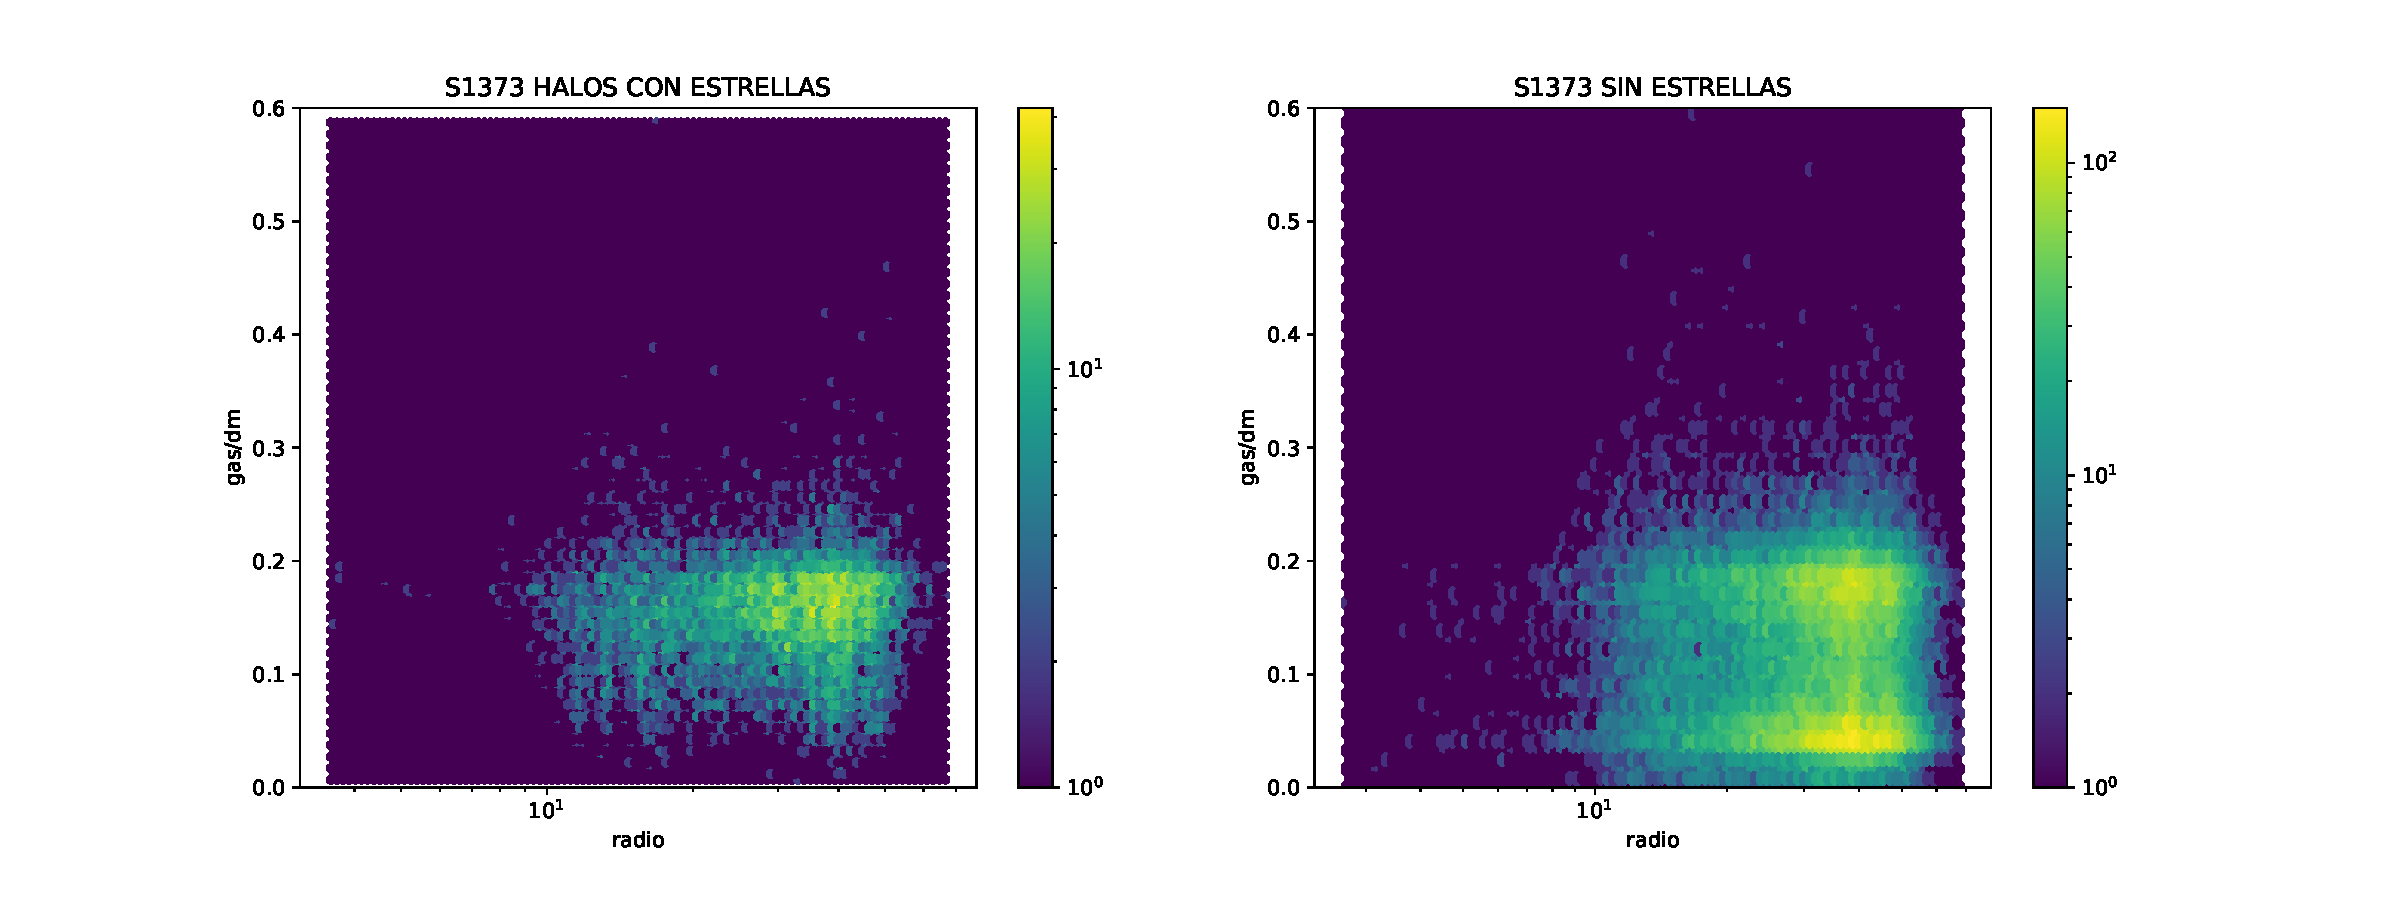
\includegraphics[width=18cm]{Figures/S1373_scatterFRACCIONES_con&sinEST.pdf}
\decoRule
\caption[R1198 GAS/DM perfil (scatter) con y sin estrellas]{Perfil de gas/dm para los halos. A  la izquierda estan los halos que contienen al menos una particula de estrellas. A la derehc a los que no tienen ninguna estrella}
\label{fig:Electron}
\end{figure}

\begin{figure}[h]
\centering
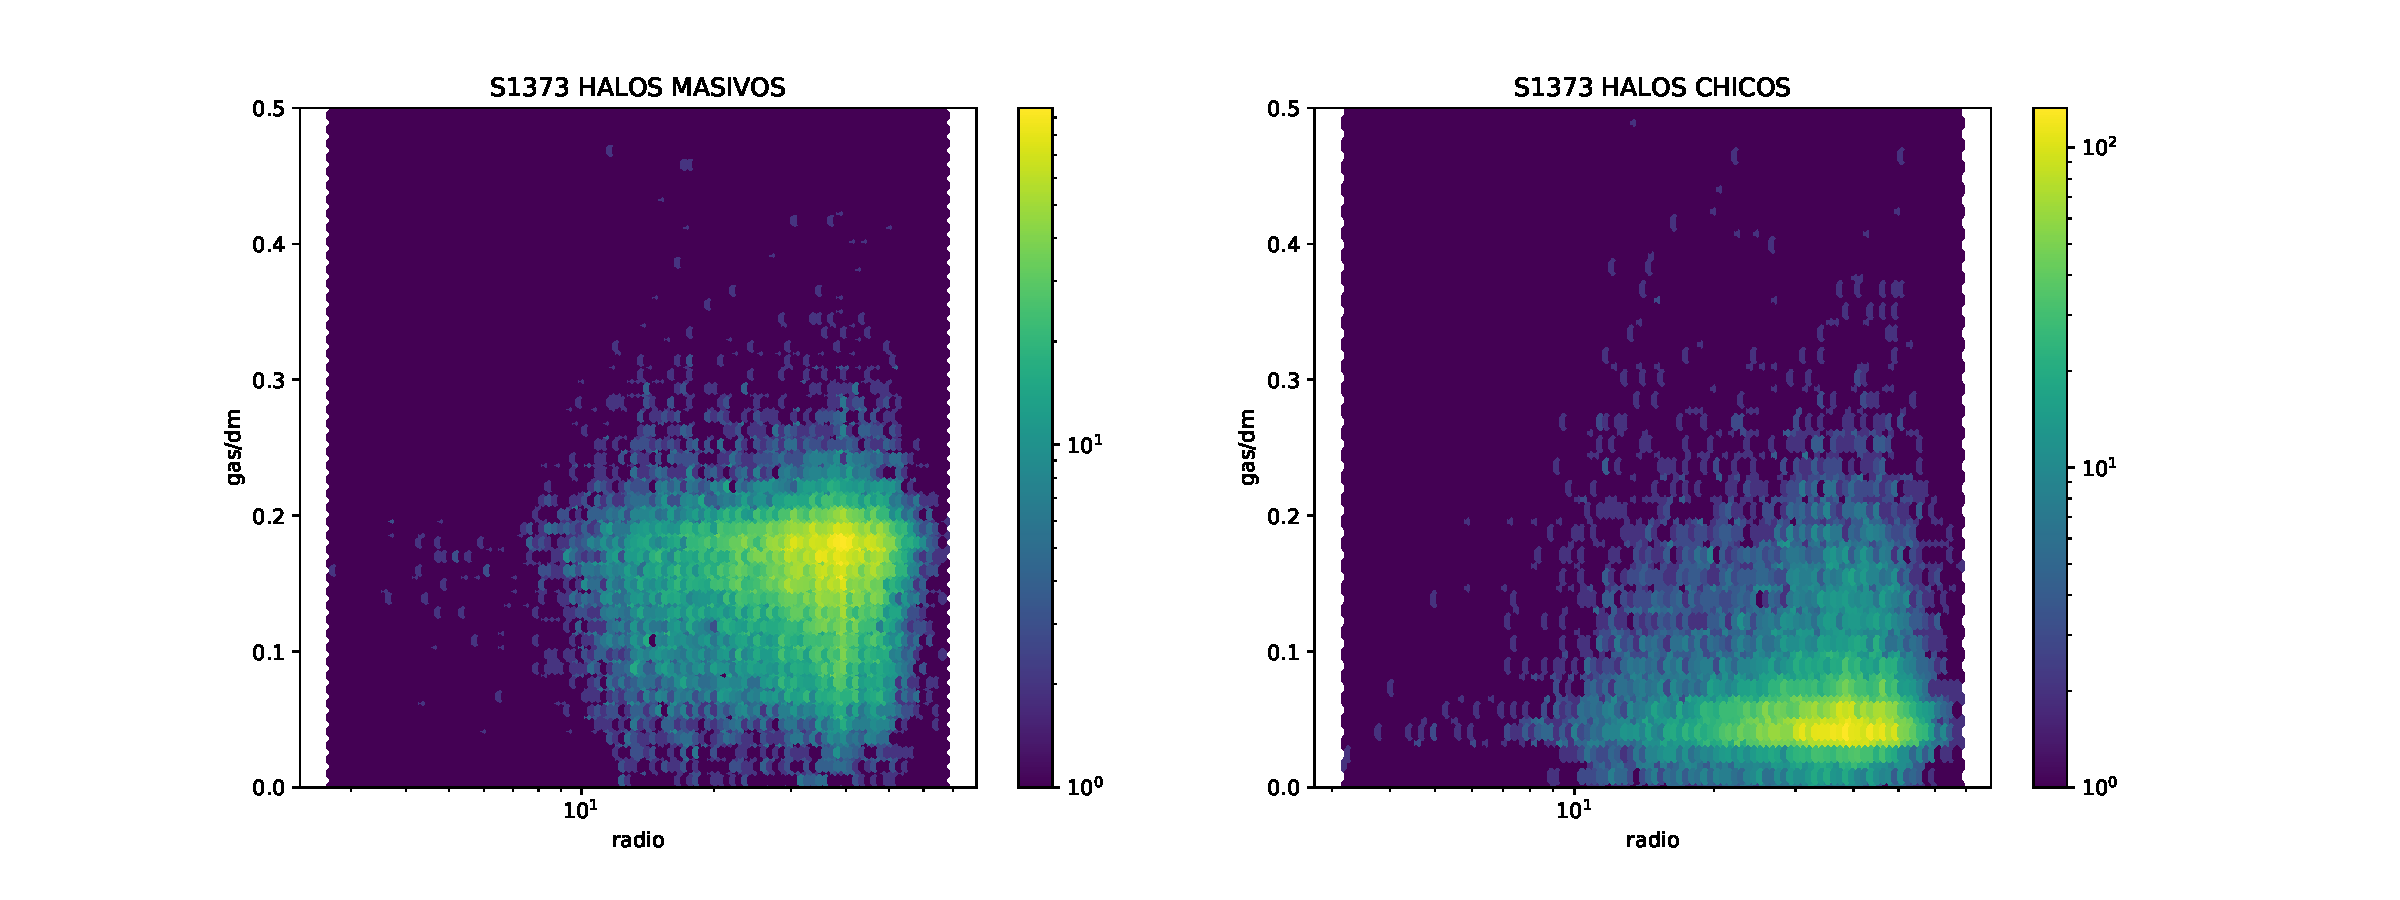
\includegraphics[width=18cm]{Figures/S1373_scatterFRACCIONES_grandesYchicos.pdf}
\decoRule
\caption[R1198 GAS/DM perfil (scatter) halos grandes y chicos]{fraccion de gas sobre DM separando los halos por tamaño. Los halos GRANDES tienen mas de 50 particulas de DM, los chicos menos de 50. }
\label{fig:Electron}
\end{figure}


% Chapter 1

\chapter{DIAGRAMAS DE FASE} % Main chapter title

(paper Shuiyao Huang et al. 2019) 



Most of these
gas particles lie on a well-defined curve in the phase diagram,
which is established by a balance between adiabatic cooling and photoionization heating. A fraction of gas particles are shock heated
when they collapse into the gravitational potential of dark matter
sheets and filaments and are driven into warm-and-hot ionized gas
outside of haloes (upper left) or fall into dark matter haloes and
become hot halo gas (upper right). Radiative cooling later plays a
critical role in the further condensation of gas into the condensed
region (lower right) where SF can occur. In addition, some gas goes
straight from the diffuse to the condensed region, i.e. cold mode
accretion (Keres et al. ˇ 2005, 2009a).



Calcule las fracciones al estilo de Martizzi 2009 y me dio, corte en dens = 2.5 y temp = 5 (la temperatura es el mismo corte, la densidad lo meti a ojo) Me dan muy diferentes. ESTO ES PARA EL VOID S
\begin{figure}[h]
\centering
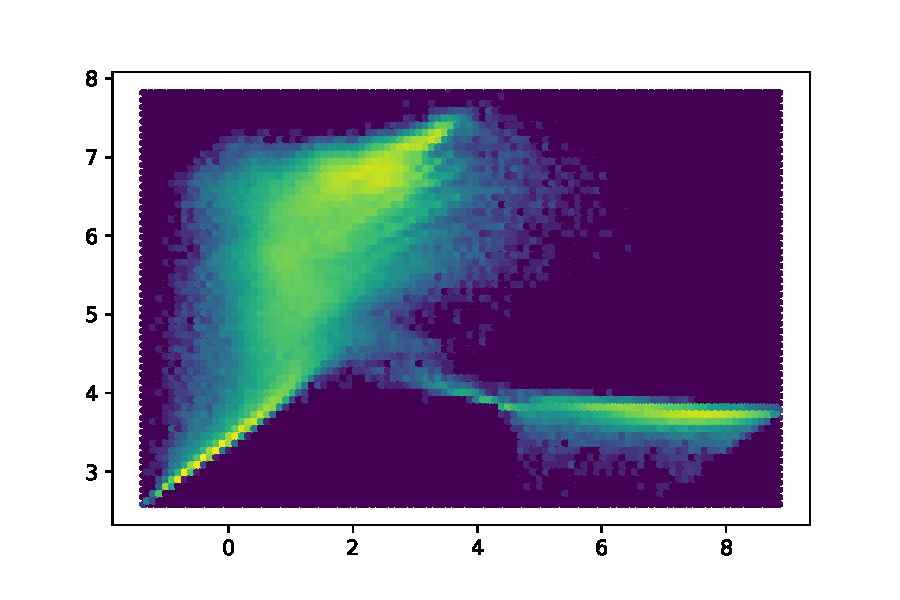
\includegraphics[width=14cm]{Figures/S1373_diagfaseVOID.pdf}
\decoRule
\caption[Diagrama de Fase TODAS particulas]{Densidad vs Temperatura considerando las particulas del void r<9.75}
\label{fig:Electron}
\end{figure}


fraccion DIF 0.19707932560856978

fraccion HALO 0.13583764565477252

fraccion WHIM 0.49660098890788423

fraccion WCGM 0.1704743649519073

fraccion SF 7.674876866194279e-06
\label{Chapter2} % For referencing the chapter elsewhere, use \ref{Chapter1} 

%----------------------------------------------------------------------------------------

% Define some commands to keep the formatting separated from the content 

%----------------------------------------------------------------------------------------
\section{R1198}

\begin{figure}[h]
\centering
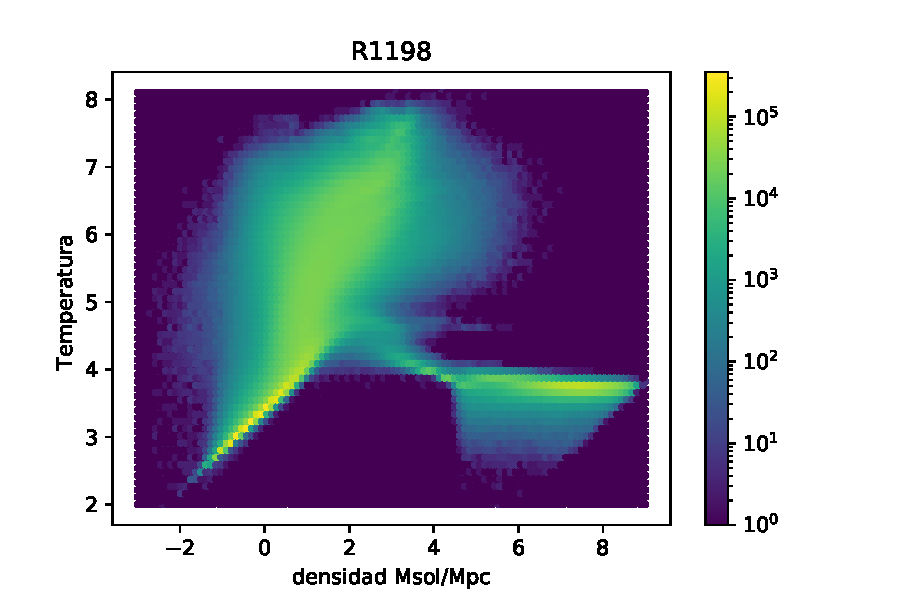
\includegraphics[width=18cm]{Figures/R1198_diagfase.pdf}
\decoRule
\caption[Diagrama de Fase TODAS particulas]{Densidad vs Temperatura considerando todas las particulas $\sim$ 33 millones}
\label{fig:Electron}
\end{figure}

\begin{figure}[h]
\centering
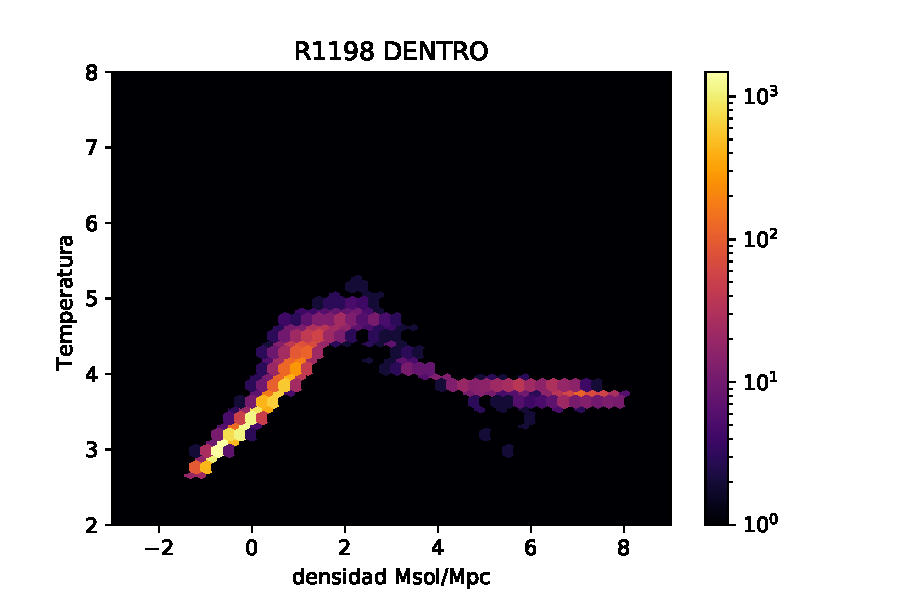
\includegraphics[width=18cm]{Figures/R1198_diagfase_int.pdf}
\decoRule
\caption[Diagrama de Fase R internas]{particulas dentro de un radio de 6 mpc}
\label{fig:Electron}
\end{figure}
\begin{figure}[h]
\centering
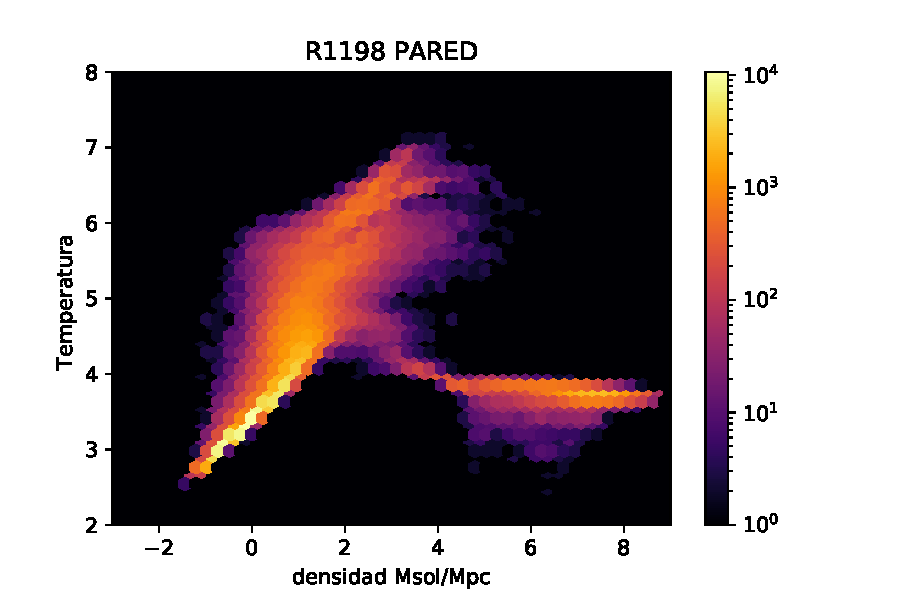
\includegraphics[width=18cm]{Figures/R1198_diagfase_wll.pdf}
\decoRule
\caption[Diagrama de Fase R pared]{particulas entre 6 y 12 Mpc}
\label{fig:Electron}
\end{figure}
\begin{figure}[h]
\centering
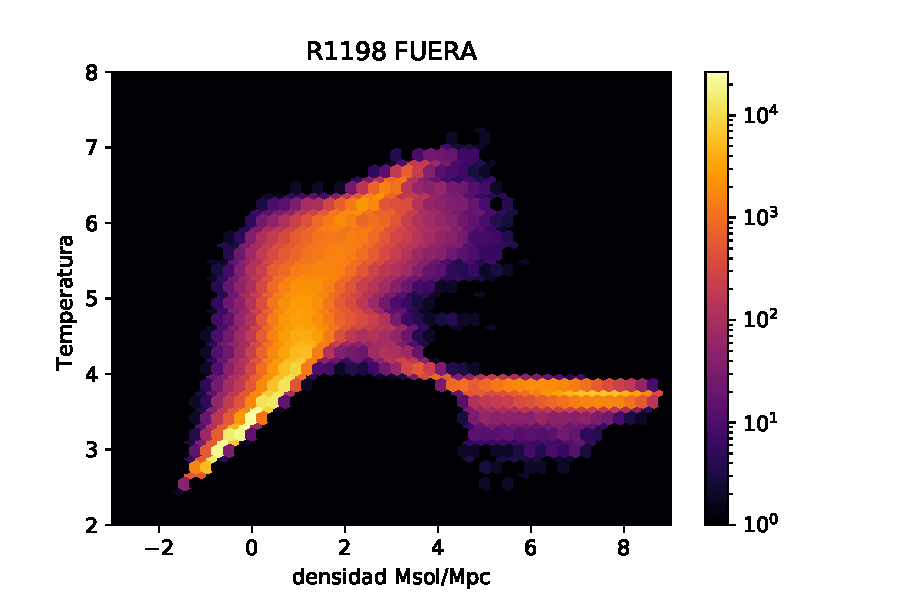
\includegraphics[width=18cm]{Figures/R1198_diagfase_ext.pdf}
\decoRule
\caption[Diagrama de Fase R externas]{particulas entre 12 y 18 Mpc}
\label{fig:Electron}
\end{figure}




\section{S1373}

\begin{figure}[h]
\centering
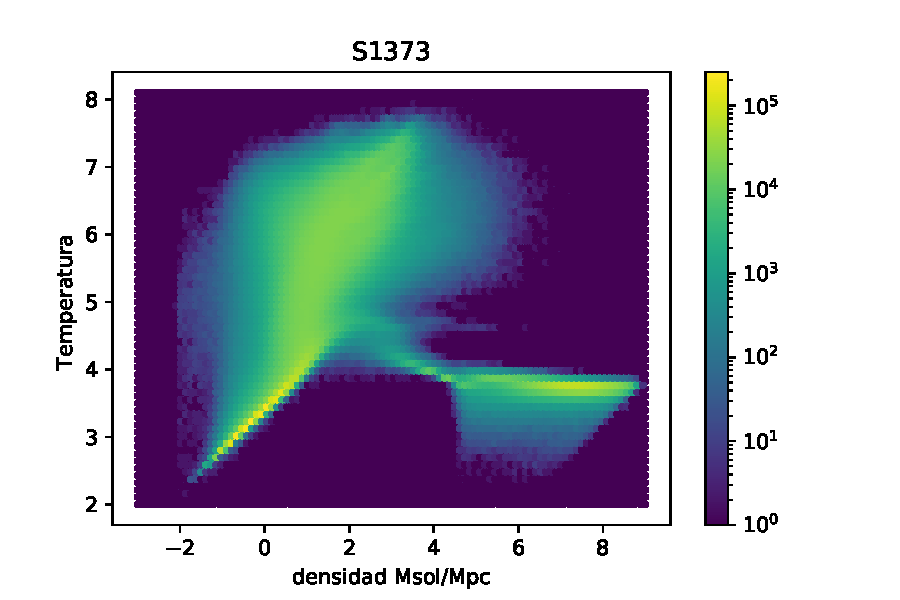
\includegraphics[width=18cm]{Figures/S1373_diagfase.pdf}
\decoRule
\caption[Diagrama de Fase TODAS particulas]{Densidad vs Temperatura considerando todas las particulas $\sim$ 33 millones}
\label{fig:Electron}
\end{figure}



\begin{figure}[h]
\centering
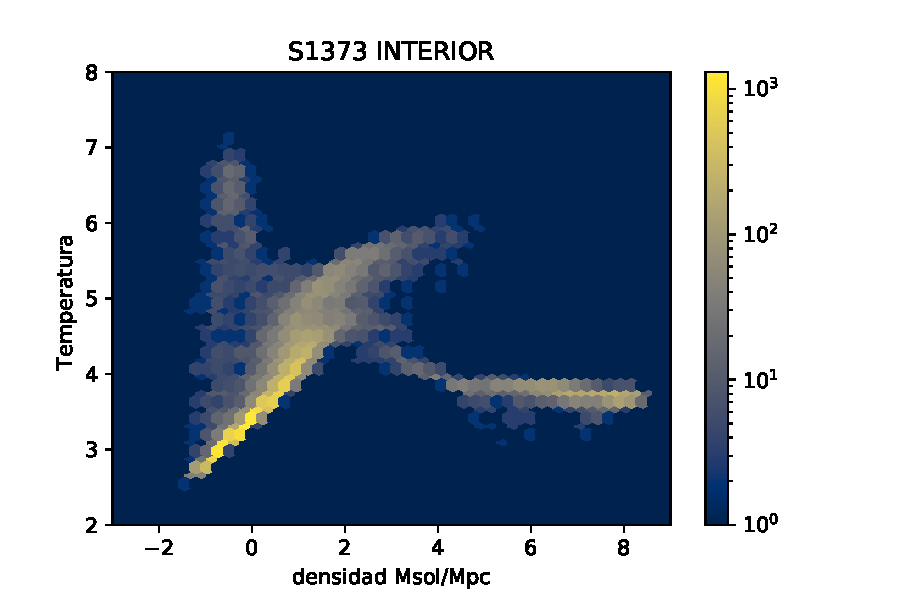
\includegraphics[width=18cm]{Figures/S1373_diagfase_int.pdf}
\decoRule
\caption[Diagrama de Fase S internas]{particulas dentro de un radio de 6 mpc}
\label{fig:Electron}
\end{figure}
\begin{figure}[h]
\centering
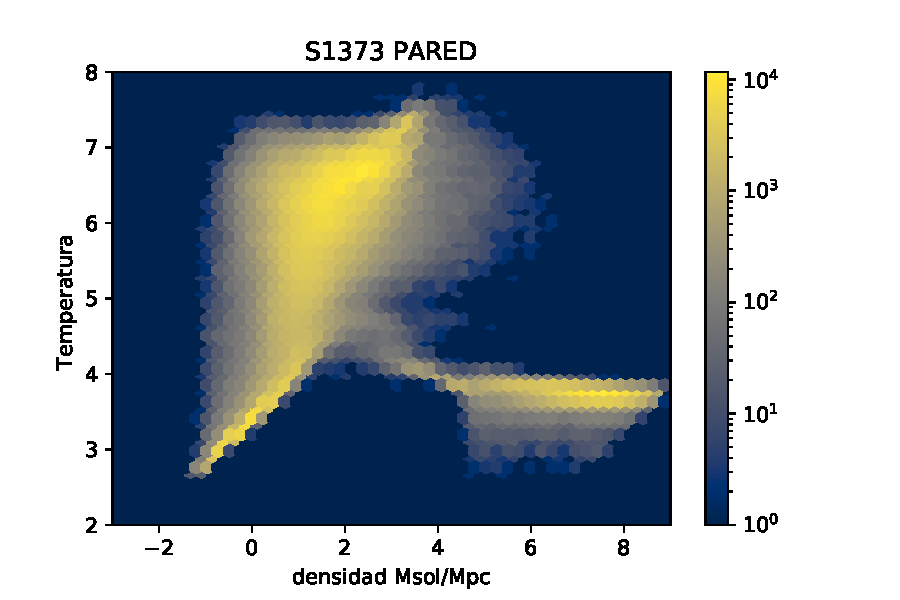
\includegraphics[width=18cm]{Figures/S1373_diagfase_wll.pdf}
\decoRule
\caption[Diagrama de Fase S pared]{particulas entre 6 y 12 Mpc}
\label{fig:Electron}
\end{figure}
\begin{figure}[h]
\centering
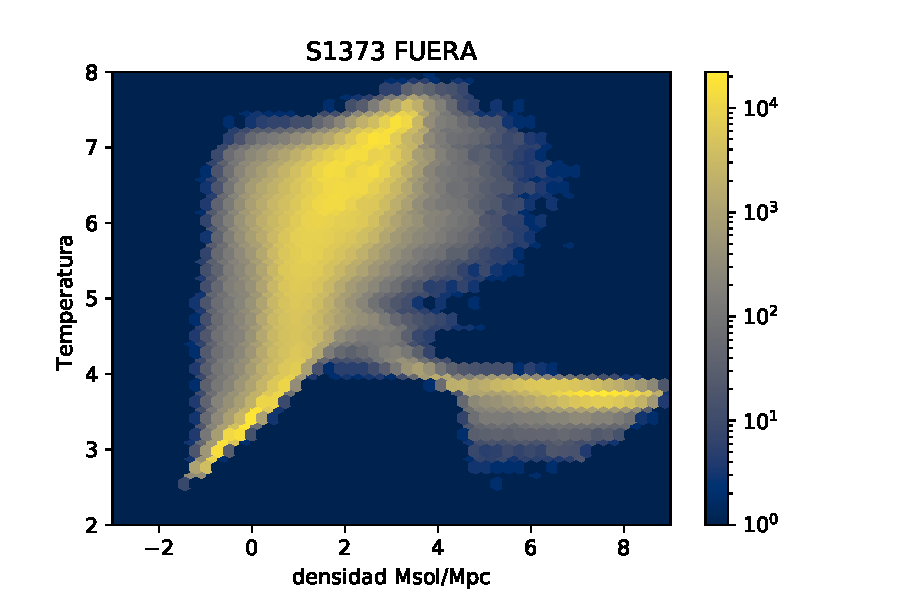
\includegraphics[width=18cm]{Figures/S1373_diagfase_ext.pdf}
\decoRule
\caption[Diagrama de Fase S externas]{particulas entre 12 y 18 Mpc}
\label{fig:Electron}
\end{figure} 
\chapter{look back time}

Agarre el Void S mas alla de el radio de void (15 < r > 25) donde la densidad es mas parecida que a la del universo  e hice los diagramas de fase a diferentes redshift. 

\begin{figure}[h]
\centering
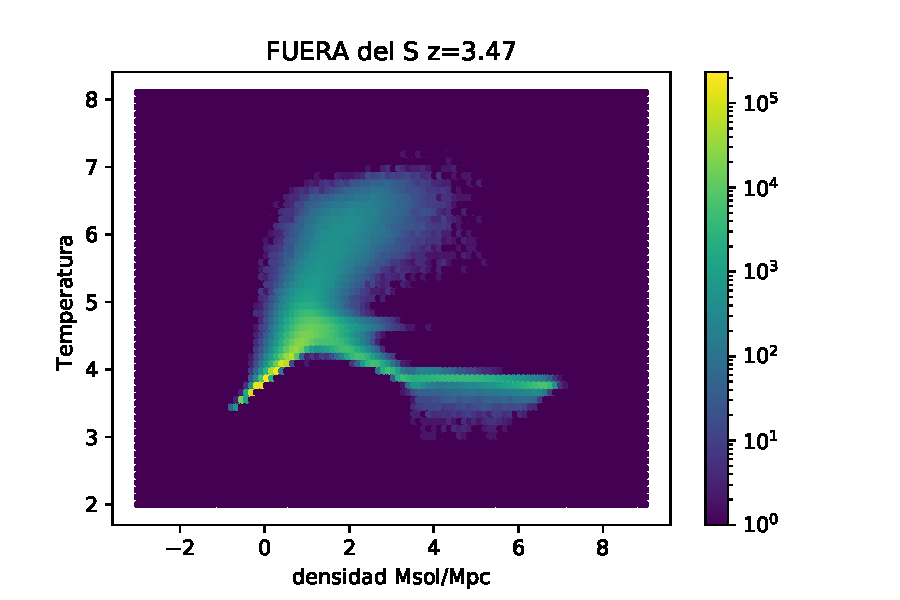
\includegraphics[width=18cm]{Figures/S_df_s25.pdf}
\decoRule
\caption[Fraccione stellar vs gas]{Fracciones de gs/dm vs estrellas/dm }
\label{fig:Electron}
\end{figure}

\begin{figure}[h]
\centering
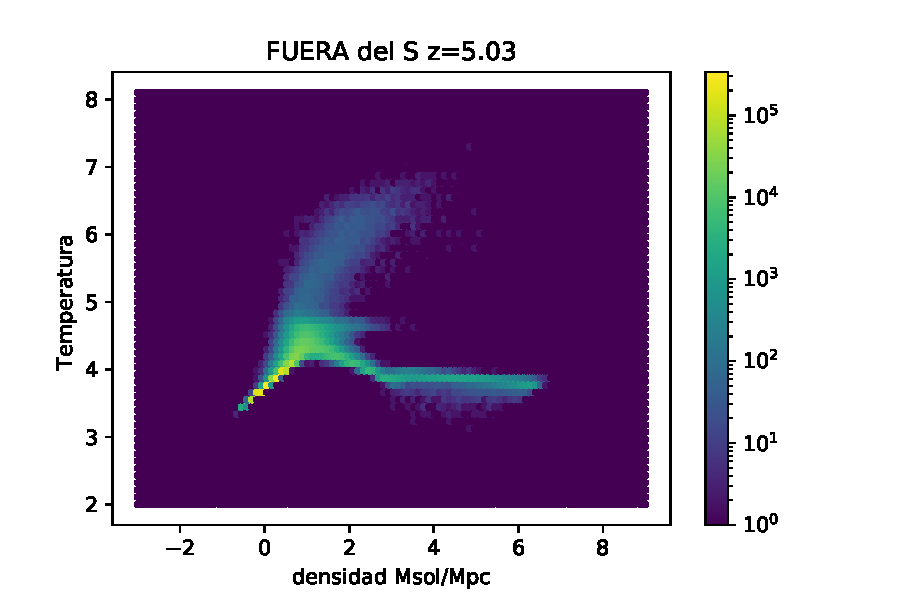
\includegraphics[width=18cm]{Figures/S_df_s20.pdf}
\decoRule
\caption[Fraccione stellar vs gas]{Fracciones de gs/dm vs estrellas/dm }
\label{fig:Electron}
\end{figure}

\begin{figure}[h]
\centering
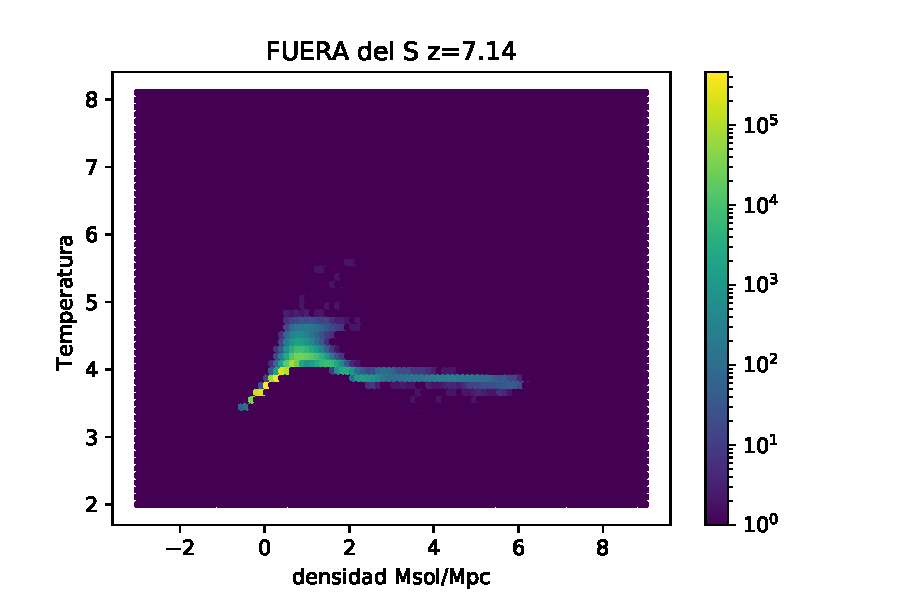
\includegraphics[width=18cm]{Figures/S_df_s15.pdf}
\decoRule
\caption[Fraccione stellar vs gas]{Fracciones de gs/dm vs estrellas/dm }
\label{fig:Electron}
\end{figure}
\chapter{4}


\begin{figure}[h]
\centering
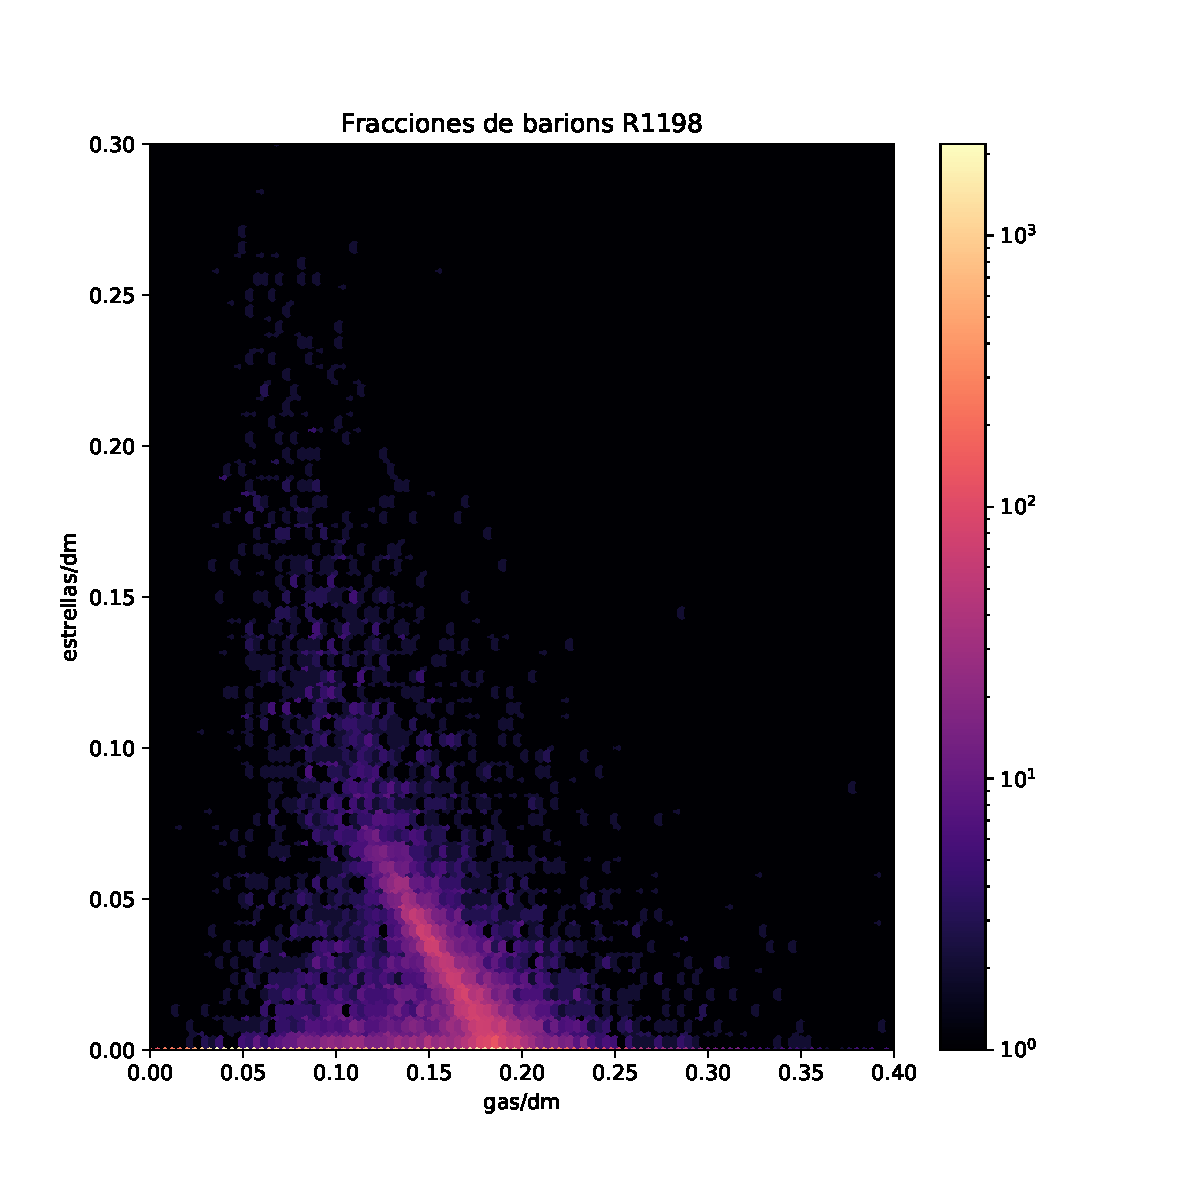
\includegraphics[width=18cm]{Figures/R1198_gas-est_frac.pdf}
\decoRule
\caption[Fraccione stellar vs gas]{Fracciones de gs/dm vs estrellas/dm }
\label{fig:Electron}
\end{figure}

\begin{figure}[h]
\centering
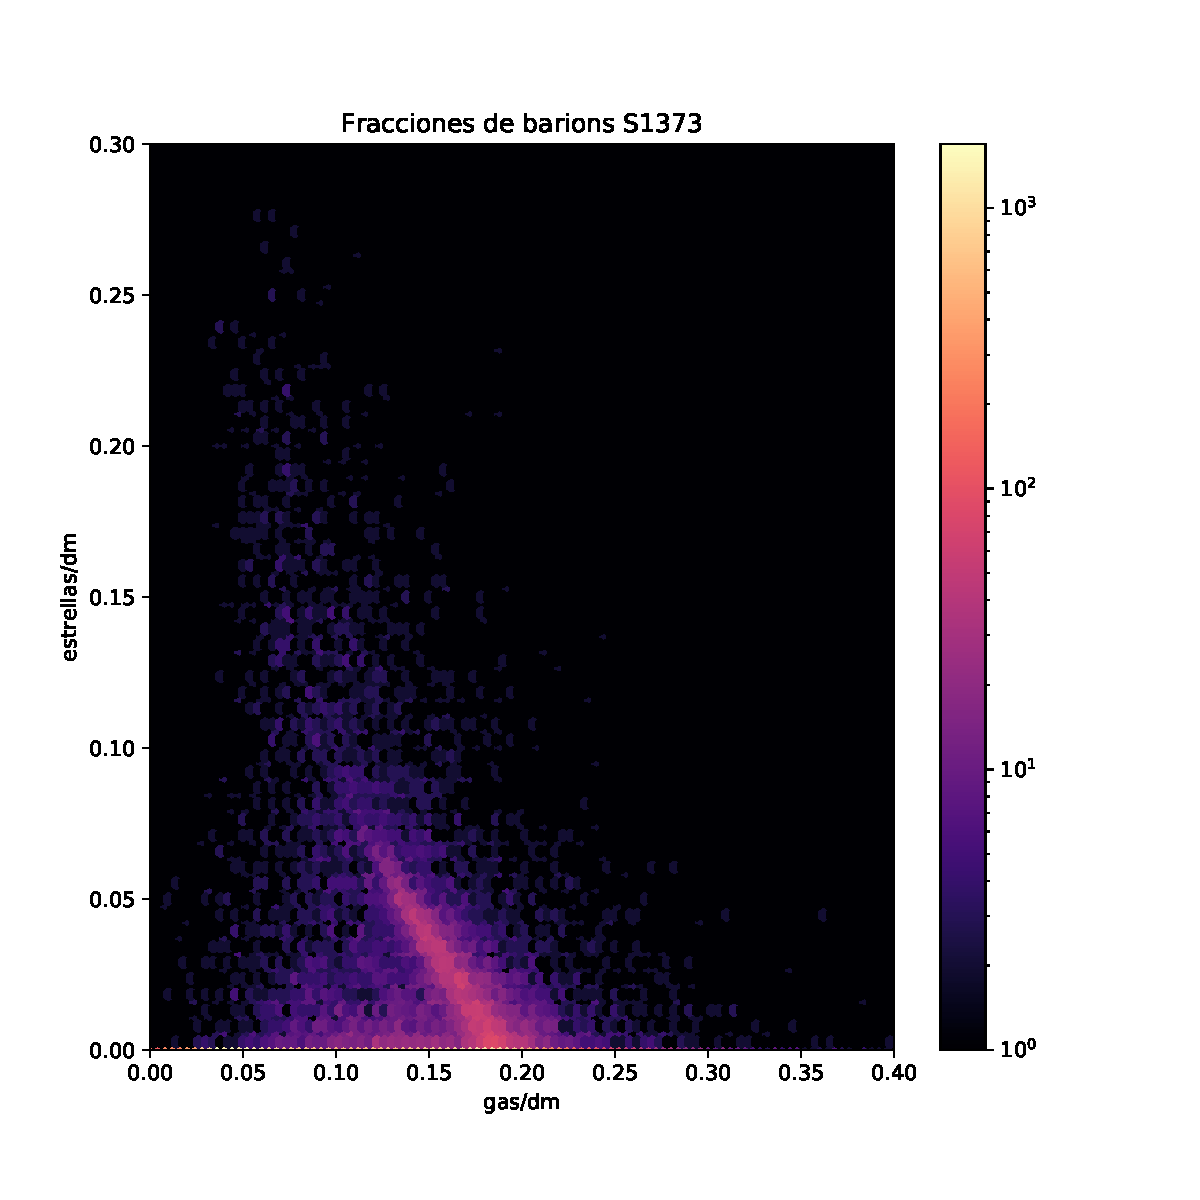
\includegraphics[width=18cm]{Figures/S1373_gas-est_frac.pdf}
\decoRule
\caption[Fraccione stellar vs gas]{Fracciones de gs/dm vs estrellas/dm }
\label{fig:Electron}
\end{figure}

\begin{figure}[h]
\centering
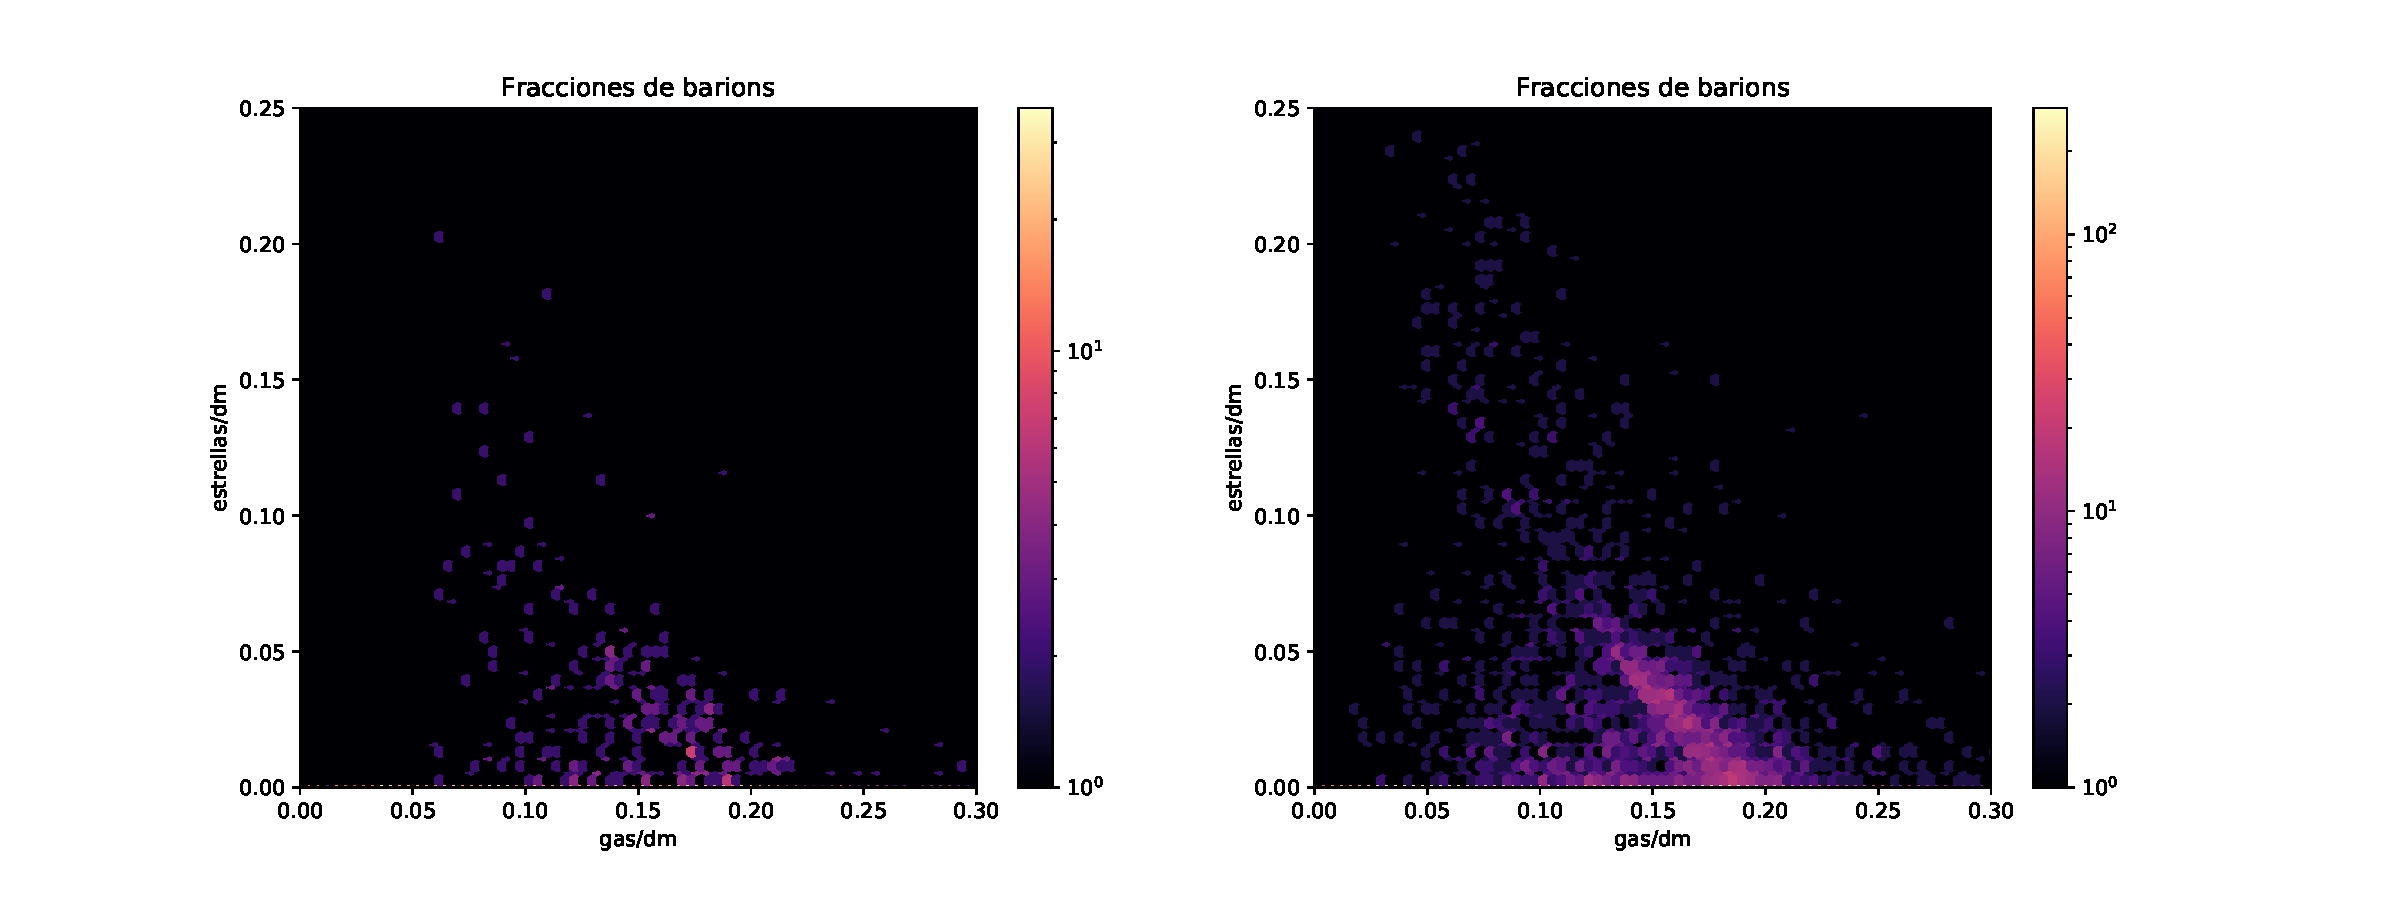
\includegraphics[width=18cm]{Figures/S1373_fraccionesdebarions.pdf}
\decoRule
\caption[Fraccione stellar vs gas]{Fracciones de gs/dm vs estrellas/dm para el VOID (r<10 Mpc y para el entorno r>10}
\label{fig:Electron}
\end{figure}

\begin{figure}[h]
\centering
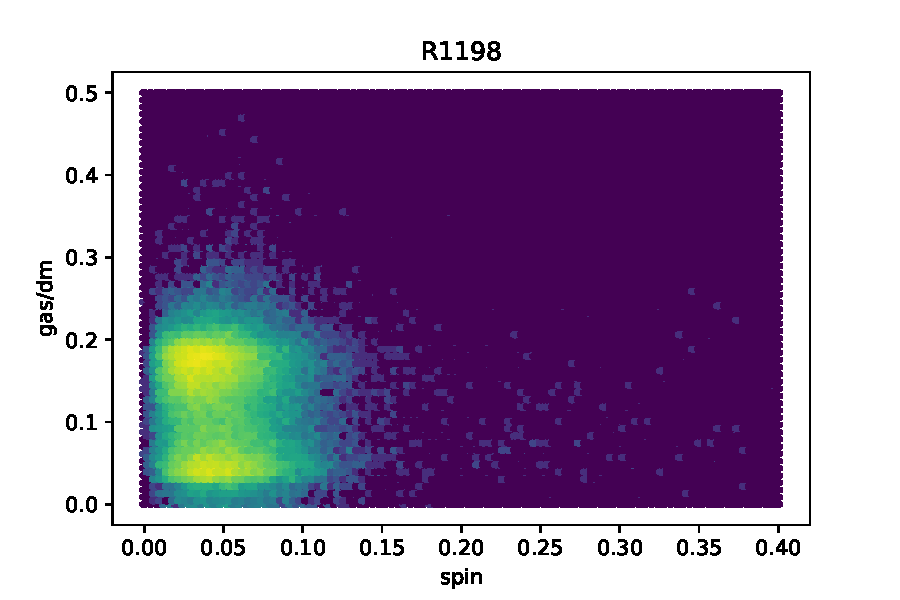
\includegraphics[width=18cm]{Figures/R1198_frac-spin.pdf}
\decoRule
\caption[Fraccione stellar vs gas]{Fracciones de gs/dm vs estrellas/dm para el VOID (r<10 Mpc y para el entorno r>10}
\label{fig:Electron}
\end{figure}

\begin{figure}[h]
\centering
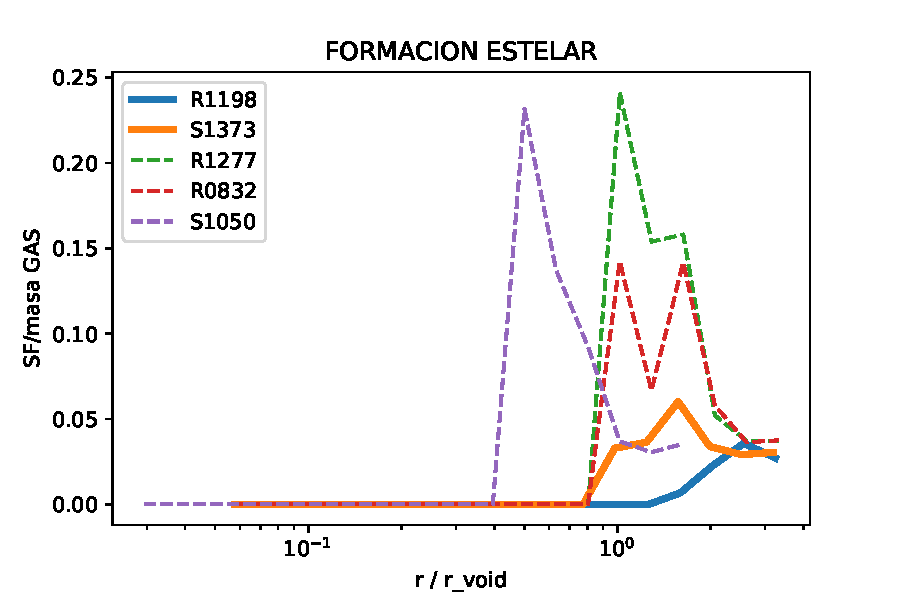
\includegraphics[width=18cm]{Figures/SF.pdf}
\decoRule
\caption[Fraccione stellar vs gas]{Fracciones de gs/dm vs estrellas/dm para el VOID (r<10 Mpc y para el entorno r>10}
\label{fig:Electron}
\end{figure}

\begin{figure}[h]
\centering
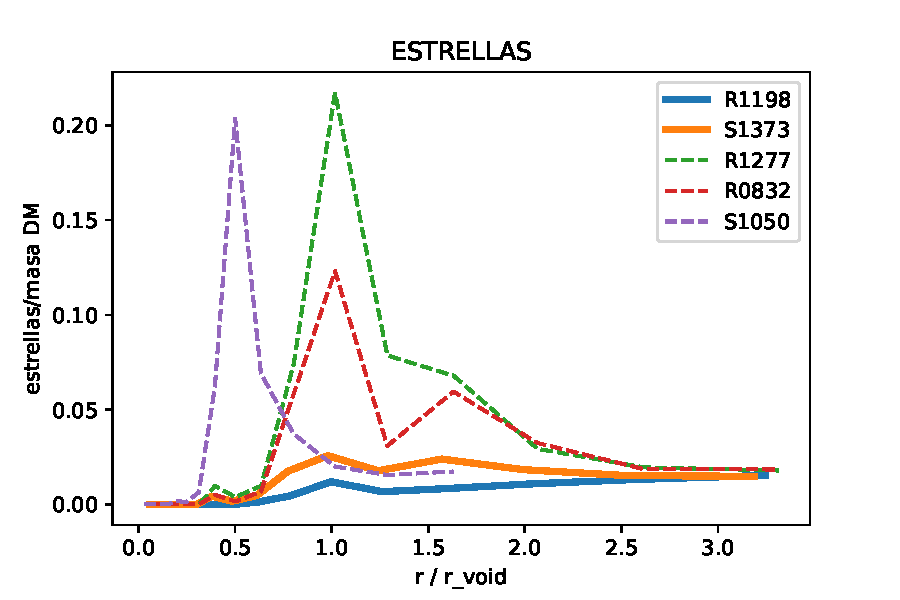
\includegraphics[width=18cm]{Figures/ESTRELLAS.pdf}
\decoRule
\caption[Fraccione stellar vs gas]{Fracciones de gs/dm vs estrellas/dm para el VOID (r<10 Mpc y para el entorno r>10}
\label{fig:Electron}
\end{figure}

\begin{figure}[h]
\centering
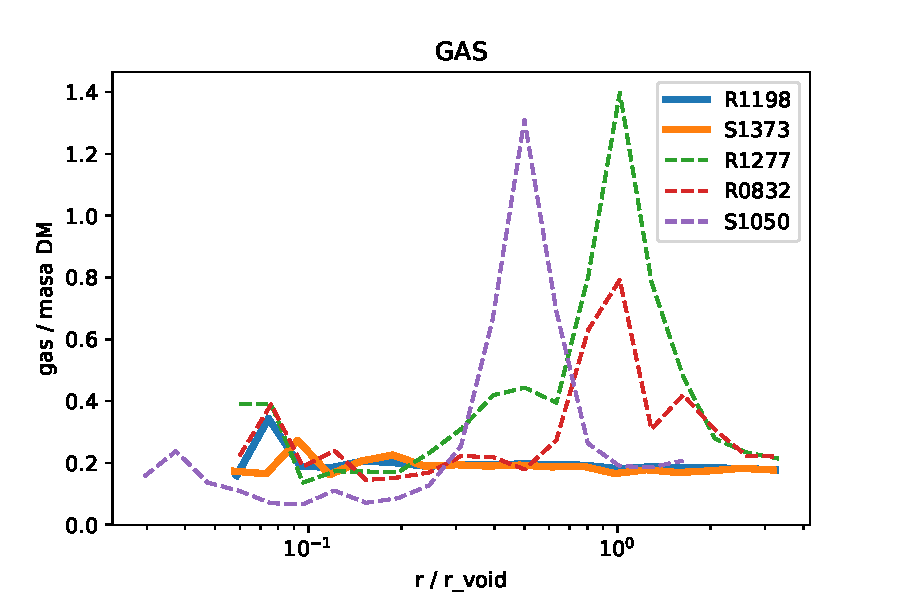
\includegraphics[width=18cm]{Figures/GAS.pdf}
\decoRule
\caption[Fraccione stellar vs gas]{Fracciones de gs/dm vs estrellas/dm para el VOID (r<10 Mpc y para el entorno r>10}
\label{fig:Electron}
\end{figure}

\begin{figure}[h]
\centering
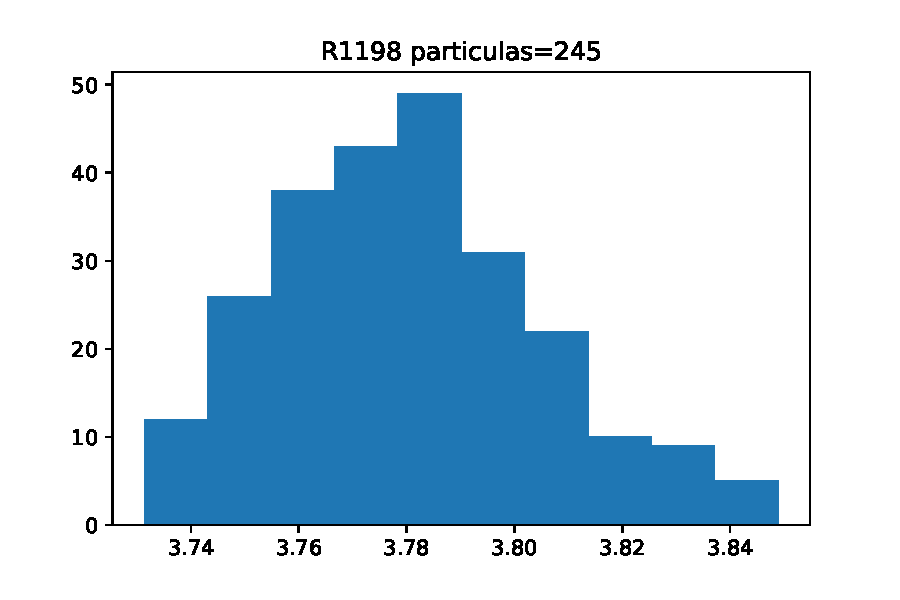
\includegraphics[width=18cm]{Figures/R1198_SFhist.pdf}
\decoRule
\caption[R1198 SF distribucion]{histograma de las 245 particulas de gas con formaci\'on estelar}
\label{fig:Electron}
\end{figure}

\begin{figure}[h]
\centering
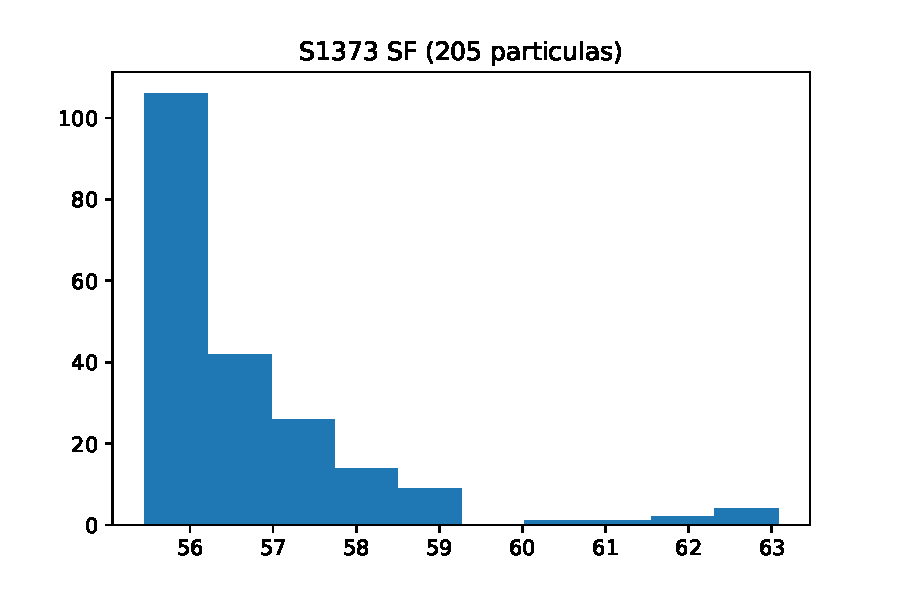
\includegraphics[width=18cm]{Figures/S1373_SFhist.pdf}
\decoRule
\caption[S1373 SF distribucion]{histograma de las 205 particulas de gas con formaci\'on estelar}
\label{fig:Electron}
\end{figure} 
%\chapter{5}

\begin{figure}[h]
\centering
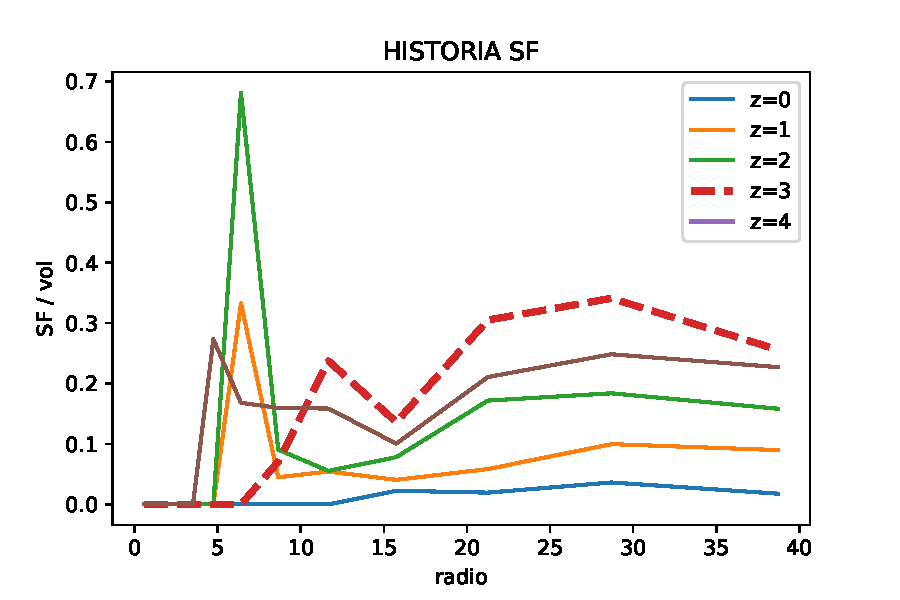
\includegraphics[width=10cm]{Figures/RSF_history.pdf}
\decoRule
\caption[RSF hsitory]{perfil diferencial de formacion estelar a diferentes redshift}
\label{fig:Electron}
\end{figure}

\begin{figure}[h]
\centering
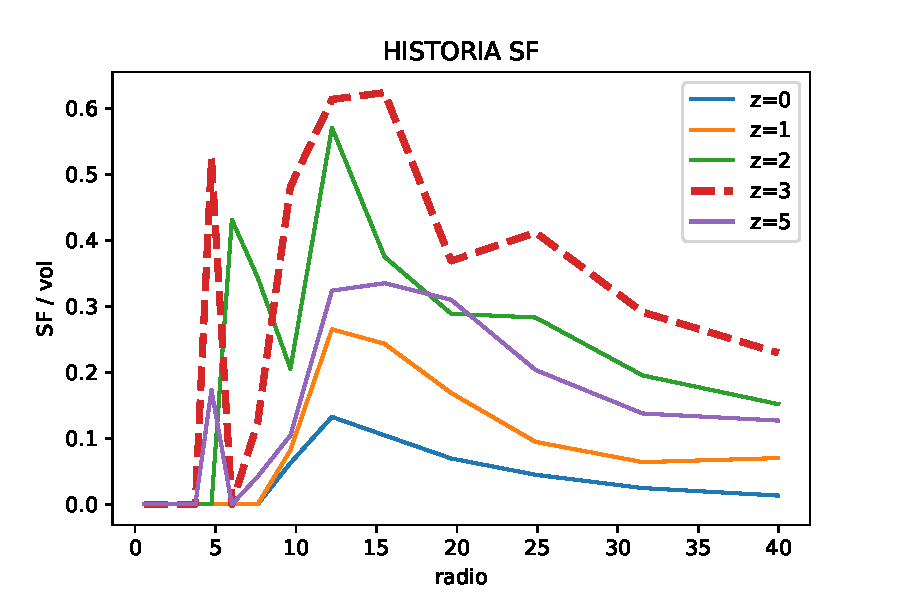
\includegraphics[width=10cm]{Figures/SSF_history.pdf}
\decoRule
\caption[SSF hsitory]{perfil diferencial de formacion estelar a diferentes redshift}
\label{fig:Electron}
\end{figure}

\begin{figure}[h]
\centering
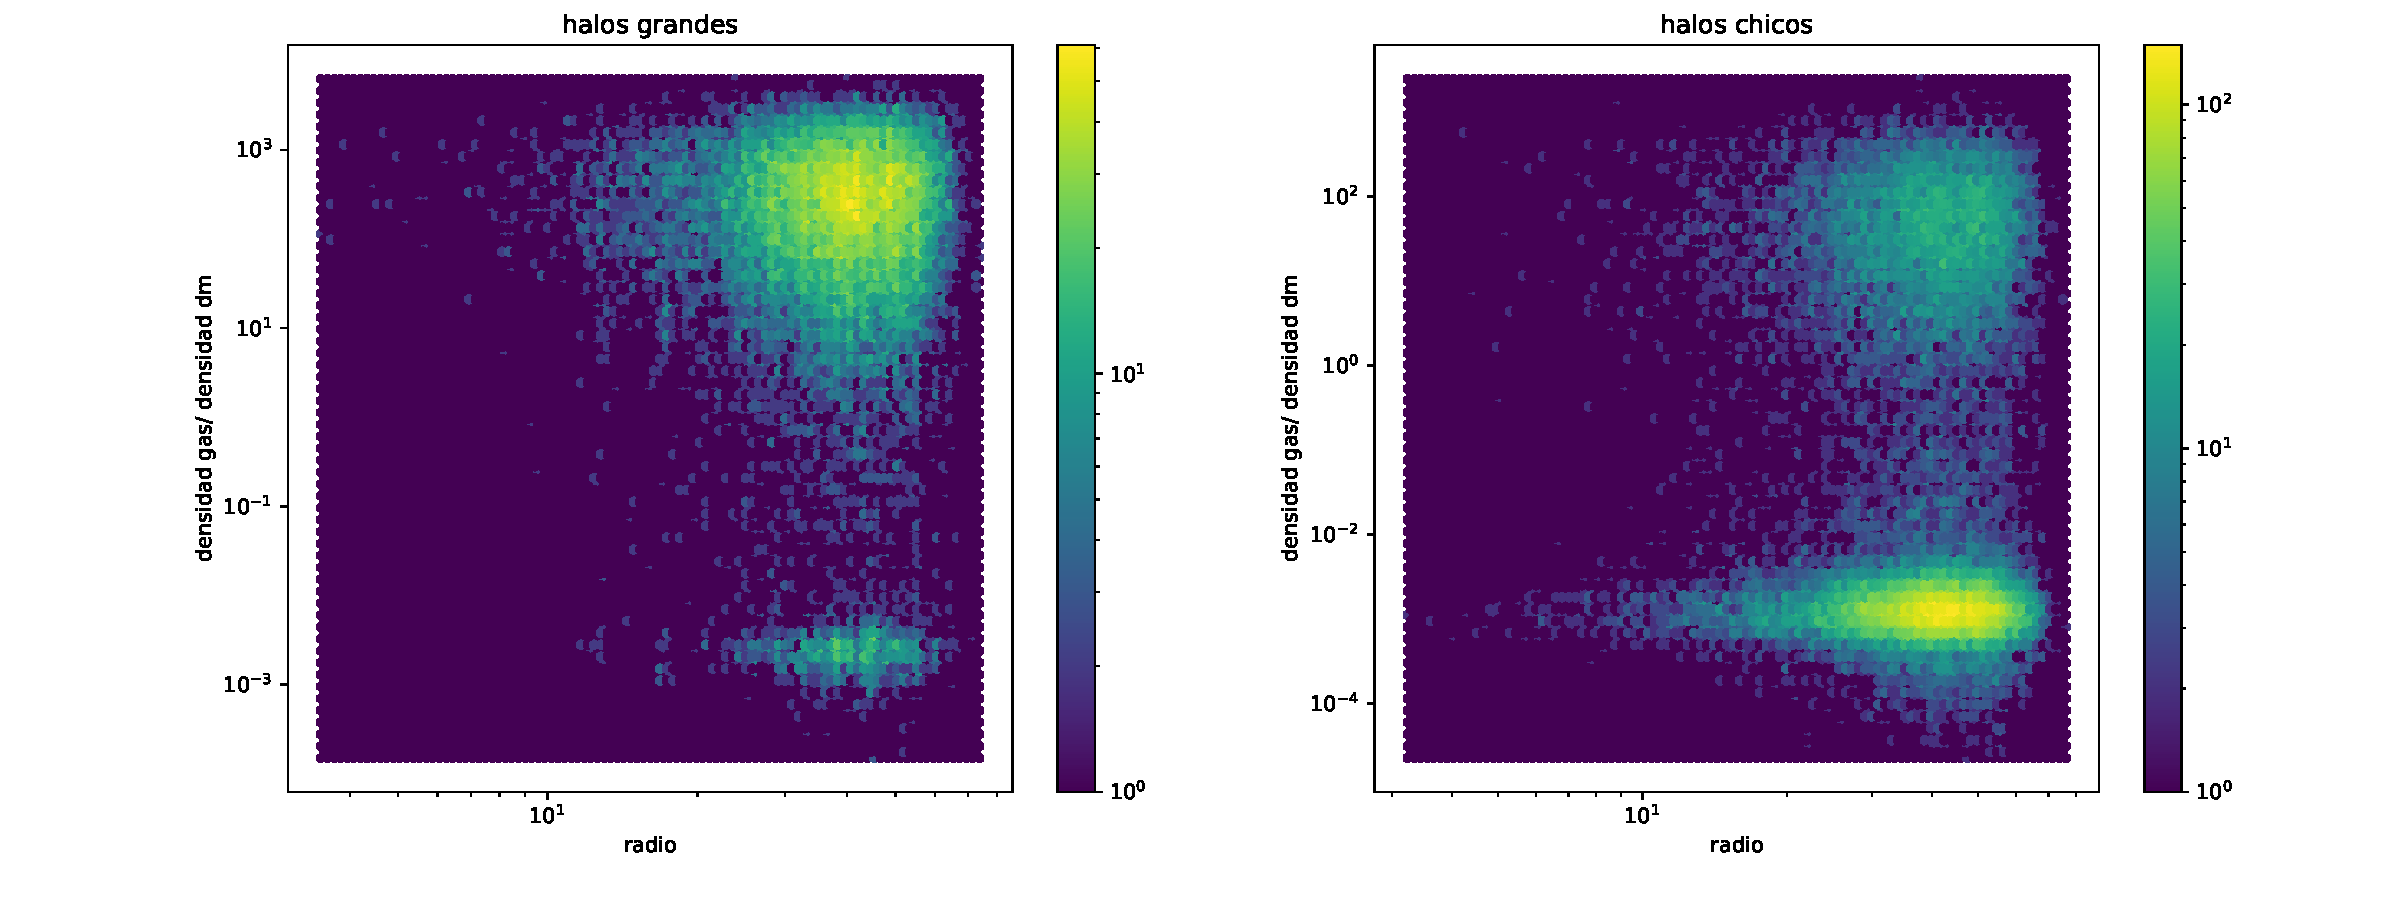
\includegraphics[width=18cm]{Figures/R_sctFRACC1.pdf}
\decoRule
\caption[perfil del void R]{}
\label{fig:Electron}
\end{figure}

\begin{figure}[h]
\centering
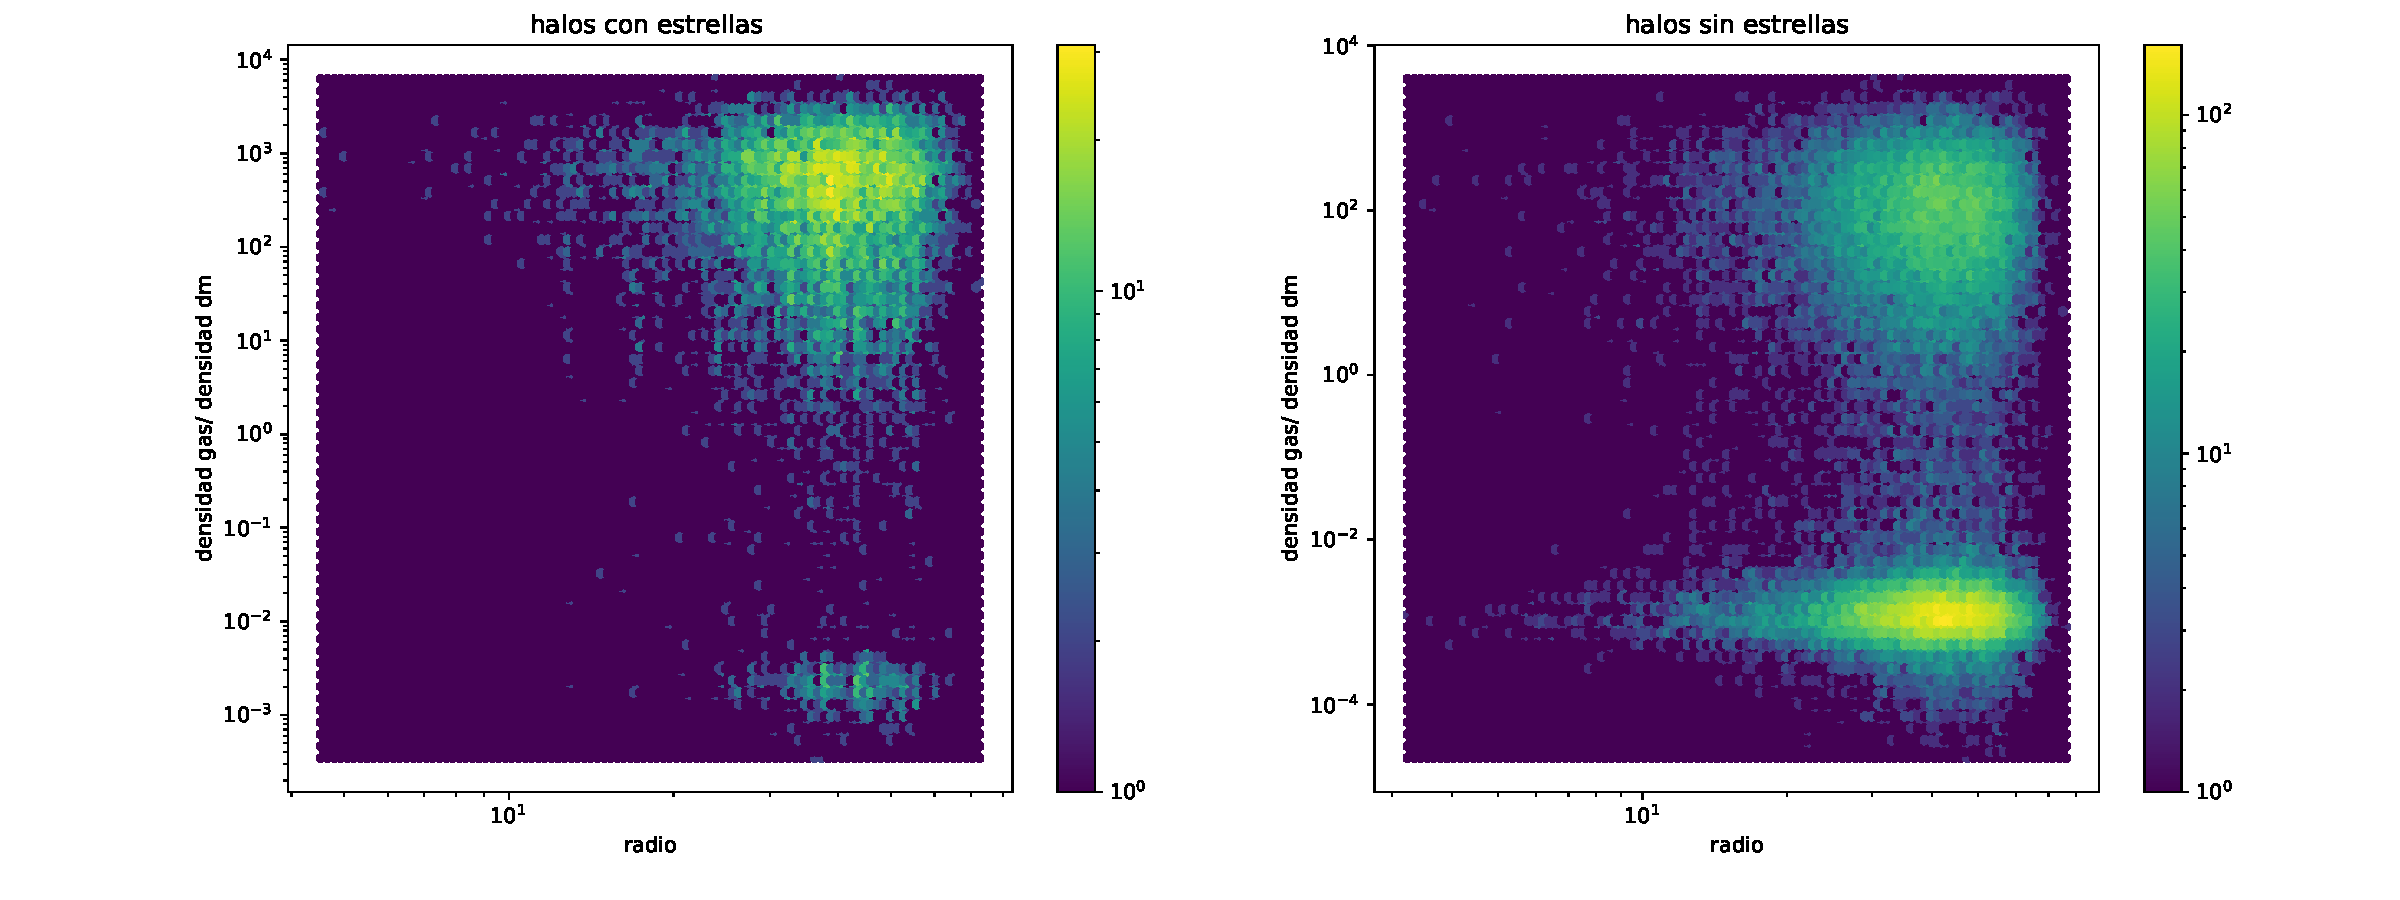
\includegraphics[width=18cm]{Figures/R_sctFRACC2.pdf}
\decoRule
\caption[perfil del void R]{}
\label{fig:Electron}
\end{figure}

\begin{figure}[h]
\centering
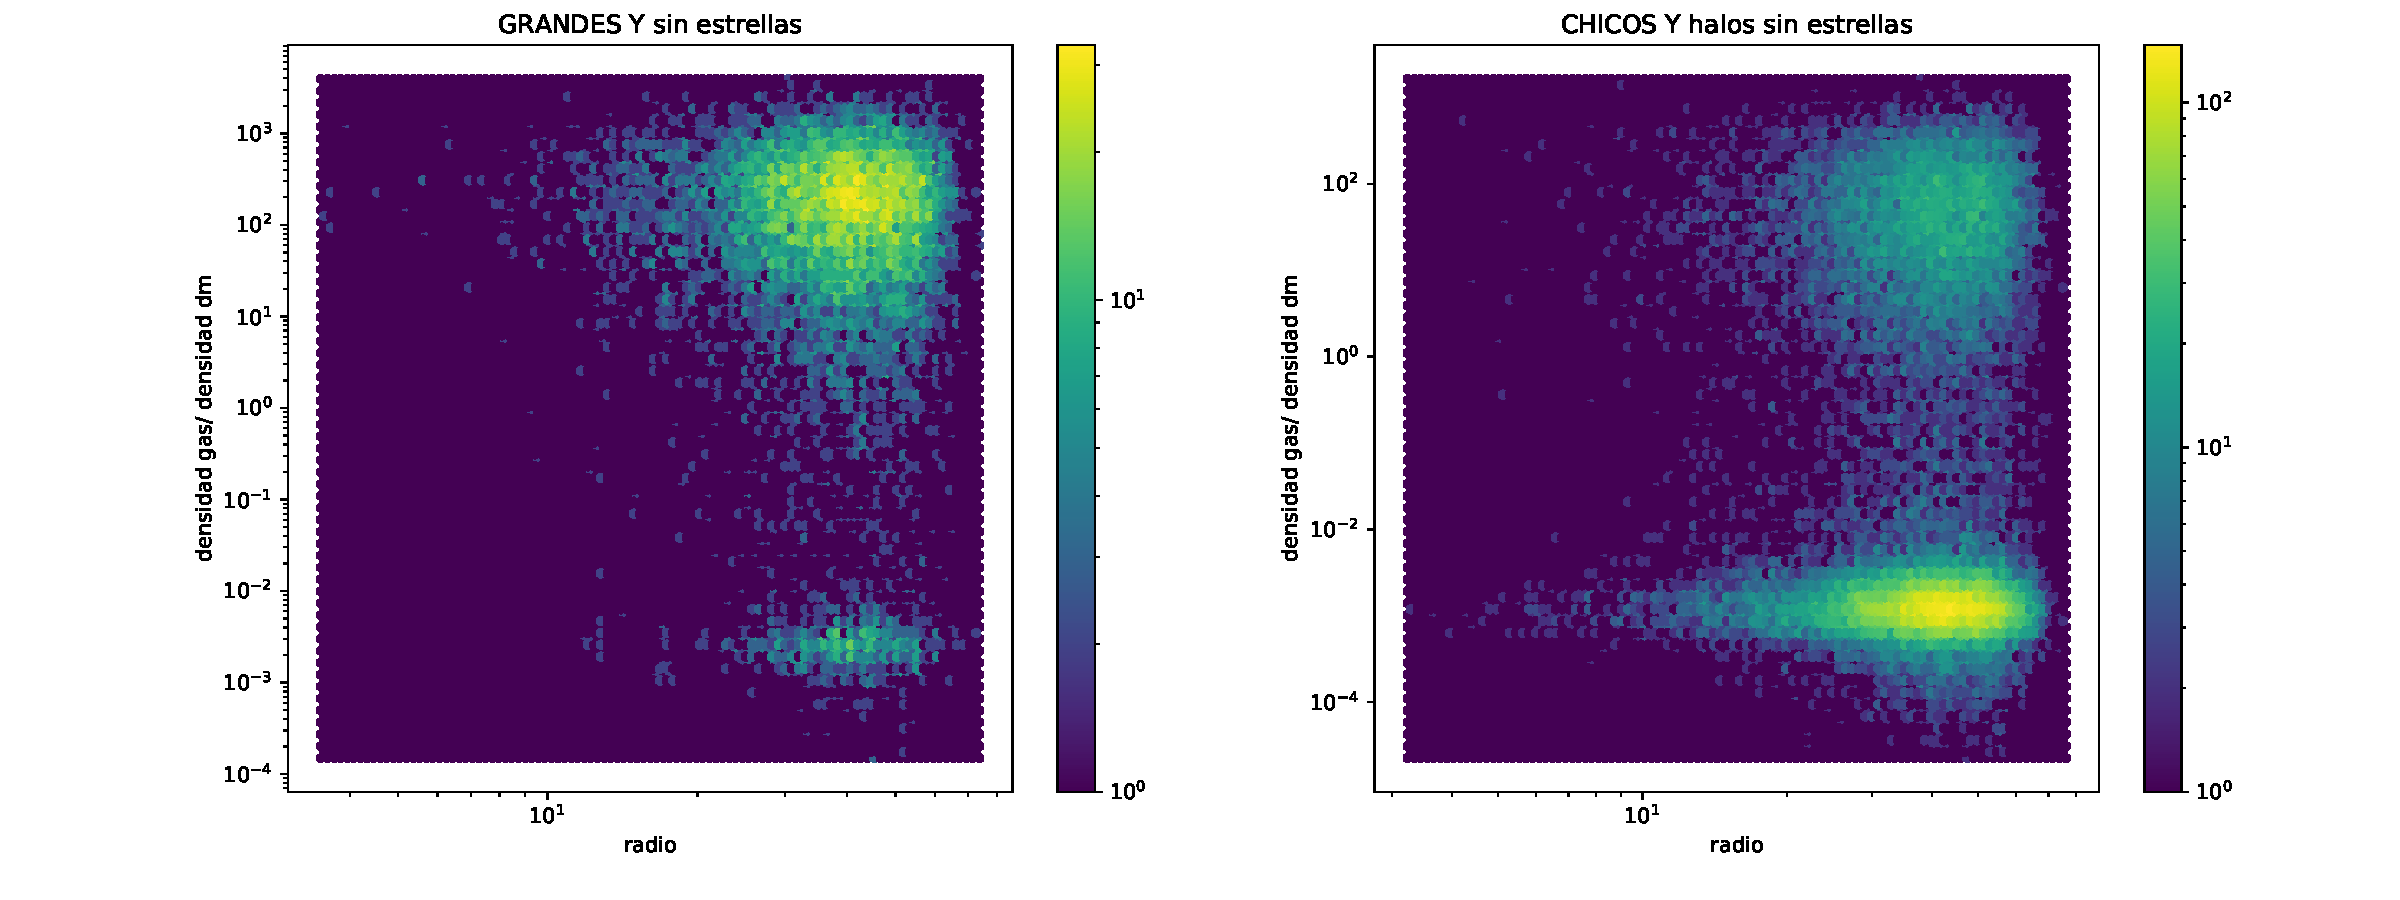
\includegraphics[width=18cm]{Figures/R_sctFRACC3.pdf}
\decoRule
\caption[perfil del void R]{}
\label{fig:Electron}
\end{figure}

\begin{figure}[h]
\centering
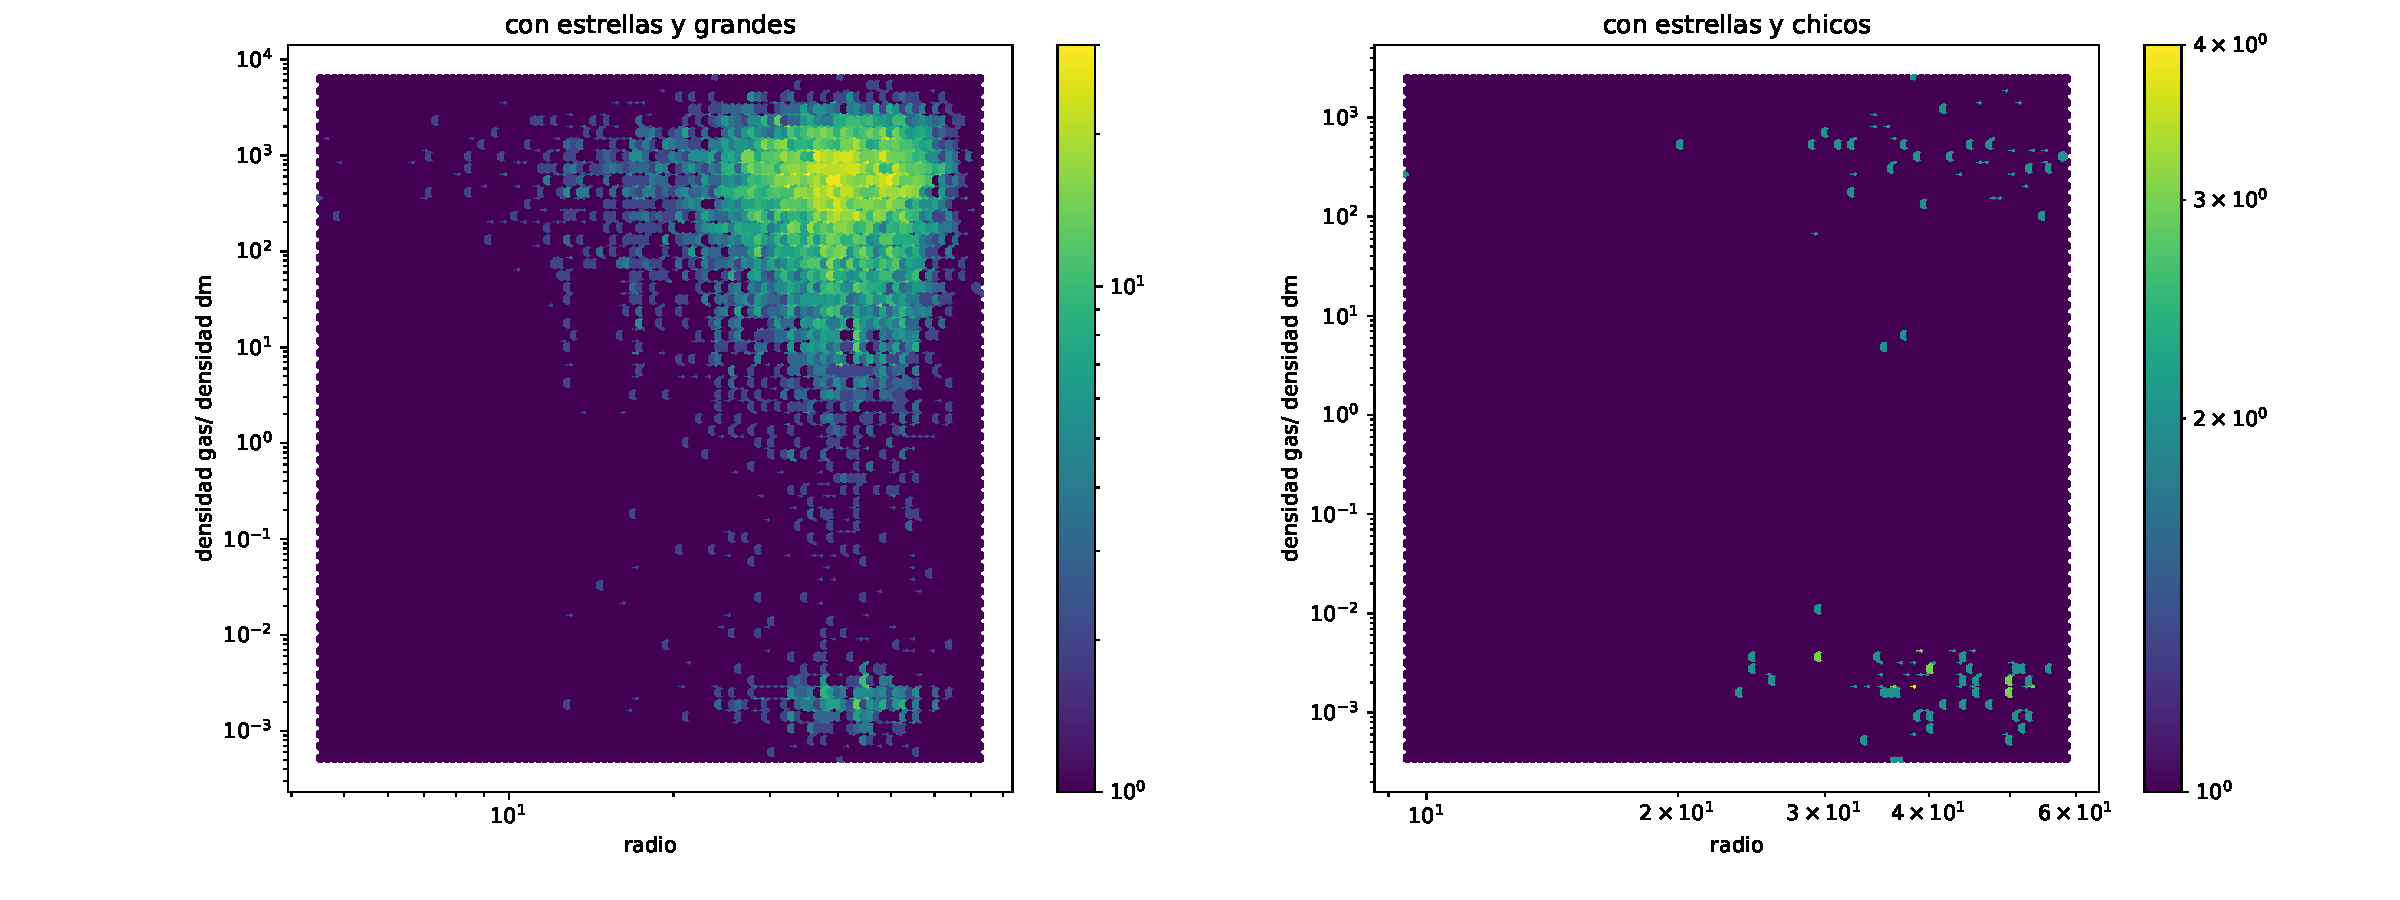
\includegraphics[width=18cm]{Figures/R_sctFRACC4.pdf}
\decoRule
\caption[perfil del void R]{}
\label{fig:Electron}
\end{figure}


\begin{figure}[h]
\centering
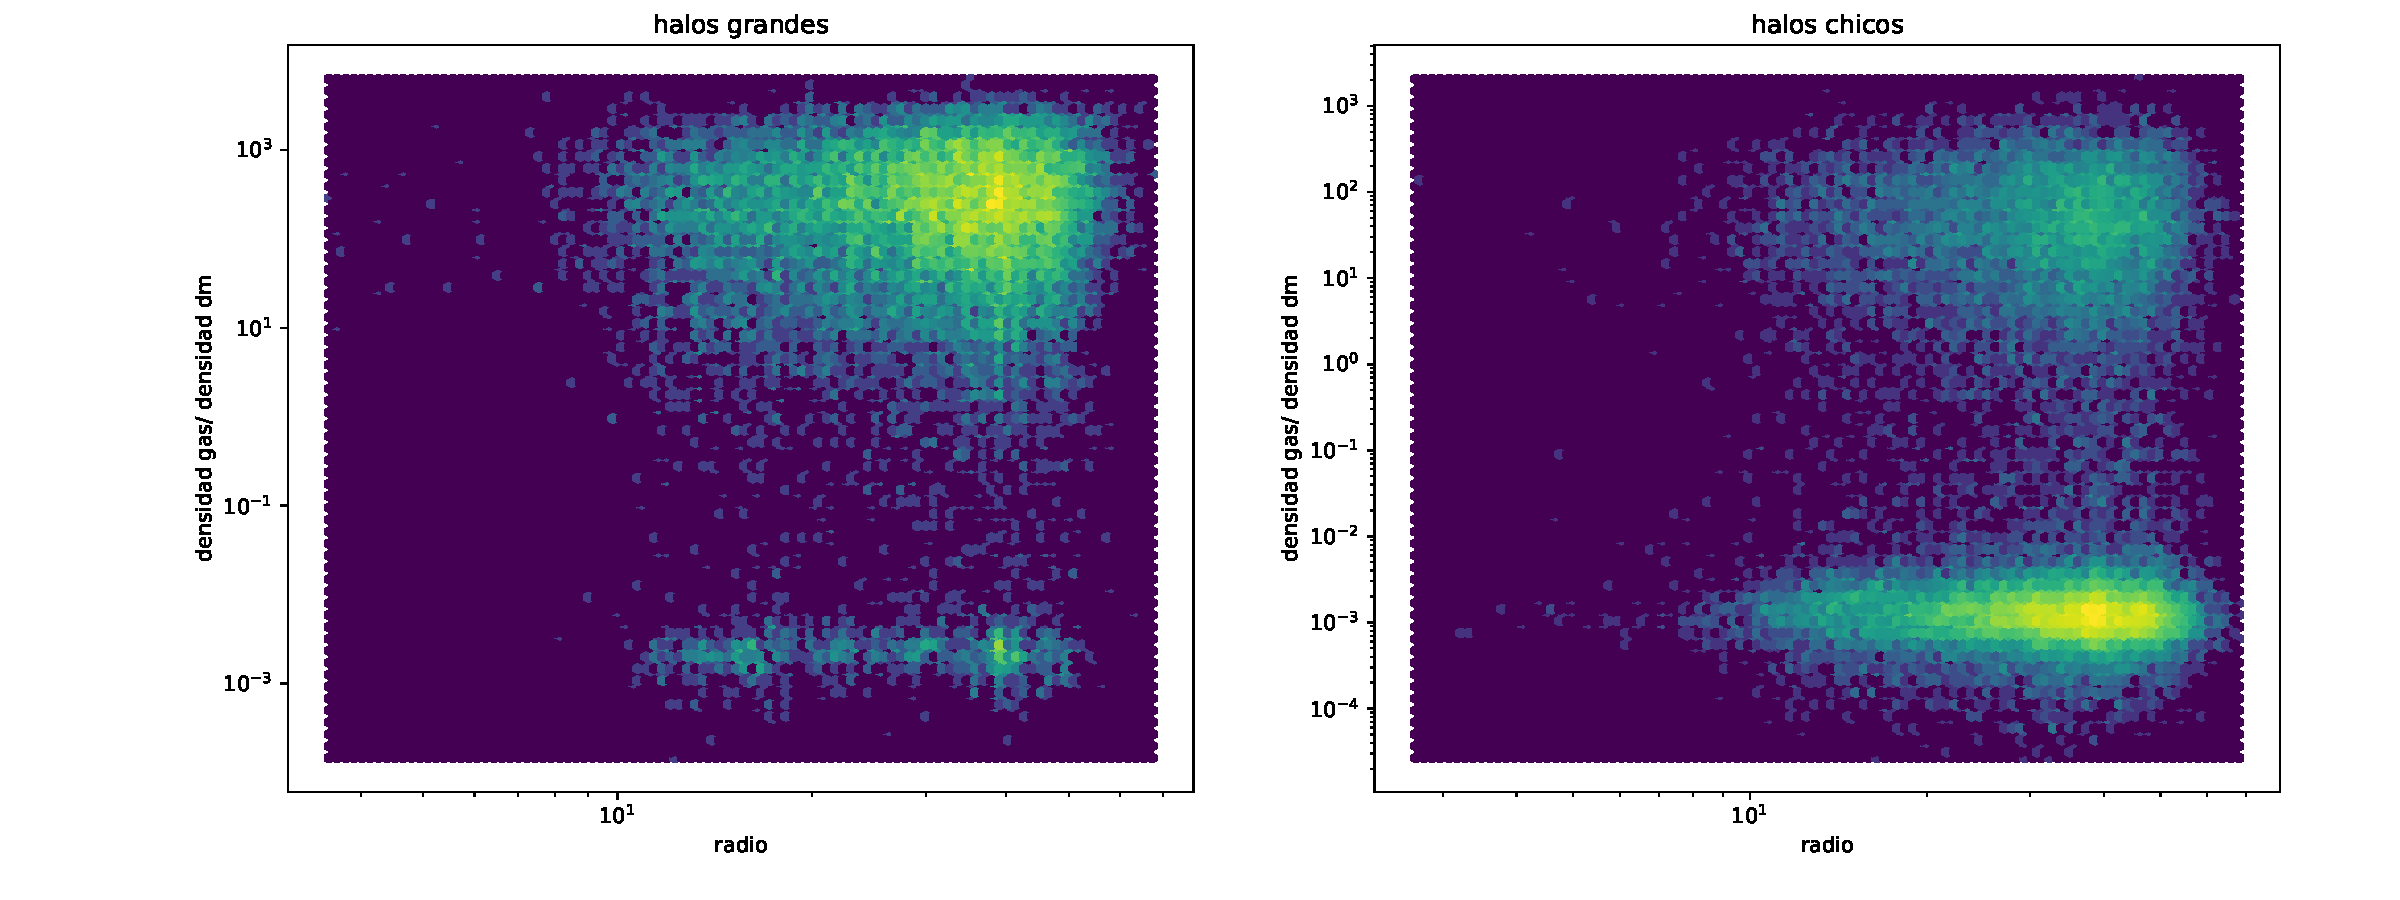
\includegraphics[width=18cm]{Figures/S_sctFRACC1.pdf}
\decoRule
\caption[perfil del void R]{}
\label{fig:Electron}
\end{figure}
\begin{figure}[h]
\centering
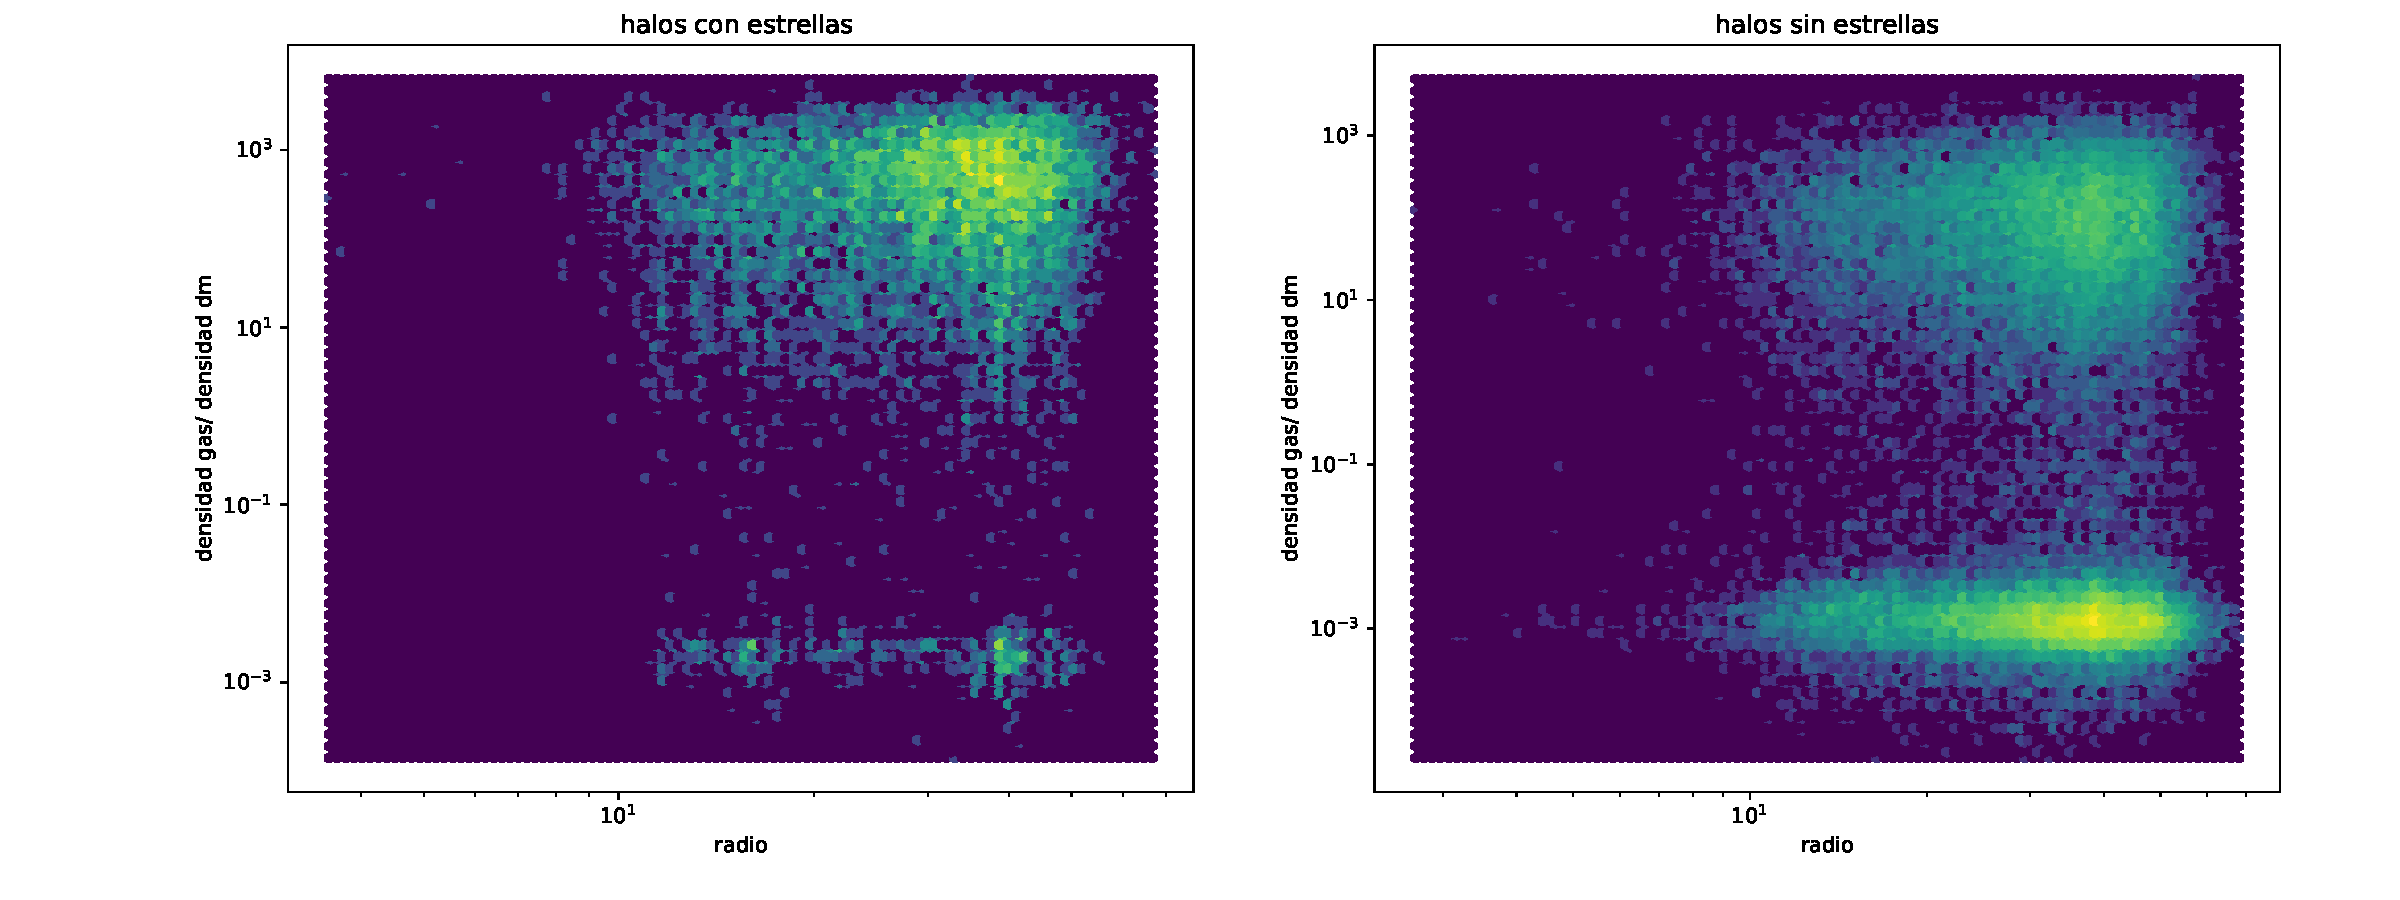
\includegraphics[width=18cm]{Figures/S_sctFRACC2.pdf}
\decoRule
\caption[perfil del void R]{}
\label{fig:Electron}
\end{figure}
\begin{figure}[h]
\centering
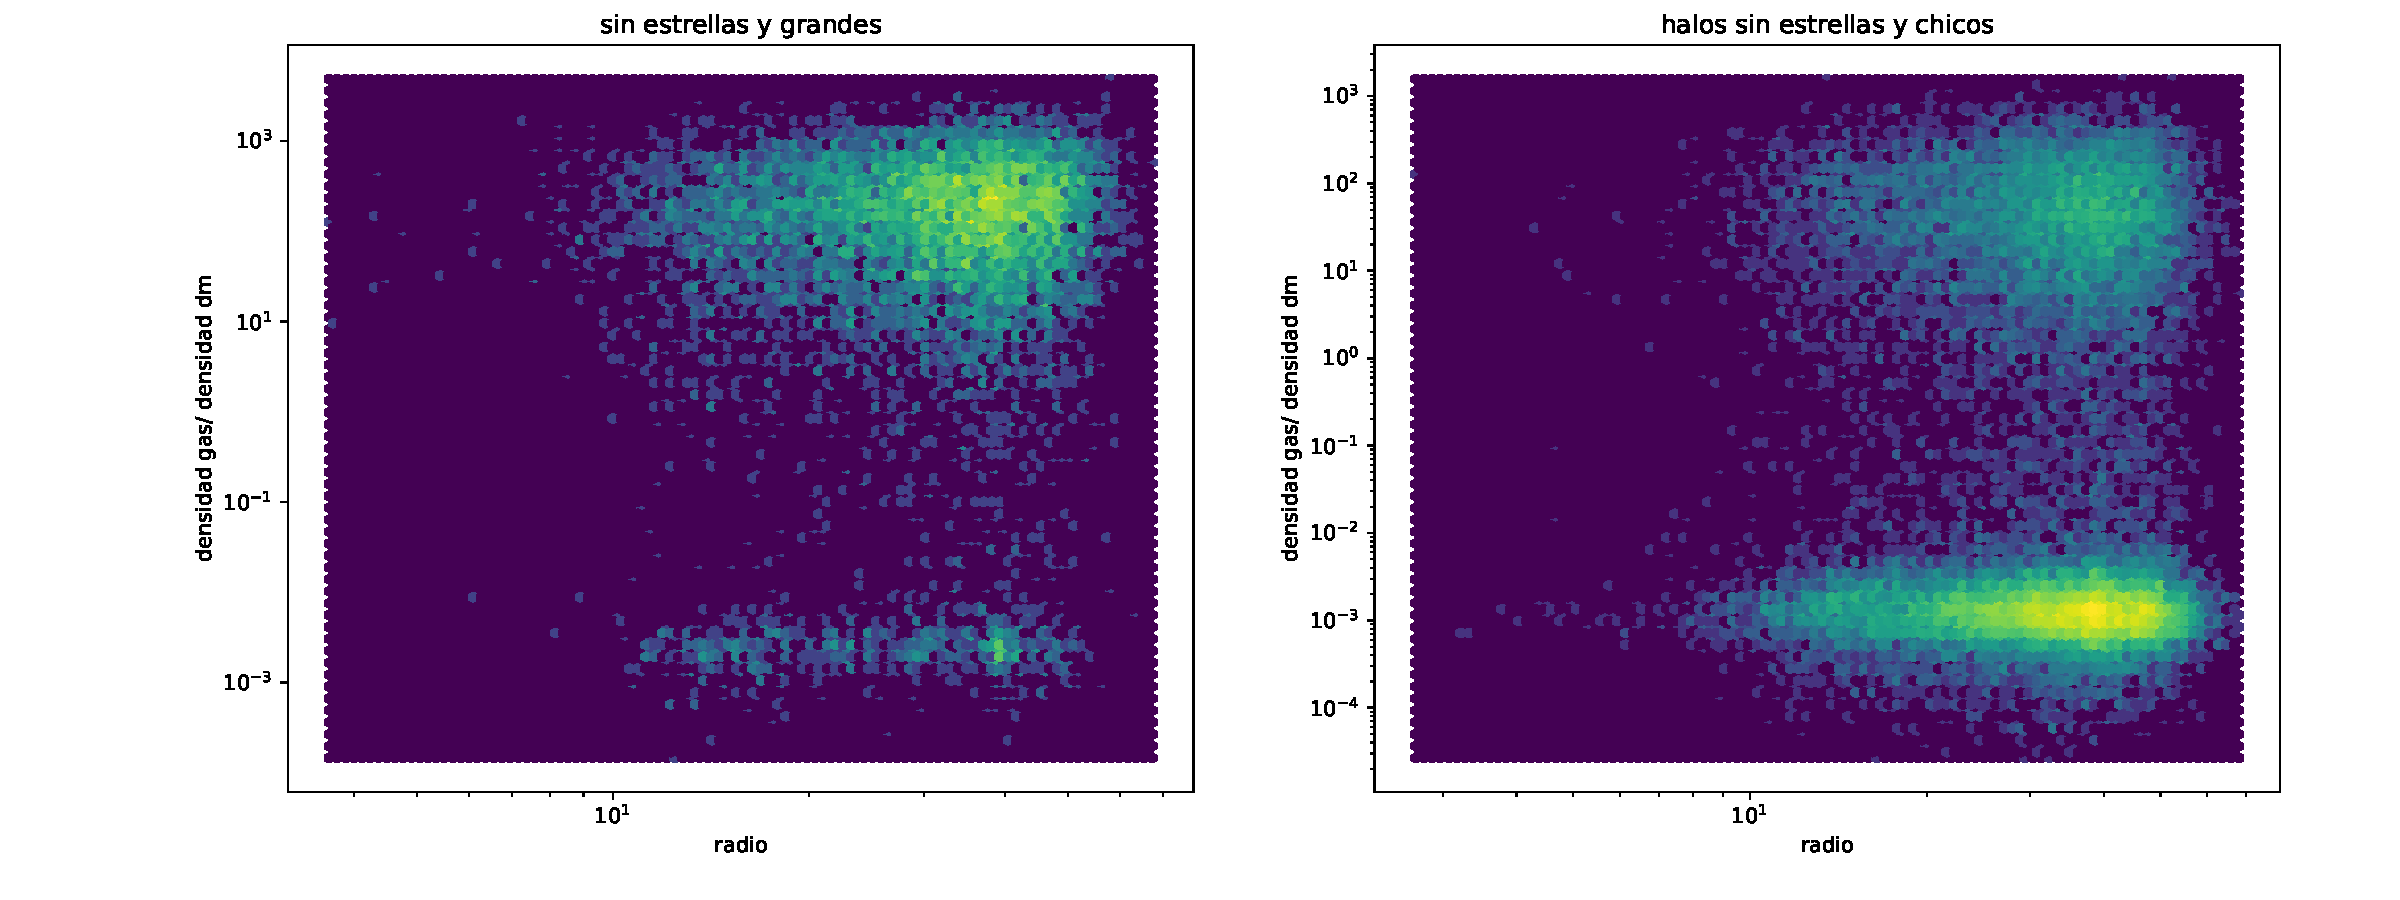
\includegraphics[width=18cm]{Figures/S_sctFRACC3.pdf}
\decoRule
\caption[perfil del void R]{}
\label{fig:Electron}
\end{figure}
\begin{figure}[h]
\centering
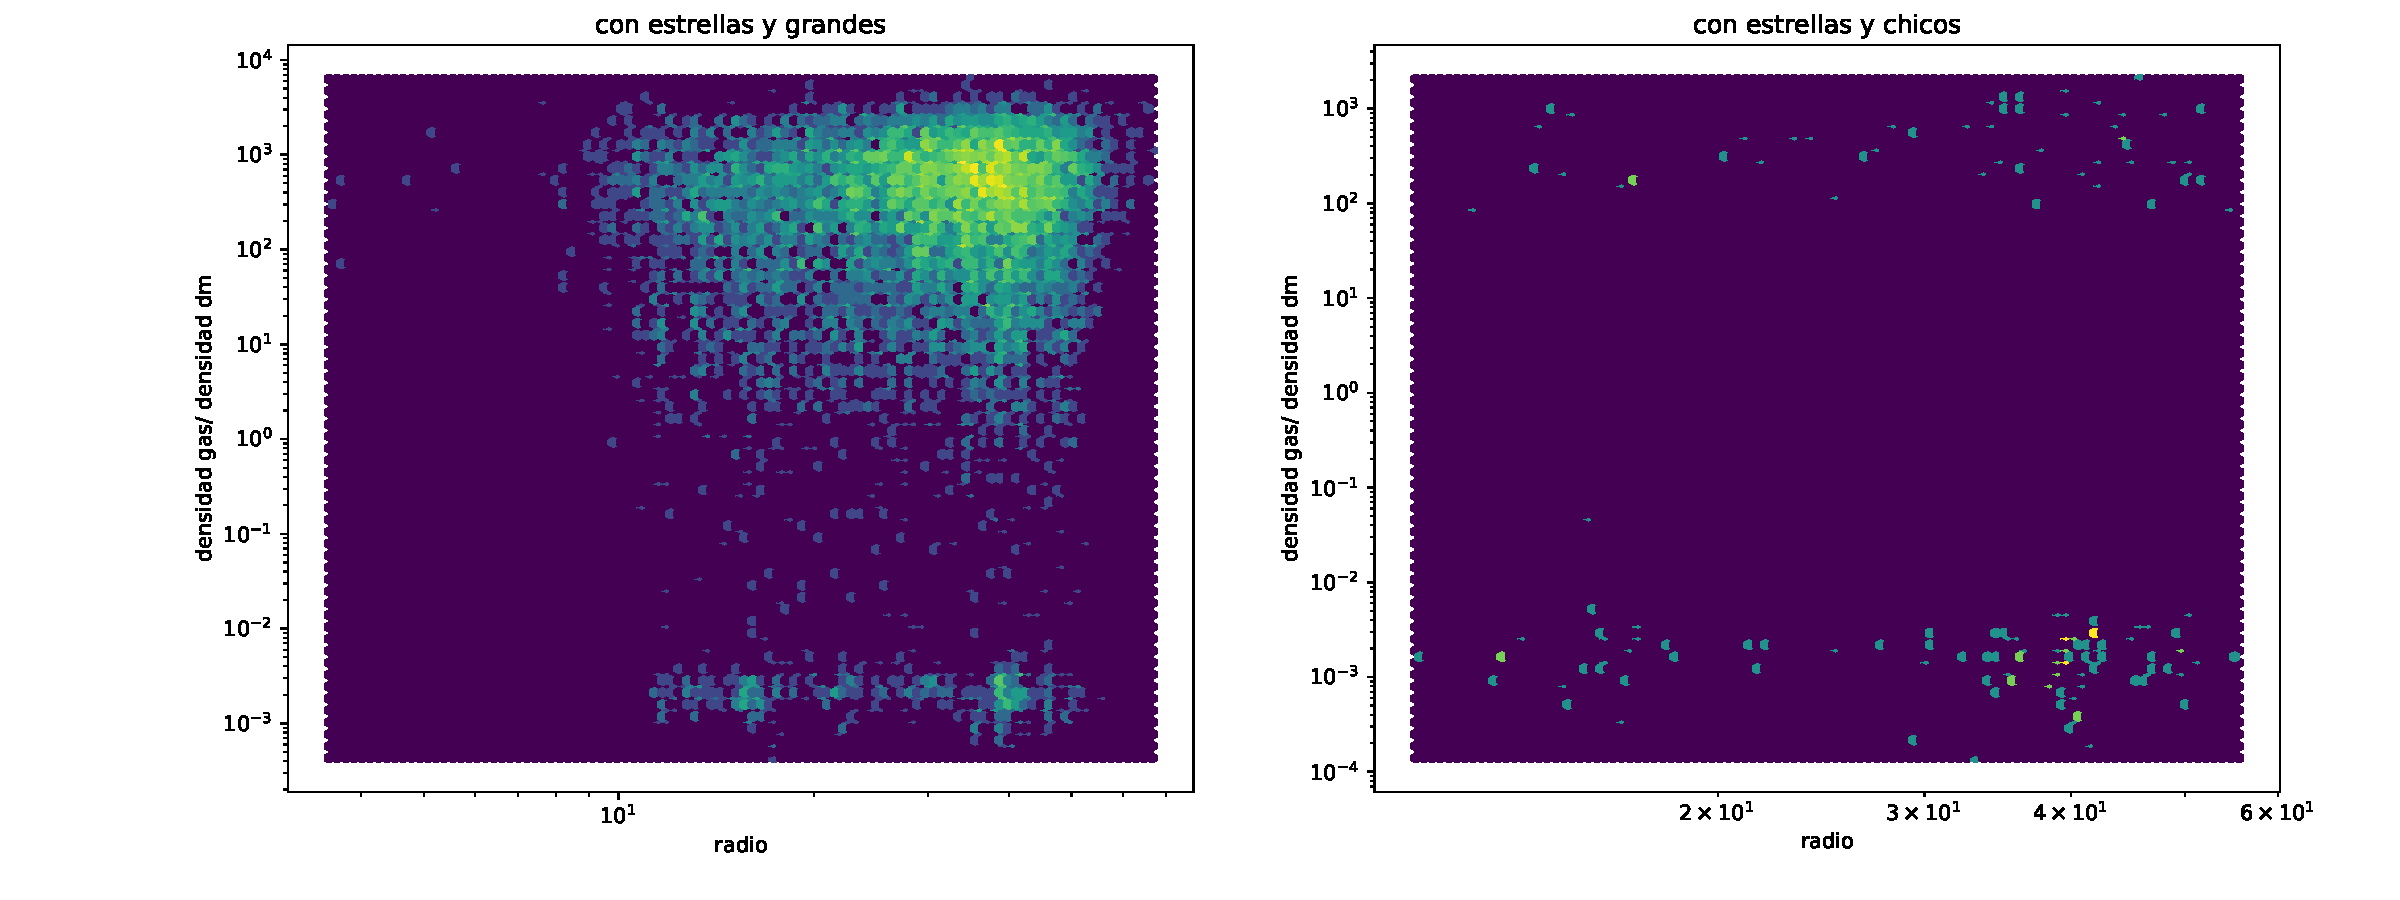
\includegraphics[width=18cm]{Figures/S_sctFRACC4.pdf}
\decoRule
\caption[perfil del void R]{}
\label{fig:Electron}
\end{figure}



\begin{figure}[h]
\centering
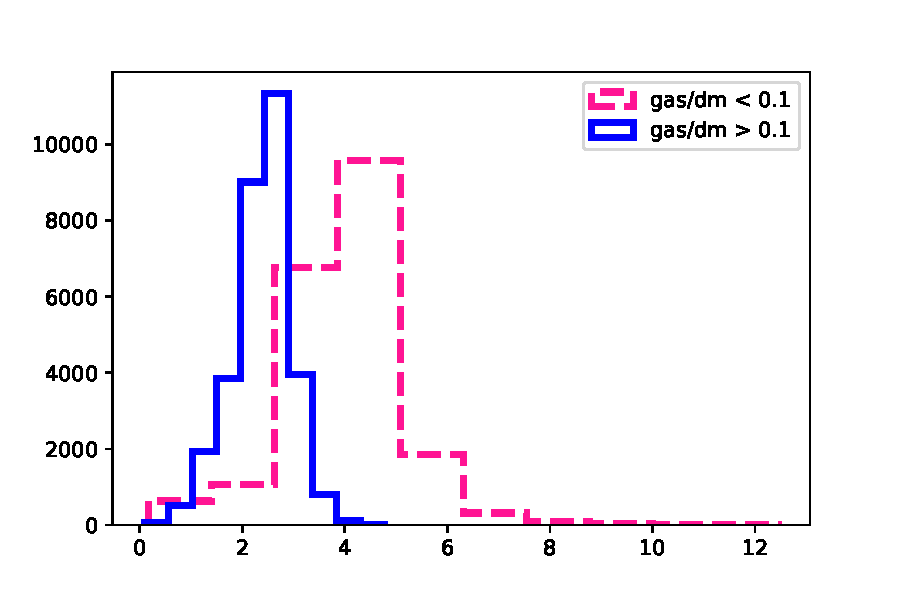
\includegraphics[width=10cm]{Figures/S_hsml.pdf}
\decoRule
\caption[asd]{VOID S distribucion para los maximo hsml/radio virial }
\label{fig:Electron}
\end{figure}

\begin{figure}[h]
\centering
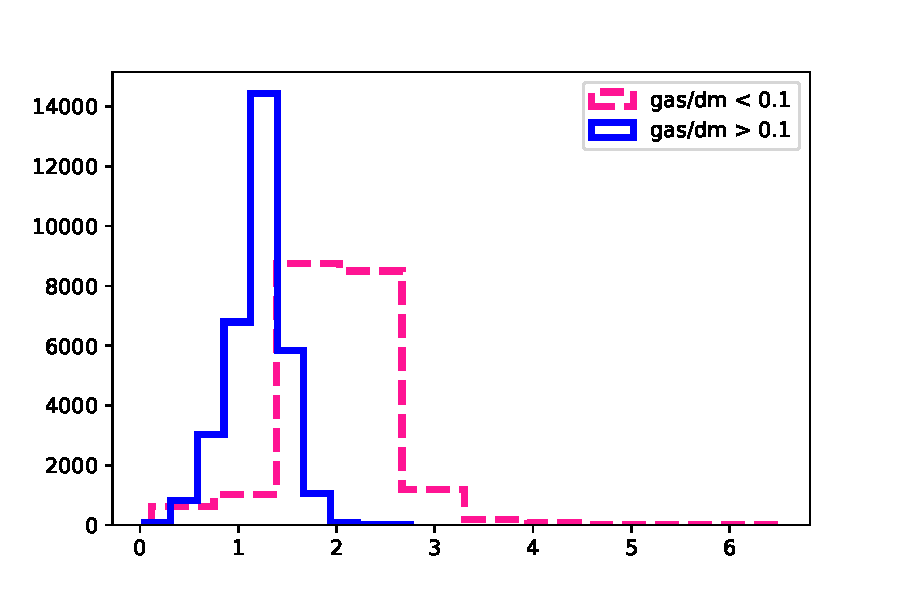
\includegraphics[width=10cm]{Figures/R_hsml.pdf}
\decoRule
\caption[asd]{VOID R distribucion para los maximo hsml/radio virial }
\label{fig:Electron}
\end{figure}

\begin{figure}[h]
\centering
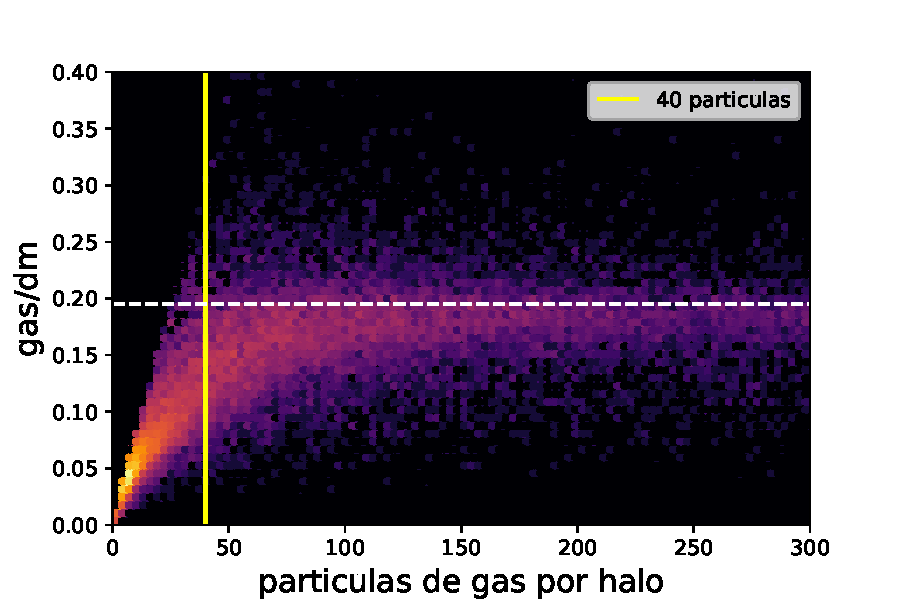
\includegraphics[width=18cm]{Figures/R_control1.pdf}
\decoRule
\caption[asd]{VOID R distribucion para los maximo hsml/radio virial }
\label{fig:Electron}
\end{figure}

\begin{figure}[h]
\centering
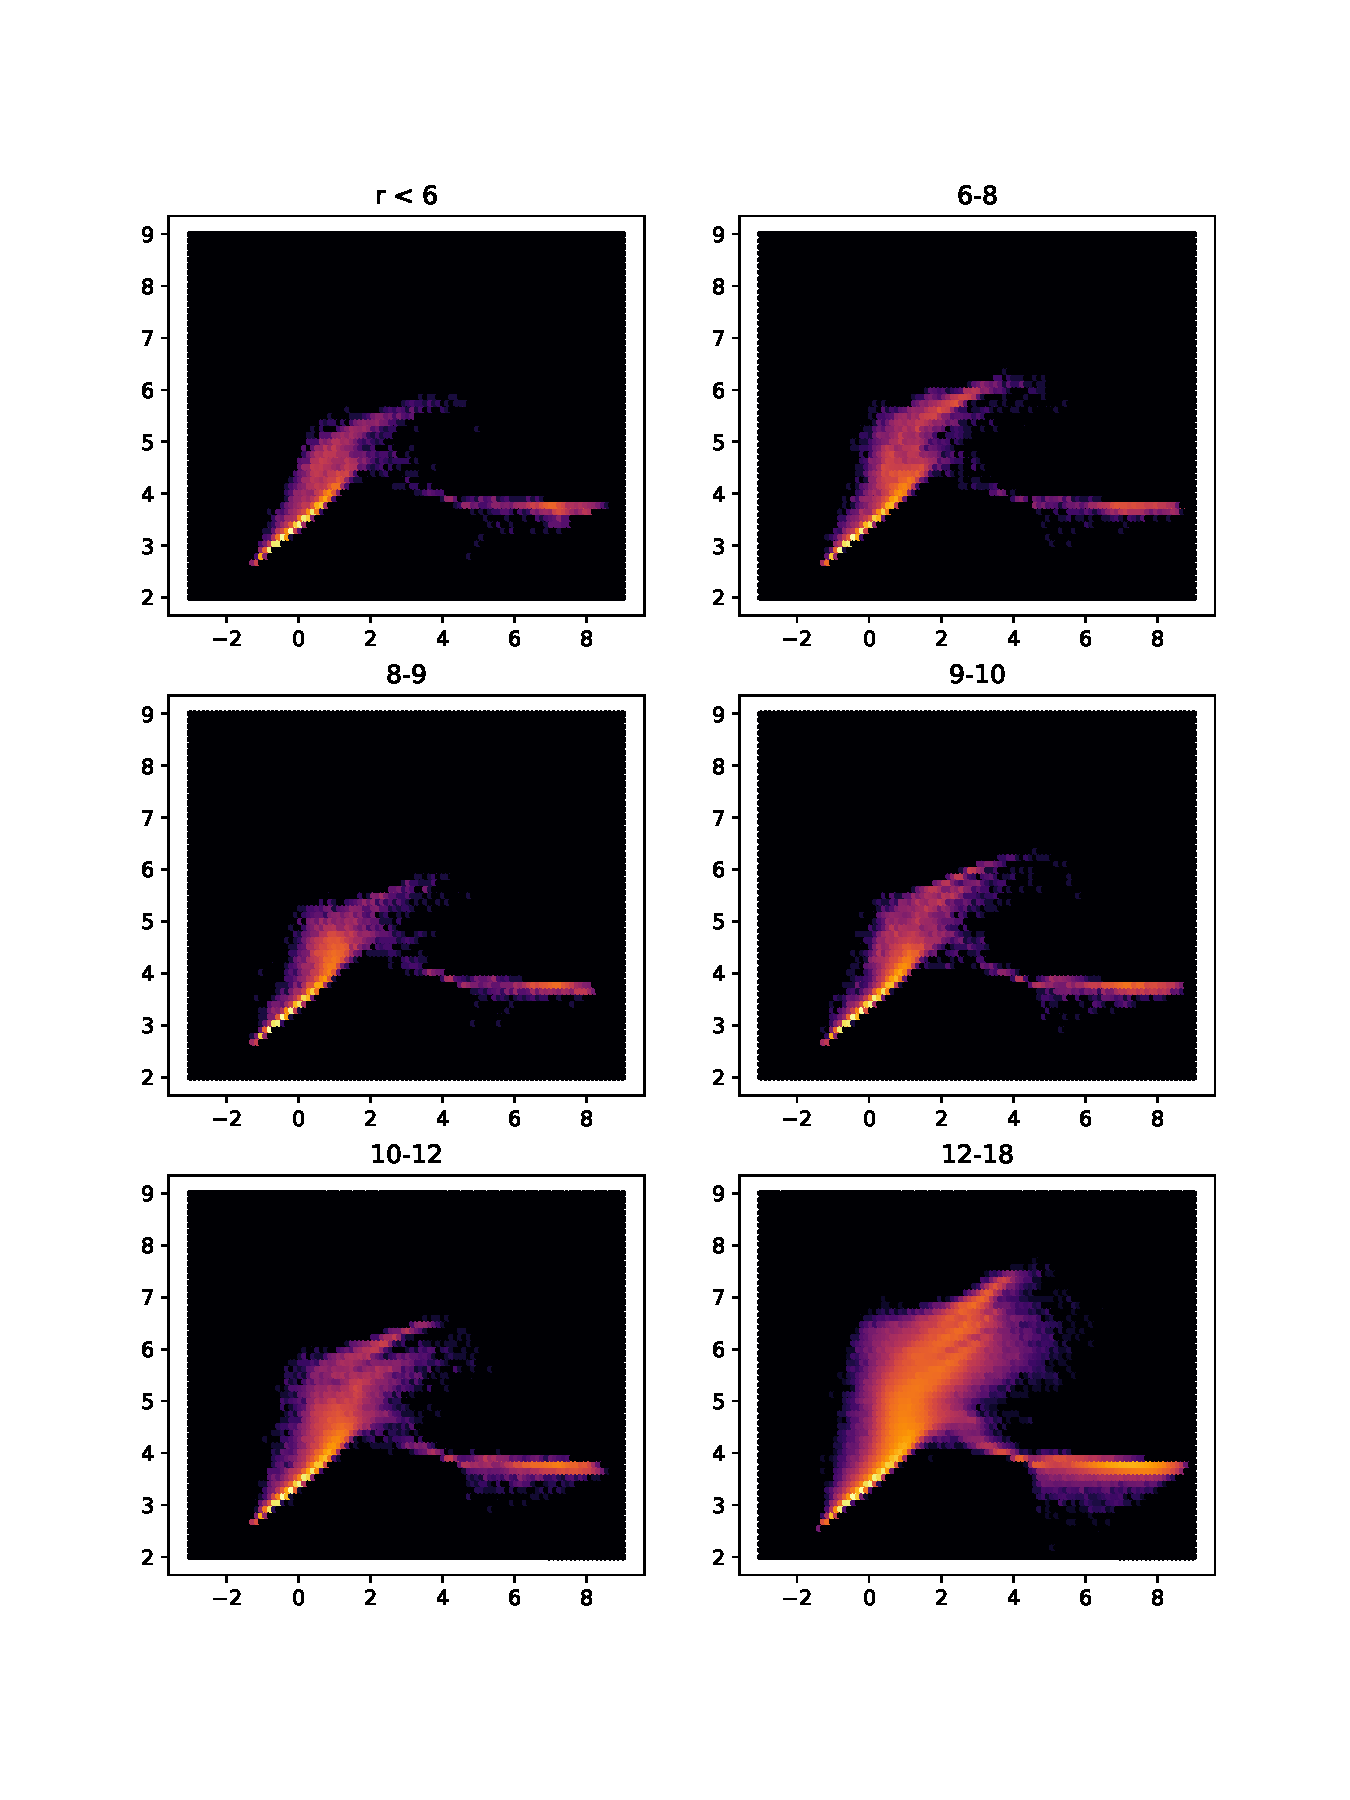
\includegraphics[width=15cm]{Figures/R1198_DF1.pdf}
\decoRule
\caption[asd]{diagramas de fase para el void R1198}
\label{fig:Electron}
\end{figure}

\begin{figure}[h]
\centering
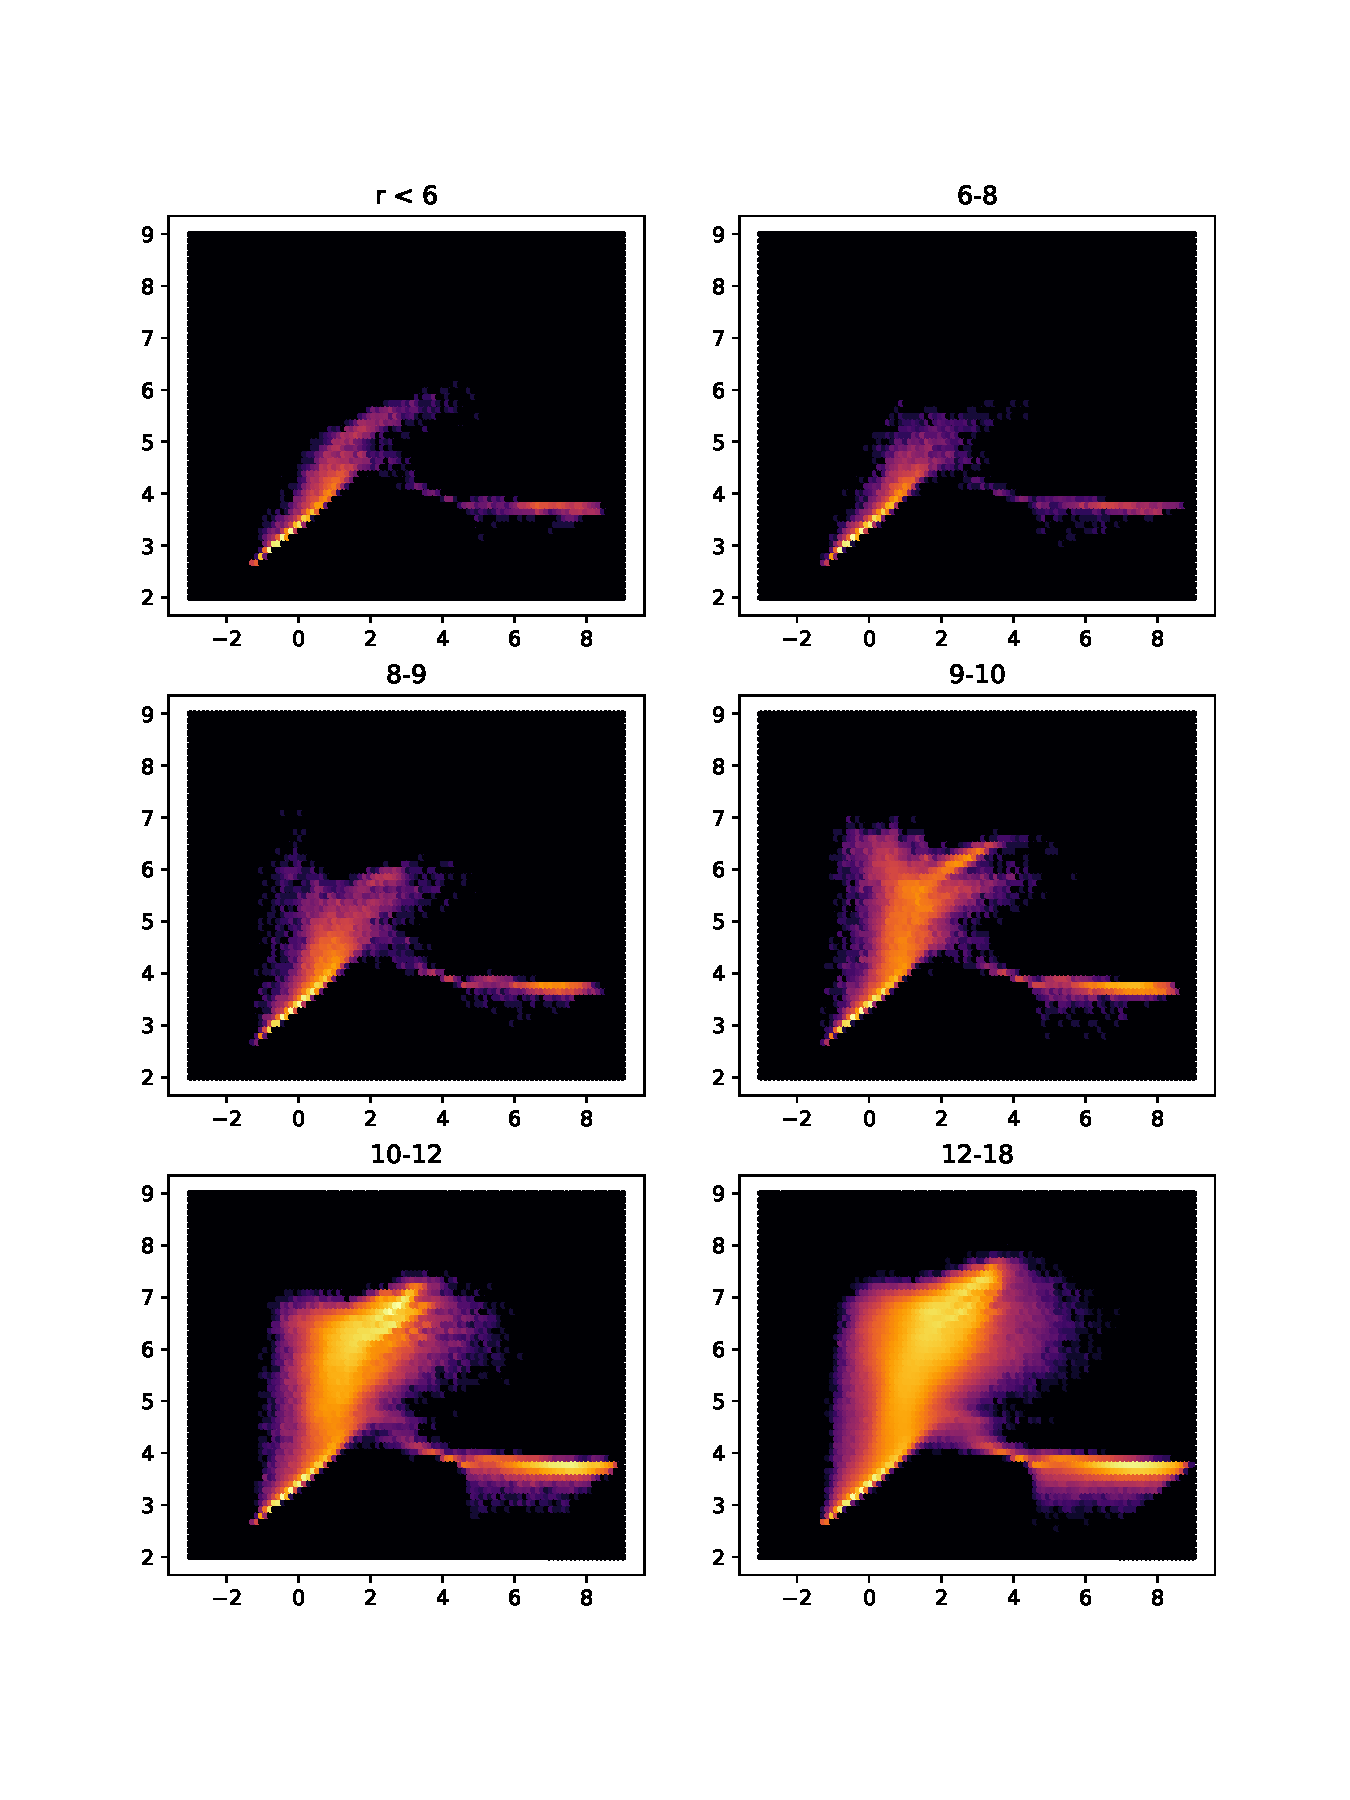
\includegraphics[width=15cm]{Figures/S1373_DF1.pdf}
\decoRule
\caption[asd]{diagramas de fase para el void S}
\label{fig:Electron}
\end{figure}

\begin{figure}[h]
\centering
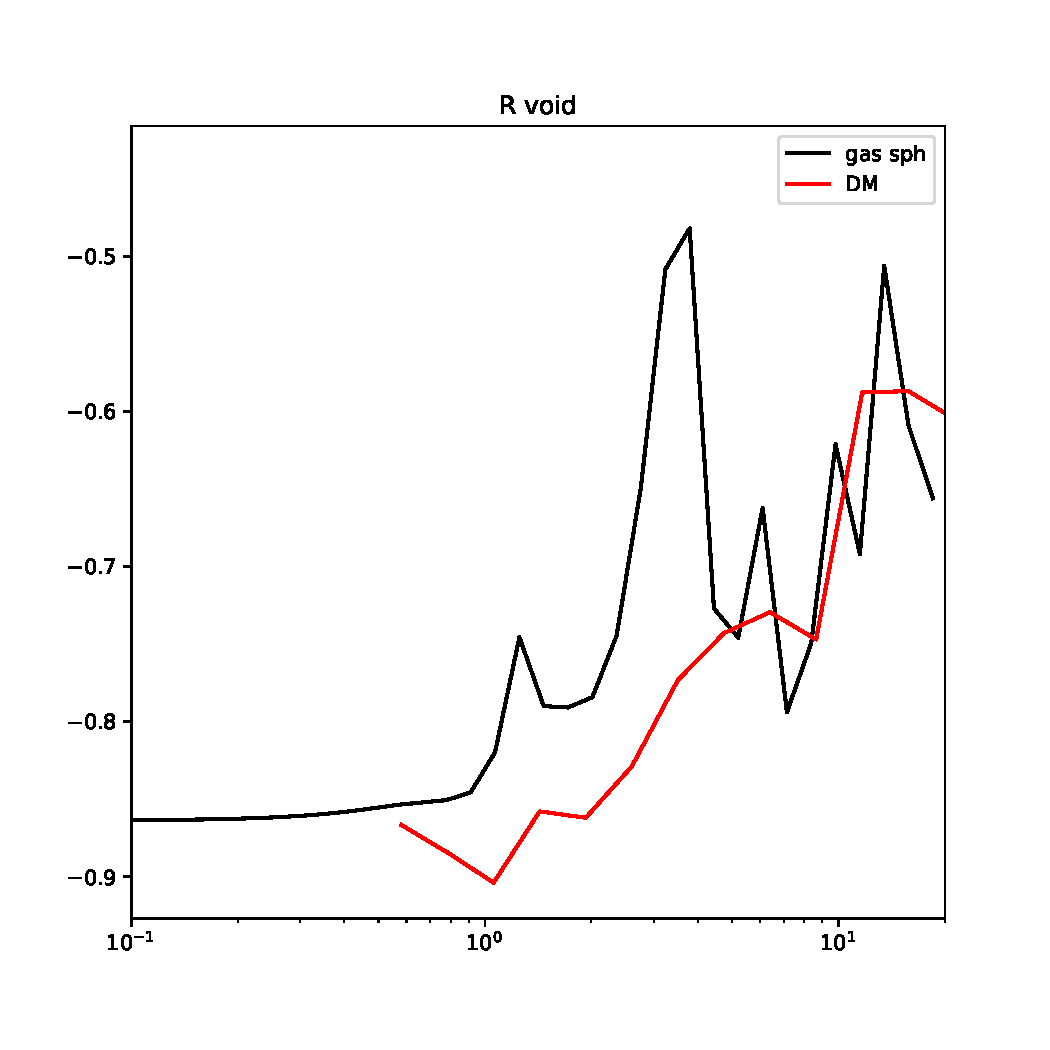
\includegraphics[width=15cm]{Figures/R1198_sph1.pdf}
\decoRule
\caption[asd]{diagramas de fase para el void S}
\label{fig:Electron}
\end{figure}

\begin{figure}[h]
\centering
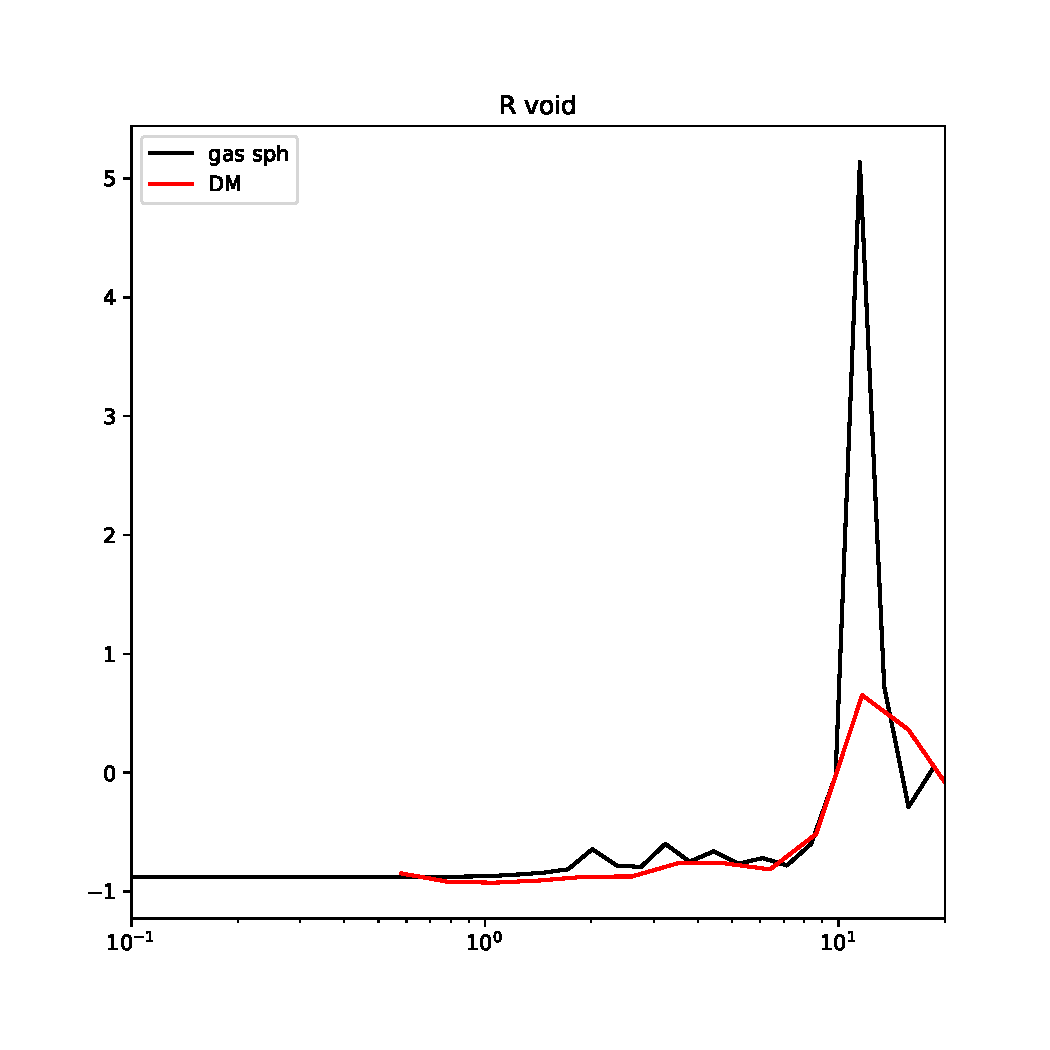
\includegraphics[width=15cm]{Figures/S1373_sph1.pdf}
\decoRule
\caption[asd]{diagramas de fase para el void S}
\label{fig:Electron}
\end{figure}

\begin{figure}[h]
\centering
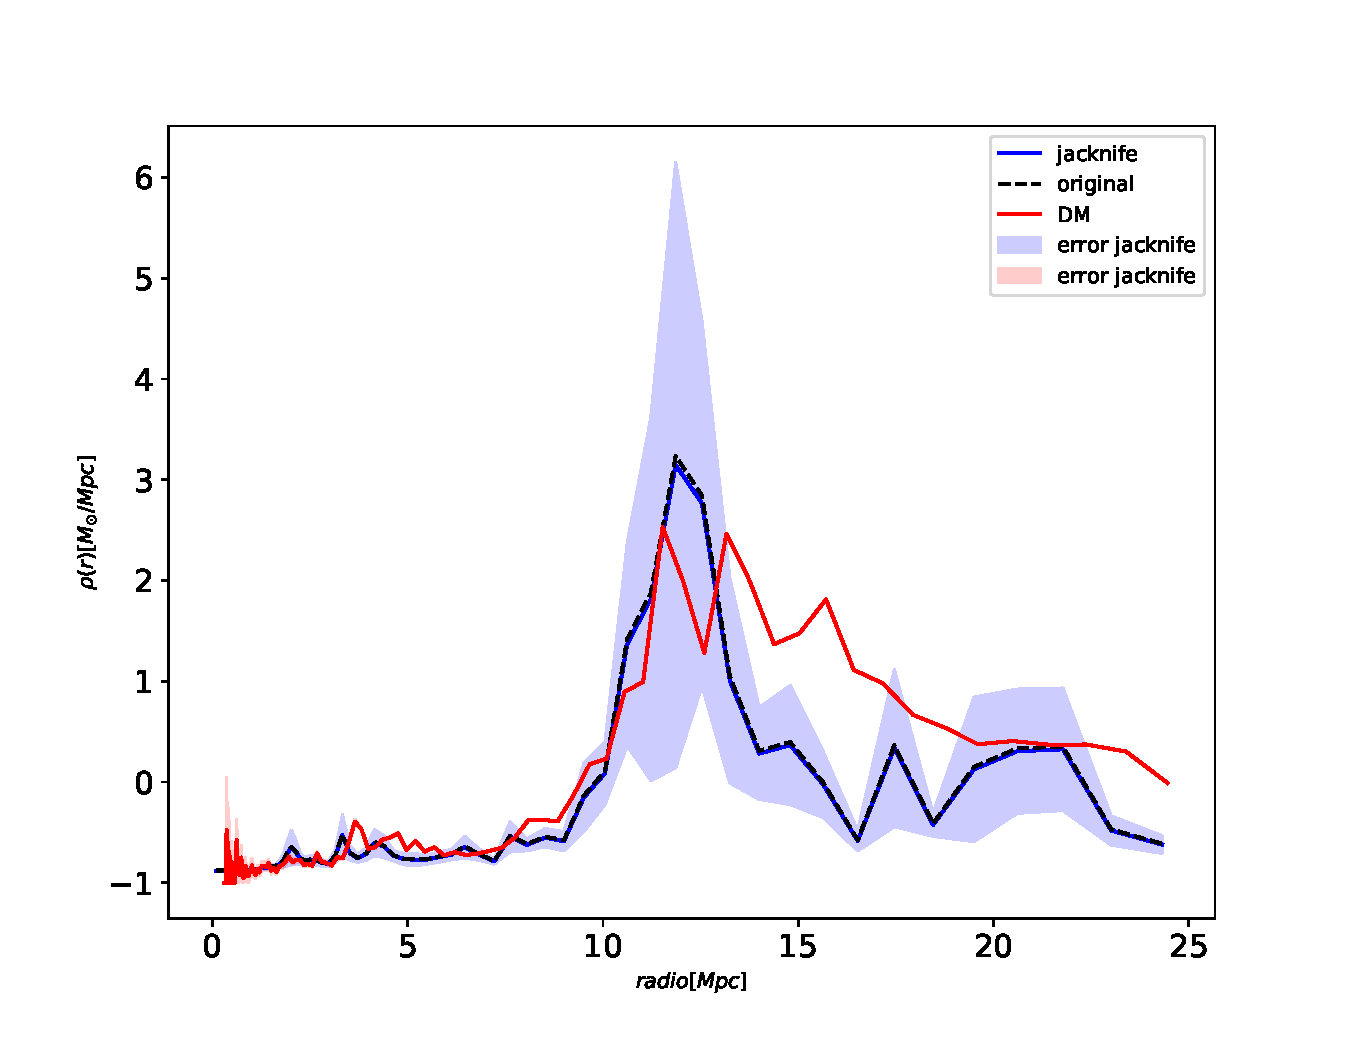
\includegraphics[width=15cm]{Figures/S1373_sph2.pdf}
\decoRule
\caption[asd]{diagramas de fase para el void S}
\label{fig:Electron}
\end{figure}

\begin{figure}[h]
\centering
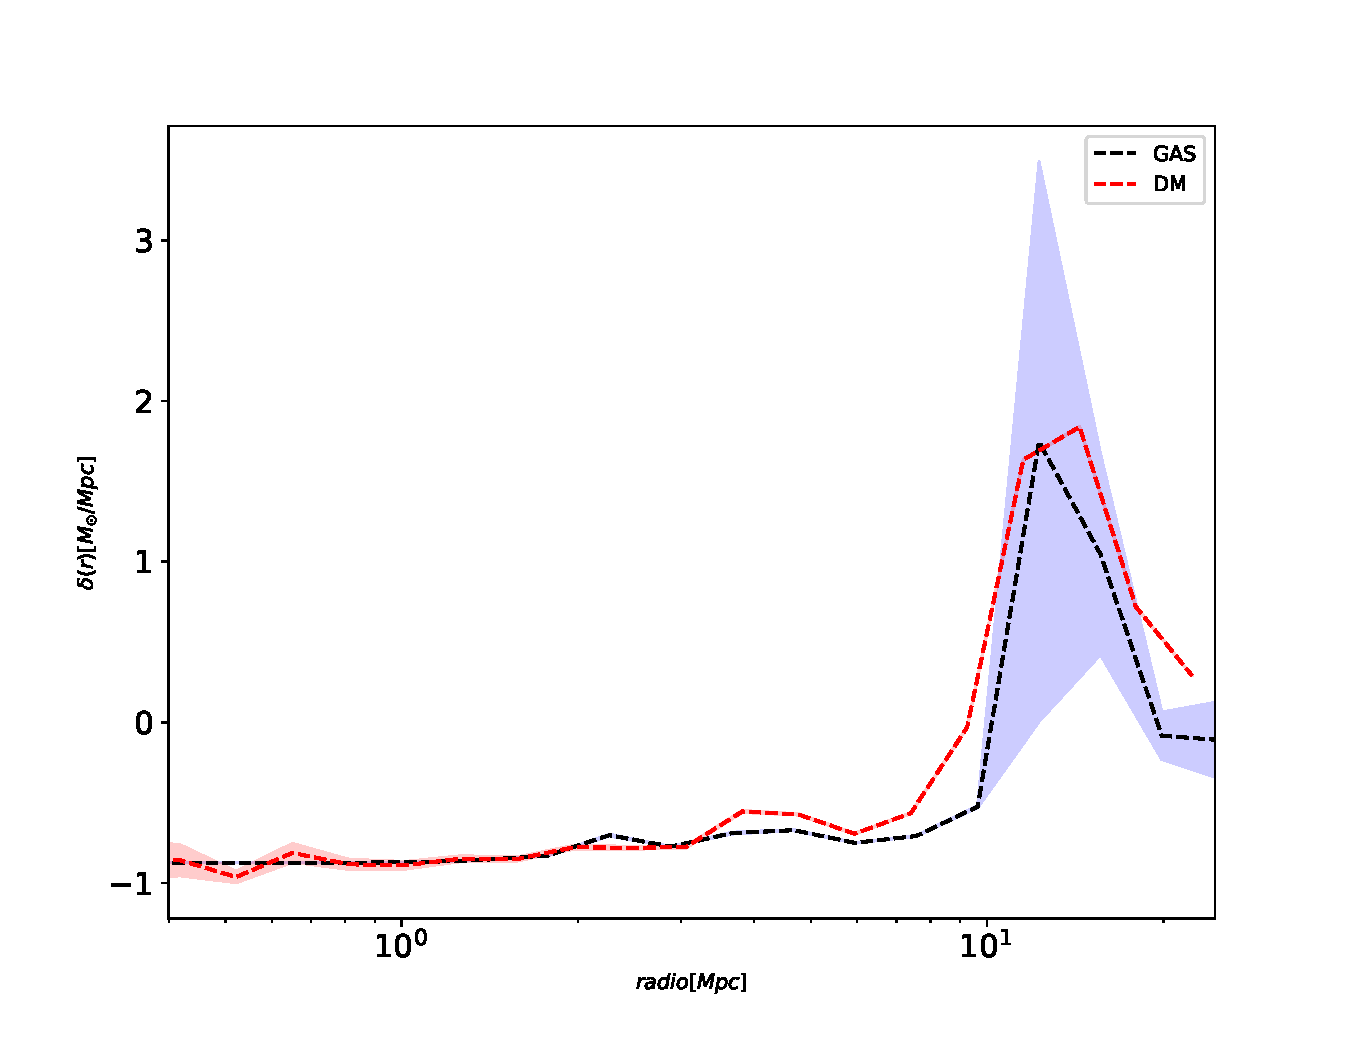
\includegraphics[width=15cm]{Figures/S1373_sph3.pdf}
\decoRule
\caption[asd]{Perfil de densidad diferencial para el void S. Se promediaron 200 muestras cada 10. }
\label{fig:Electron}
\end{figure}

\begin{figure}[h]
\centering
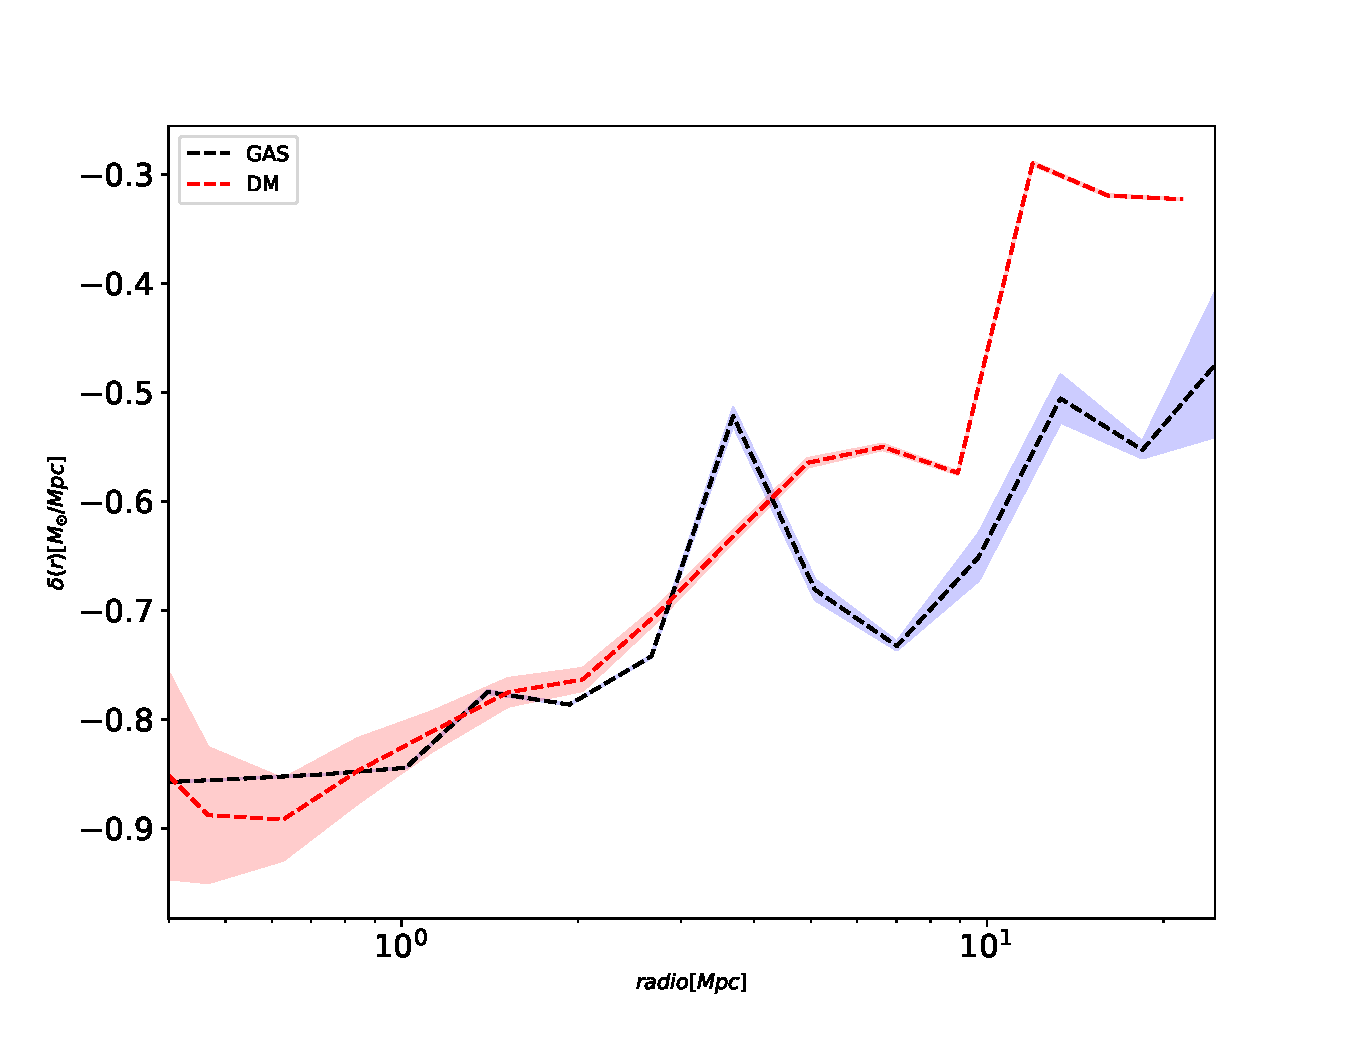
\includegraphics[width=15cm]{Figures/R1198_sph3.pdf}
\decoRule
\caption[asd]{Perfil de densidad diferencial para el void R. Se promediaron 200 muestras cada 10. }
\label{fig:Electron}
\end{figure}

\begin{figure}[h]
\centering
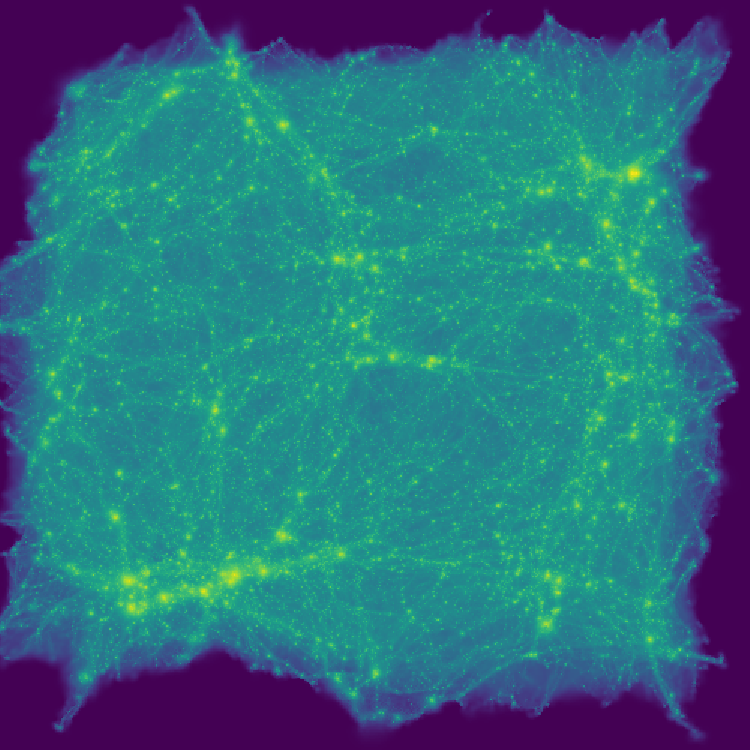
\includegraphics[width=15cm]{Figures/R1198_zoomin1.pdf}
\decoRule
\caption[asd]{resimulacion del void R }
\label{fig:Electron}
\end{figure}

\begin{figure}[h]
\centering
\includegraphics[width=15cm]{Figures/S1373_zoomin1.pdf}
\decoRule
\caption[asd]{resiumacion del void S }
\label{fig:Electron}
\end{figure} 

%----------------------------------------------------------------------------------------
%	THESIS CONTENT - APPENDICES
%----------------------------------------------------------------------------------------

\appendix % Cue to tell LaTeX that the following "chapters" are Appendices

% Include the appendices of the thesis as separate files from the Appendices folder
% Uncomment the lines as you write the Appendices

% Appendix A

\chapter{Frequently Asked Questions} % Main appendix title

\label{AppendixA} % For referencing this appendix elsewhere, use \ref{AppendixA}

\section{How do I change the colors of links?}

The color of links can be changed to your liking using:

{\small\verb!\hypersetup{urlcolor=red}!}, or

{\small\verb!\hypersetup{citecolor=green}!}, or

{\small\verb!\hypersetup{allcolor=blue}!}.

\noindent If you want to completely hide the links, you can use:

{\small\verb!\hypersetup{allcolors=.}!}, or even better: 

{\small\verb!\hypersetup{hidelinks}!}.

\noindent If you want to have obvious links in the PDF but not the printed text, use:

{\small\verb!\hypersetup{colorlinks=false}!}.

%\include{Appendices/AppendixB}
%\include{Appendices/AppendixC}

%----------------------------------------------------------------------------------------
%	BIBLIOGRAPHY
%----------------------------------------------------------------------------------------

\printbibliography[heading=bibintoc]

%----------------------------------------------------------------------------------------

\end{document}  
